% Saberes básicos (LOMLOE) asociados a esta unidad
%----------------------------------------------------------------------------------------
% A. Las destrezas científicas básicas
%   - Metodologías de la investigación científica: se introduce el método científico
%     (observación, hipótesis, experimentación, análisis de resultados y conclusiones) como
%     forma de trabajo propia de la física y la química, con ejemplos y un ejercicio de
%     identificación de sus fases en una investigación sencilla.
%   - El lenguaje científico: unidades del Sistema Internacional y sus símbolos: toda la unidad
%     gira en torno al SI (magnitud, unidad, medida), sus múltiplos y submúltiplos, y las reglas
%     de escritura correcta de los símbolos.
%   - Herramientas matemáticas básicas en diferentes escenarios científicos: uso de factores de
%     conversión, reglas de tres y ecuaciones sencillas (d = m/V) para resolver problemas
%     cuantitativos de conversión de unidades y de cálculo de magnitudes.
%   - Diversos entornos y recursos de aprendizaje científico como el laboratorio: manejo de
%     balanzas, probetas, buretas y pipetas; lectura correcta de instrumentos (menisco,
%     sensibilidad, precisión y exactitud de una medida).
%   - Normas de uso de cada espacio, asegurando y protegiendo así la salud propia y comunitaria
%     (identificación del material de laboratorio, normas generales de seguridad y pictogramas
%     de peligrosidad de los productos químicos, SGA/GHS) y el respeto hacia el medio ambiente.
%
% B. La materia
%   - Experimentos relacionados con los sistemas materiales: conocimiento y descripción de sus
%     propiedades (generales/características, cuantitativas/cualitativas, extensivas/intensivas),
%     su clasificación en cuerpos y sistemas materiales, y el uso de la densidad relativa para
%     predecir si un cuerpo flota o se hunde en un líquido.
%
% (Esta unidad no desarrolla contenidos de los bloques C -la energía-, D -la interacción- ni
% E -el cambio-, que se trabajan en unidades posteriores del curso.)
%
% (Traducción al español de Unit_1_Matter_Measurement.tex. Las secciones comentadas del
%  original —p. ej. «Science and the scientific method»— no se traducen.)
%----------------------------------------------------------------------------------------

\spacing{1.3}
\raggedbottom % pages with large figures end where the text ends (no stretched gaps between boxes)

%----------------------------------------------------------------------------------------

\section{La materia y sus propiedades}

\begin{definition}[Materia]
    Es todo lo que tiene \textbf{masa} y ocupa un \textbf{espacio}.
\end{definition}

\begin{figure}[H]
    \centering
    % [FIGURA ORIGINAL] \includegraphics[width=\textwidth]{Unit_1/matter_definition}
    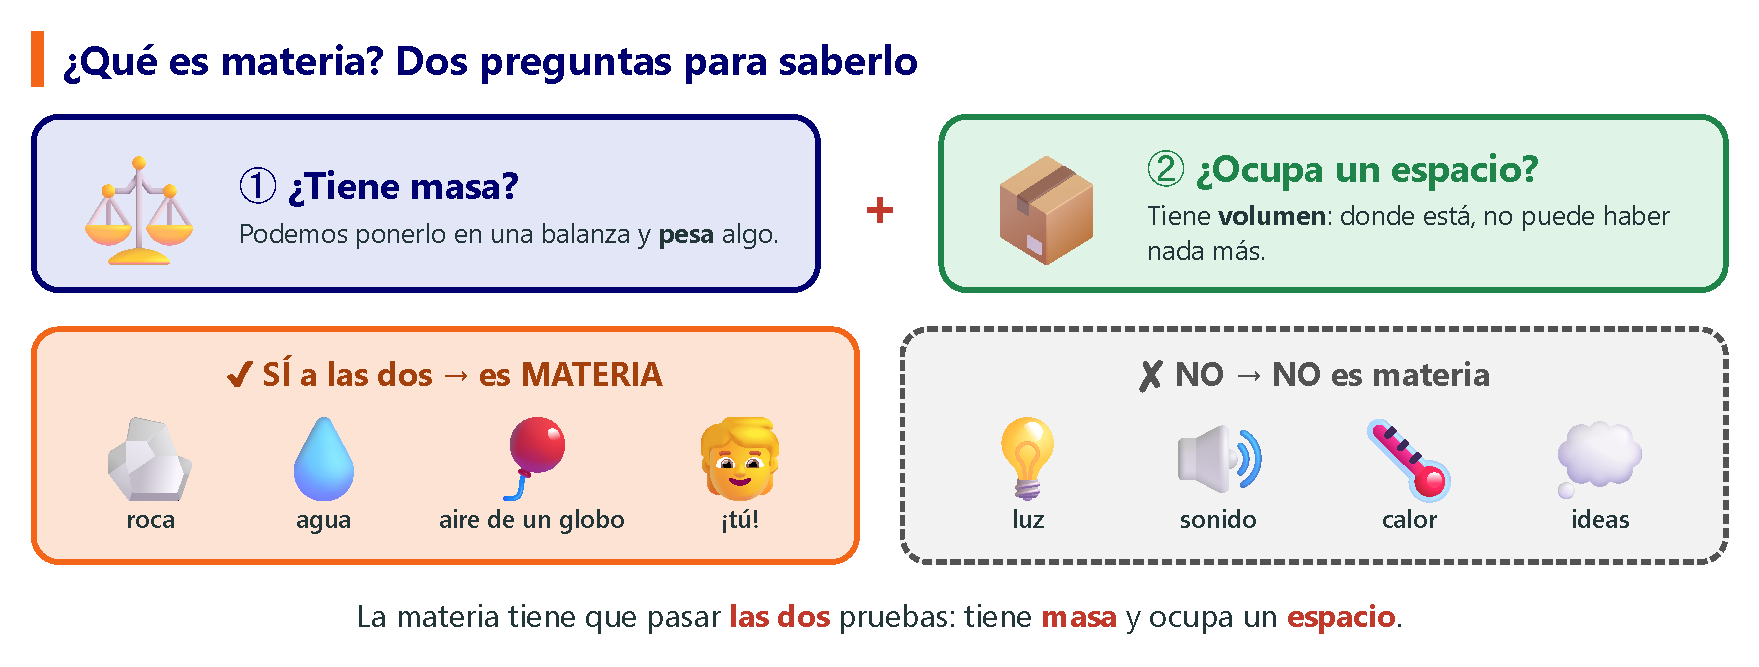
\includegraphics[width=\textwidth]{FigurasSVG/Unit_1_Matter_Measurement/pdf/matter_definition_es.pdf}
    \caption{Para ser materia, algo tiene que tener masa \textbf{y} ocupar un espacio. La luz, el sonido, el calor o las ideas no son materia.}
    \label{fig:u1_matter_definition}
\end{figure}

El banco en el que te sientas, el agua que bebes y tu propio cuerpo son materia. La materia se divide en dos grandes grupos: los \negsubro{cuerpos} y los \negsubro{sistemas materiales}.

\begin{definition}[Cuerpo]
    Es una porción de materia que tiene \textbf{forma propia} y \textbf{límites definidos}: vemos dónde empieza y dónde acaba. Por ejemplo, un balón, un lápiz, una silla o la Luna.
\end{definition}

\begin{definition}[Sistema material]
    Es una porción de materia que \textbf{no tiene forma propia} ni \textbf{límites definidos}: adopta la forma del recipiente que la contiene. Por ejemplo, la leche, el aire, el zumo o la gasolina.
\end{definition}

\begin{figure}[H]
    \centering
    % [FIGURA ORIGINAL] \includegraphics[width=\textwidth]{Unit_1/matter_scheme}
    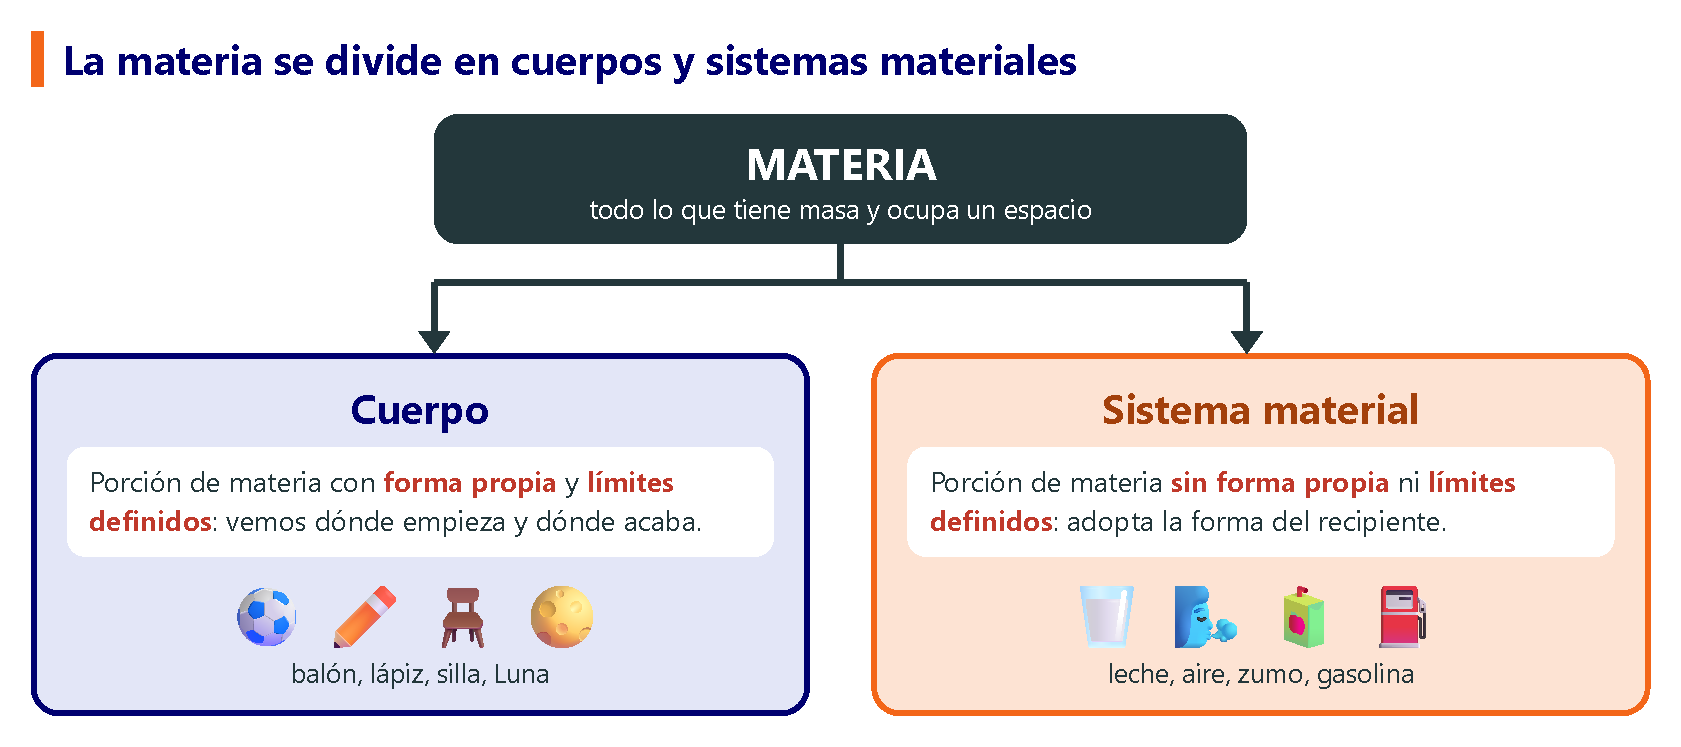
\includegraphics[width=\textwidth]{FigurasSVG/Unit_1_Matter_Measurement/pdf/matter_scheme_es.pdf}
    \caption{Esquema: la materia se divide en cuerpos y sistemas materiales.}
    \label{fig:u1_matter_scheme}
\end{figure}

\begin{figure}[H]
    \centering
    % [FIGURA ORIGINAL] \includegraphics[width=\textwidth]{Unit_1/matter_bodies}
    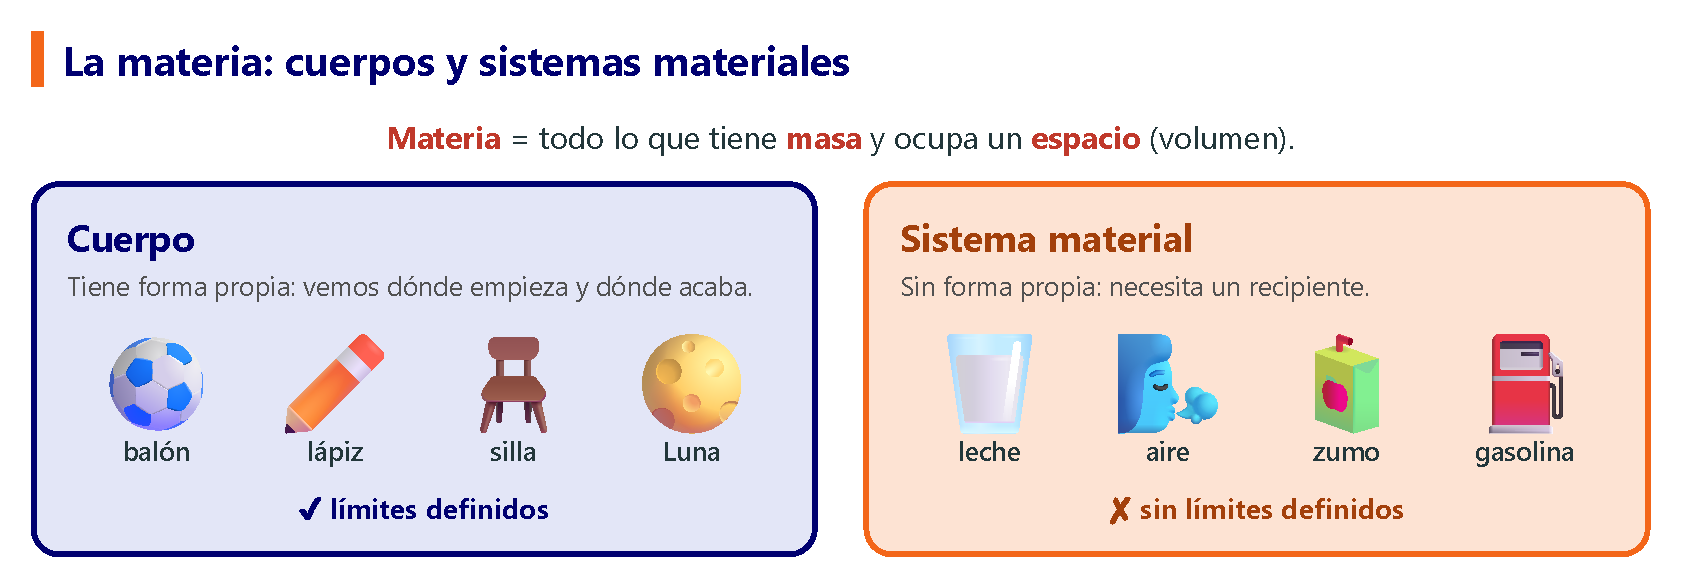
\includegraphics[width=\textwidth]{FigurasSVG/Unit_1_Matter_Measurement/pdf/matter_bodies_es.pdf}
    \caption{Los cuerpos tienen forma propia; los sistemas materiales necesitan un recipiente.}
    \label{fig:u1_matter_bodies}
\end{figure}

\begin{exercise}
    Indica si cada una de estas cosas es \textbf{materia} o \textbf{no es materia}. Recuerda: para ser materia debe tener masa \textbf{y} ocupar un lugar en el espacio.
    \begin{enumerate}[label=\letraminuscula]
        \item El aire de una habitación.
        \item La luz del Sol.
        \item Una piedra.
        \item El sonido de una campana.
        \item Una nube.
        \item El calor de un radiador.
        \item Un sueño.
        \item El humo de una hoguera.
        \item Un arcoíris.
        \item Una gota de aceite.
    \end{enumerate}
    \begin{solu}
        \begin{enumerate}[label=\alph*)]
            \item Materia (el aire tiene masa y llena la habitación).
            \item No es materia (la luz no tiene masa).
            \item Materia.
            \item No es materia (el sonido es una vibración que viaja a través de la materia, pero no es materia).
            \item Materia (está formada por gotitas de agua).
            \item No es materia (el calor es energía).
            \item No es materia (una idea no tiene masa ni ocupa espacio).
            \item Materia (está formado por gases y pequeñas partículas sólidas).
            \item No es materia (es luz).
            \item Materia.
        \end{enumerate}
    \end{solu}
\end{exercise}

\begin{exercise}
    Indica si cada una de estas porciones de materia es un \textbf{cuerpo} o un \textbf{sistema material}:
    \begin{enumerate}[label=\letraminuscula]
        \item Una moneda.
        \item El agua del mar.
        \item Una llave.
        \item El oxígeno de dentro de un globo.
        \item La miel.
        \item Un lápiz.
        \item El aceite de oliva.
        \item Una canica de cristal.
        \item El vapor de agua.
        \item Una pelota de tenis.
    \end{enumerate}
    \begin{solu}
        \begin{enumerate}[label=\alph*)]
            \item Cuerpo (forma propia y límites definidos).
            \item Sistema material (toma la forma del fondo del mar o del recipiente).
            \item Cuerpo.
            \item Sistema material (el gas toma la forma del globo).
            \item Sistema material (toma la forma del tarro).
            \item Cuerpo.
            \item Sistema material.
            \item Cuerpo.
            \item Sistema material.
            \item Cuerpo.
        \end{enumerate}
    \end{solu}
\end{exercise}

\subsection{La física y la química}

La física y la química son las dos ciencias que estudian la materia y sus cambios:

\begin{itemize}
    \item La \textbf{física} estudia los \negsubro{cambios físicos}: la sustancia sigue siendo \textbf{la misma}.
    \item La \textbf{química} estudia los \negsubro{cambios químicos}: aparecen \textbf{sustancias nuevas}.
\end{itemize}

\begin{figure}[H]
    \centering
    % [FIGURA ORIGINAL] \includegraphics[width=\textwidth]{Unit_1/physical_chemical}
    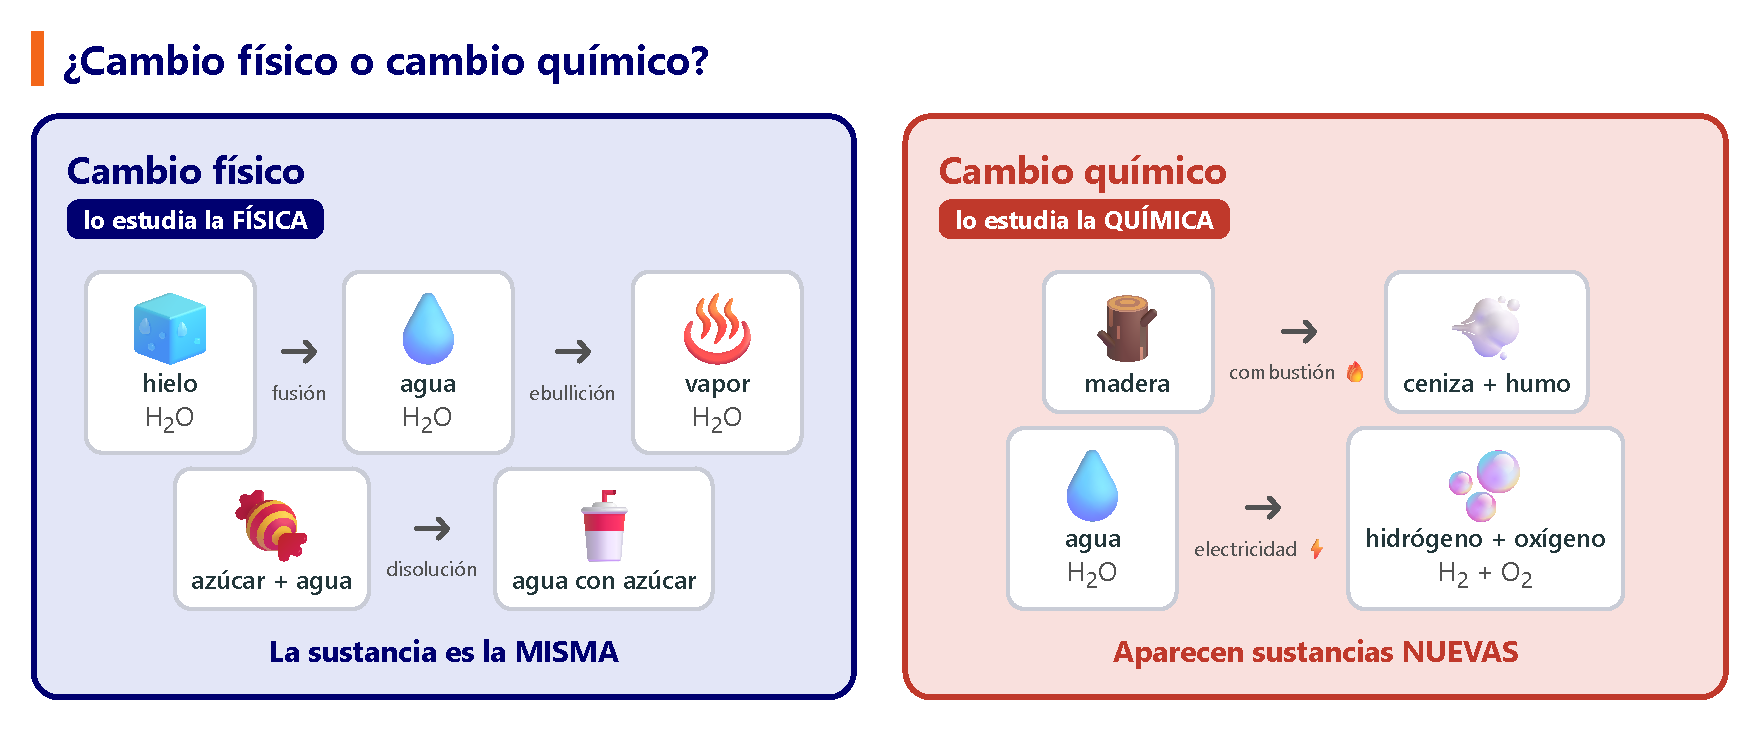
\includegraphics[width=\textwidth]{FigurasSVG/Unit_1_Matter_Measurement/pdf/physical_chemical_es.pdf}
    \caption{En un cambio físico la sustancia es la misma; en un cambio químico se forman sustancias nuevas.}
    \label{fig:u1_physical_chemical}
\end{figure}

\begin{impt}
    \textbf{Prueba rápida}: pregúntate «\emph{¿al final sigue siendo la misma sustancia?}». Si la respuesta es \textbf{sí} \(\to\) cambio físico. Si es \textbf{no} \(\to\) cambio químico.
\end{impt}

\begin{exercise}
    Clasifica estos ejemplos como cambios \textbf{físicos} o \textbf{químicos}:
    \begin{enumerate}[label=\letraminuscula]
        \item Disolver azúcar en agua.
        \item Quemar madera.
        \item Triturar alimentos.
        \item Modelar un trozo de arcilla.
        \item Derretir un helado.
        \item Freír un filete.
    \end{enumerate}
    \begin{solu}
        \begin{enumerate}[label=\alph*)]
            \item Físico (el azúcar sigue siendo azúcar, solo que mezclado con agua).
            \item Químico (aparecen sustancias nuevas, como la ceniza y el humo).
            \item Físico (los alimentos cambian de forma, no de composición).
            \item Físico (solo cambia la forma).
            \item Físico (cambio de estado, de sólido a líquido).
            \item Químico (la composición del alimento cambia al cocinarlo).
        \end{enumerate}
    \end{solu}
\end{exercise}

\begin{exercise}
    Clasifica estos términos como \textbf{cuerpos} o \textbf{sistemas materiales}:

    Libro, móvil, aluminio, zumo, aire, atmósfera, botella de agua, pájaro, Luna.
    \begin{solu}
        \textbf{Cuerpos}: libro, móvil, botella de agua, pájaro, Luna (tienen límites definidos). \\
        \textbf{Sistemas materiales}: aluminio, zumo, aire, atmósfera (no tienen límites definidos propios).
    \end{solu}
\end{exercise}

\begin{exercise}
    Indica si cada situación la estudiaría la física o la química, y explica por qué:
    \begin{enumerate}[label=\letraminuscula]
        \item Una barra de metal que se alarga al calentarla.
        \item Un clavo que se oxida después de dejarlo fuera bajo la lluvia.
        \item Una pelota que rueda por una rampa.
        \item La leche que se agria y forma yogur.
    \end{enumerate}
    \begin{solu}
        \begin{enumerate}[label=\alph*)]
            \item Física: la barra sigue siendo el mismo metal, solo cambia su tamaño.
            \item Química: el óxido (óxido de hierro) es una sustancia nueva, distinta del hierro.
            \item Física: la composición de la pelota no cambia, solo su posición y su velocidad.
            \item Química: el yogur es una sustancia distinta de la leche.
        \end{enumerate}
    \end{solu}
\end{exercise}

\subsection{Las propiedades de la materia}

\begin{definition}[Propiedad de la materia]
    Es cualquier aspecto de la materia que podemos observar o medir.
\end{definition}

Clasificamos las propiedades respondiendo a tres preguntas:

\begin{figure}[H]
    \centering
    % [FIGURA ORIGINAL] \includegraphics[width=\textwidth]{Unit_1/properties_map}
    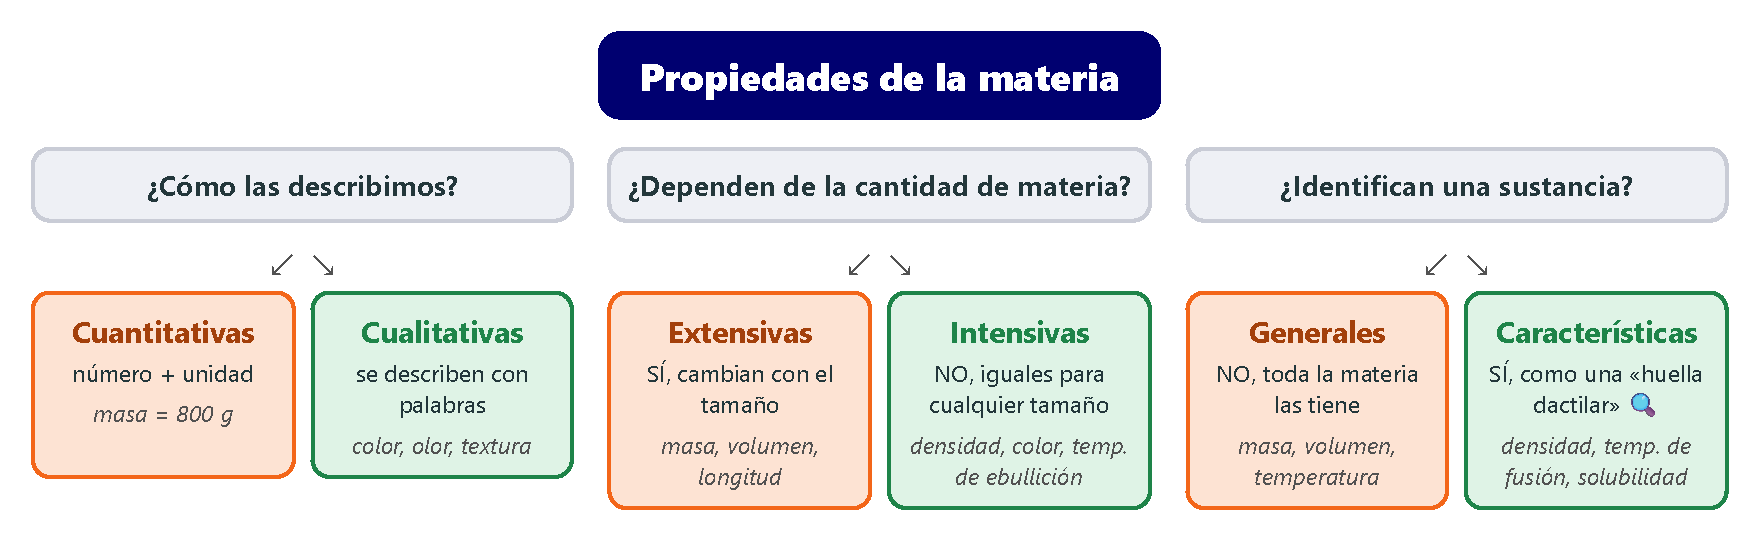
\includegraphics[width=\textwidth]{FigurasSVG/Unit_1_Matter_Measurement/pdf/properties_map_es.pdf}
    \caption{Tres formas de clasificar las propiedades de la materia.}
    \label{fig:u1_properties_map}
\end{figure}

Estas tres preguntas son \textbf{independientes}, así que hay que responder a \textbf{las tres} para cada propiedad. Dicho de otro modo, una \textbf{misma propiedad} es, a la vez, de un tipo en cada clasificación:

\begin{table}[H]
    \centering
    \small
    \renewcommand{\arraystretch}{1.35}
    \begin{tabular}{p{2.4cm}p{3.2cm}p{3.4cm}p{3.4cm}}
        \toprule
        \textbf{Propiedad} & \textbf{¿Cómo la describimos?} & \textbf{¿Depende de la cantidad?} & \textbf{¿Identifica una sustancia?} \\
        \midrule
        Masa & cuantitativa & extensiva & general \\
        Volumen & cuantitativa & extensiva & general \\
        Temperatura & cuantitativa & intensiva & general \\
        Densidad & cuantitativa & intensiva & característica \\
        Temperatura de ebullición & cuantitativa & intensiva & característica \\
        Color & cualitativa & intensiva & característica \\
        \bottomrule
    \end{tabular}
    \caption{Cada propiedad se clasifica de las tres formas a la vez.}
    \label{tab:u1_three_classifications}
\end{table}

\begin{impt}
    Una propiedad nunca es «solo» cuantitativa o «solo» intensiva. Por ejemplo, la \textbf{densidad} es \textbf{cuantitativa} (\qty{1.00}{\g\per\mL}), \textbf{intensiva} (una gota de agua y una piscina tienen la misma densidad) y \textbf{característica} (nos ayuda a identificar el agua).
\end{impt}

Las \negsubro{propiedades características} son la «huella dactilar» de una sustancia: nos ayudan a identificarla.

\begin{table}[H]
    \centering
    \small
    \renewcommand{\arraystretch}{1.35}
    \begin{tabular}{p{2.2cm}p{3.8cm}p{3.0cm}p{3.2cm}}
        \toprule
        \textbf{Propiedad} & \textbf{Qué nos dice} & \textbf{Tipo} & \textbf{Ejemplo} \\
        \midrule
        Densidad & masa que hay en cada unidad de volumen, \(d = m/V\) & cuantitativa, intensiva, característica & agua: \qty{1.00}{\g\per\mL} \\
        Temperatura de fusión & temperatura a la que funde un sólido & cuantitativa, intensiva, característica & hielo: \qty{0}{\celsius} \\
        Temperatura de ebullición & temperatura a la que hierve un líquido & cuantitativa, intensiva, característica & agua: \qty{100}{\celsius} \\
        Solubilidad & cuánto se disuelve en \qty{100}{\g} de agua & cuantitativa, intensiva, característica & azúcar: sí; aceite: no \\
        Conductividad & si deja pasar el calor y la electricidad & cuantitativa, intensiva, característica & metales: sí; madera: no \\
        Dureza & resistencia a ser rayado (escala del 1 al 10) & cuantitativa, intensiva, característica & talco: 1; diamante: 10 \\
        \bottomrule
    \end{tabular}
    \caption{Propiedades características de la materia.}
    \label{tab:u1_characteristic}
\end{table}

\begin{exercise}
    Clasifica cada propiedad de las \textbf{tres} formas: \textbf{cualitativa} o \textbf{cuantitativa}, \textbf{extensiva} o \textbf{intensiva}, y \textbf{general} o \textbf{característica}.
    \begin{enumerate}[label=\letraminuscula]
        \item La longitud.
        \item El olor.
        \item La temperatura de fusión.
        \item El peso.
        \item La dureza.
        \item El brillo de un metal.
        \item La conductividad eléctrica.
        \item El sabor.
    \end{enumerate}
    \begin{solu}
        \begin{enumerate}[label=\alph*)]
            \item Cuantitativa, extensiva, general.
            \item Cualitativa, intensiva, característica.
            \item Cuantitativa, intensiva, característica.
            \item Cuantitativa, extensiva, general.
            \item Cuantitativa, intensiva, característica.
            \item Cualitativa, intensiva, característica.
            \item Cuantitativa, intensiva, característica.
            \item Cualitativa, intensiva, característica.
        \end{enumerate}
    \end{solu}
\end{exercise}

\begin{exercise}
    Lucía describe su anillo de oro. Indica qué propiedad describe cada frase y \textbf{todos} sus tipos (cada propiedad tiene un tipo en cada una de las tres clasificaciones):
    \begin{enumerate}[label=\letraminuscula]
        \item «El anillo tiene una masa de \qty{6}{\g}».
        \item «El oro es amarillo y brillante».
        \item «El oro funde a \qty{1064}{\celsius}».
        \item «El anillo ocupa \qty{0.31}{\mL}».
        \item «La densidad del oro es \qty{19.3}{\g\per\mL}».
        \item «El anillo está a \qty{36}{\celsius} porque lo llevo puesto».
    \end{enumerate}
    \begin{solu}
        \begin{enumerate}[label=\alph*)]
            \item Masa: cuantitativa, extensiva, general.
            \item Color y brillo: cualitativas, intensivas, características.
            \item Temperatura de fusión: cuantitativa, intensiva, característica.
            \item Volumen: cuantitativa, extensiva, general.
            \item Densidad: cuantitativa, intensiva, característica.
            \item Temperatura: cuantitativa, intensiva, general.
        \end{enumerate}
    \end{solu}
\end{exercise}



%----------------------------------------------------------------------------------------

\section{La medida}

% Unidad tachada (en rojo) para los factores de conversión de esta sección
\providecommand{\cancelunit}[1]{\cancelred{\unit{#1}}}

\begin{definition}[Magnitud]
    Es cualquier propiedad de la materia que se puede medir.
\end{definition}

\begin{definition}[Unidad]
    Es una cantidad conocida de una magnitud que se usa como referencia para medir esa magnitud.
\end{definition}

Para medir una magnitud, la comparamos con una unidad para saber cuántas veces contiene esa unidad. El resultado es un \textbf{número} (la cantidad) seguido de una \textbf{unidad}.

\begin{example}
    Longitud de una pila = \qty{5.0}{\cm}. Aquí, \(\num{5.0}\) es la cantidad y \(\unit{\cm}\) es la unidad.
\end{example}

\subsection{El Sistema Internacional de Unidades (SI)}

El \negsubro{Sistema Internacional de Unidades (SI)} establece, para cada magnitud, una unidad, sus múltiplos y sus submúltiplos, además de las normas para escribirlos correctamente.

\begin{itemize}
    \item El símbolo de una unidad se escribe en minúscula, salvo cuando procede del nombre de una persona (J de julio).
    \item El símbolo del múltiplo o submúltiplo se escribe \textbf{delante} de la unidad: km, cL.
    \item Los símbolos nunca llevan «s» de plural: escribimos \textbf{8 km}, no 8 kms.
    \item Siempre hay un espacio entre el número y la unidad: \textbf{8 m}, no 8m.
\end{itemize}

\begin{didyouknow}
    En 1999 la NASA perdió la \emph{Mars Climate Orbiter}, una sonda que costaba más de 100 millones de euros, porque un equipo usó unidades del SI (newtons) y otro usó unidades británicas (libras). La sonda se acercó demasiado a Marte y se destruyó. ¡Las unidades importan!
\end{didyouknow}

\begin{exercise}
    Indica si cada una de estas expresiones está escrita \textbf{correcta} o \textbf{incorrectamente} según las normas del SI, y corrige los errores: «5 Kg», «12 kms», «3 J», «8m».
    \begin{solu}
        \begin{itemize}
            \item «5 Kg» \(\to\) incorrecta, el símbolo del kilogramo va en minúscula: \textbf{5 kg}.
            \item «12 kms» \(\to\) incorrecta, los símbolos nunca llevan «s» de plural: \textbf{12 km}.
            \item «3 J» \(\to\) correcta, la J (julio) va en mayúscula porque procede del nombre de una persona (Joule).
            \item «8m» \(\to\) incorrecta, tiene que haber un espacio entre el número y la unidad: \textbf{8 m}.
        \end{itemize}
    \end{solu}
\end{exercise}

\begin{exercise}
    Explica por qué el SI es útil para los científicos de todo el mundo, aunque hablen idiomas distintos. Pon un ejemplo de un problema que podría ocurrir si dos países usaran unidades distintas para la misma magnitud.
    \begin{solu}
        El SI da un único conjunto de unidades y símbolos, acordado por todos, para cada magnitud, así que científicos de países distintos pueden compartir y entender los datos sin confusiones y sin tener que traducir unidades. \\
        Por ejemplo, si un equipo mide una distancia en millas y otro la lee como si fueran kilómetros, obtendría un valor muy distinto (y erróneo), lo que podría provocar errores graves, como que una sonda espacial no llegue a su destino.
    \end{solu}
\end{exercise}

%----------------------------------------------------------------------------------------

\subsection{Magnitudes fundamentales y derivadas}

No todas las magnitudes son igual de «básicas». Algunas son los ladrillos con los que se construyen todas las demás.

\begin{definition}[Magnitud fundamental]
    Es una magnitud que se define por sí misma, sin usar otras magnitudes. El SI elige \textbf{siete} magnitudes fundamentales, y cada una tiene su propia unidad.
\end{definition}

\begin{definition}[Magnitud derivada]
    Es una magnitud que se obtiene combinando magnitudes fundamentales mediante multiplicaciones o divisiones. Su unidad también se obtiene combinando las unidades de esas magnitudes fundamentales.
\end{definition}

\begin{figure}[H]
    \centering
    % [FIGURA ORIGINAL] \includegraphics[width=\textwidth]{Unit_1/fundamental_derived}
    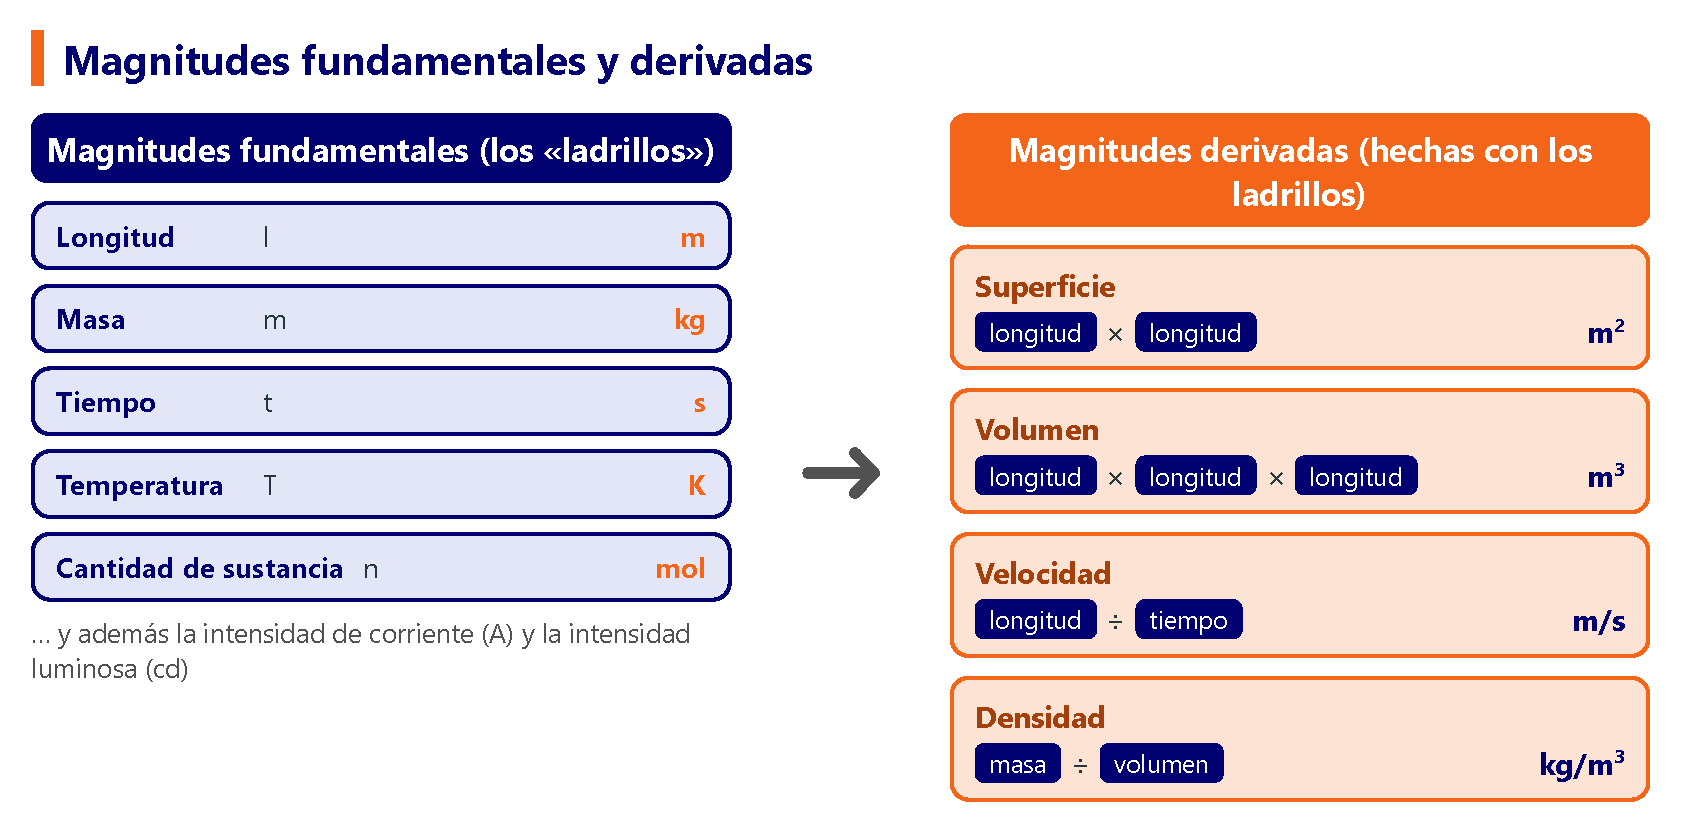
\includegraphics[width=\textwidth]{FigurasSVG/Unit_1_Matter_Measurement/pdf/fundamental_derived_es.pdf}
    \caption{Las magnitudes fundamentales son los «ladrillos» con los que se construyen las magnitudes derivadas.}
    \label{fig:u1_fundamental_derived}
\end{figure}

\begin{table}[H]
    \centering
    \small
    \renewcommand{\arraystretch}{1.35}
    \begin{tabular}{p{2.6cm}cp{3.9cm}p{2.3cm}c}
        \toprule
        \textbf{Magnitud} & \textbf{Símbolo} & \textbf{Unidades más usadas} & \textbf{Símbolos de las unidades} & \textbf{Unidad del SI} \\
        \midrule
        Longitud & \(l\) & kilómetro, metro, centímetro, milímetro & \unit{\km}, \unit{\m}, \unit{\cm}, \unit{\mm} & metro (\unit{\m}) \\
        Masa & \(m\) & tonelada, kilogramo, gramo, miligramo & \unit{\tonne}, \unit{\kg}, \unit{\g}, \unit{\mg} & kilogramo (\unit{\kg}) \\
        Tiempo & \(t\) & día, hora, minuto, segundo & \unit{\day}, \unit{\hour}, \unit{\minute}, \unit{\s} & segundo (\unit{\s}) \\
        Temperatura & \(T\) & grado Celsius, kelvin & \unit{\celsius}, \unit{\K} & kelvin (\unit{\K}) \\
        Cantidad de sustancia & \(n\) & mol, milimol & \unit{\mol}, \unit{\milli\mol} & mol (\unit{\mol}) \\
        Intensidad de corriente & \(I\) & amperio, miliamperio & \unit{\A}, \unit{\mA} & amperio (\unit{\A}) \\
        Intensidad luminosa & \(I_{v}\) & candela & \unit{\candela} & candela (\unit{\candela}) \\
        \bottomrule
    \end{tabular}
    \caption{Magnitudes fundamentales y sus unidades más usadas.}
    \label{tab:u1_fundamental}
\end{table}

\begin{table}[H]
    \centering
    \small
    \renewcommand{\arraystretch}{1.35}
    \begin{tabular}{p{2.6cm}cp{3.9cm}p{2.3cm}c}
        \toprule
        \textbf{Magnitud} & \textbf{Símbolo} & \textbf{Unidades más usadas} & \textbf{Símbolos de las unidades} & \textbf{Unidad del SI} \\
        \midrule
        Superficie \newline (longitud \(\times\) longitud) & \(S\) & kilómetro cuadrado, hectárea, metro cuadrado, centímetro cuadrado & \unit{\square\km}, \unit{\hectare}, \unit{\square\m}, \unit{\square\cm} & \unit{\square\m} \\
        Volumen \newline (longitud\(^3\)) & \(V\) & metro cúbico, centímetro cúbico, litro, mililitro & \unit{\cubic\m}, \unit{\cubic\cm}, \unit{\litre}, \unit{\mL} & \unit{\cubic\m} \\
        Densidad \newline (masa \(\div\) volumen) & \(d\) & kilogramo por metro cúbico, gramo por mililitro, gramo por litro & \unit{\kg\per\cubic\m}, \unit{\g\per\mL}, \unit{\g\per\litre} & \unit{\kg\per\cubic\m} \\
        Velocidad \newline (longitud \(\div\) tiempo) & \(v\) & kilómetro por hora, metro por segundo & \unit{\km\per\hour}, \unit{\m\per\s} & \unit{\m\per\s} \\
        Fuerza & \(F\) & newton, kilopondio & \unit{\N}, \unit{\kp} & newton (\unit{\N}) \\
        Presión & \(p\) & pascal, atmósfera, milímetro de mercurio & \unit{\Pa}, \unit{\atmospher}, \unit{\mmhg} & pascal (\unit{\Pa}) \\
        Energía & \(E\) & julio, caloría, kilocaloría, kilovatio hora & \unit{\J}, \unit{\calorie}, \unit{\kilo\calorie}, \unit{\kwh} & julio (\unit{\J}) \\
        \bottomrule
    \end{tabular}
    \caption{Algunas magnitudes derivadas y sus unidades más usadas.}
    \label{tab:u1_derived}
\end{table}

\begin{impt}
    Fíjate en que el símbolo de una \textbf{magnitud} se escribe en \textit{cursiva} (\(m\), \(V\), \(t\)) y el símbolo de una \textbf{unidad} en letra redonda (\unit{\m}, \unit{\litre}, \unit{\s}). No confundas \(m\) (la magnitud \emph{masa}) con \unit{\m} (la unidad \emph{metro}).
\end{impt}

\begin{exercise}
    Clasifica cada magnitud como \textbf{fundamental} o \textbf{derivada}, y escribe su unidad del SI: masa, velocidad, tiempo, superficie, temperatura, densidad, longitud, volumen.
    \begin{solu}
        \textbf{Fundamentales}: masa (\unit{\kg}), tiempo (\unit{\s}), temperatura (\unit{\K}), longitud (\unit{\m}). \\
        \textbf{Derivadas}: velocidad (\unit{\m\per\s}), superficie (\unit{\square\m}), densidad (\unit{\kg\per\cubic\m}), volumen (\unit{\cubic\m}).
    \end{solu}
\end{exercise}

\begin{exercise}
    La unidad de densidad del SI es el \unit{\kg\per\cubic\m}. Explica, usando las magnitudes fundamentales, de dónde sale esta unidad.
    \begin{solu}
        La densidad es la masa dividida entre el volumen, \(d = m/V\). La masa se mide en \unit{\kg}, y el volumen es longitud \(\times\) longitud \(\times\) longitud, así que se mide en \(\unit{\m}\cdot\unit{\m}\cdot\unit{\m} = \unit{\cubic\m}\). Dividiendo las dos unidades: \unit{\kg\per\cubic\m}.
    \end{solu}
\end{exercise}

%----------------------------------------------------------------------------------------

\subsection{Múltiplos y submúltiplos}

Los objetos que estudiamos pueden ser diminutos (una bacteria) o enormes (la Tierra). Si siempre usáramos la unidad básica, tendríamos que escribir números llenos de ceros, difíciles de leer y en los que es fácil equivocarse. Para evitarlo, el SI añade un \negsubro{prefijo} delante de la unidad.

\begin{definition}[Múltiplo y submúltiplo]
    Un \textbf{múltiplo} es una unidad mayor que la unidad básica (el \unit{\km} es \(10^{3}\) veces mayor que el \unit{\m}). Un \textbf{submúltiplo} es una unidad menor que la unidad básica (el \unit{\mm} es \(10^{3}\) veces menor que el \unit{\m}). Cada uno se nombra añadiendo un \textbf{prefijo} a la unidad básica, y cada prefijo vale una \textbf{potencia de 10}.
\end{definition}

\begin{figure}[H]
    \centering
    % [FIGURA ORIGINAL] \includegraphics[width=\textwidth]{Unit_1/prefix_scale}
    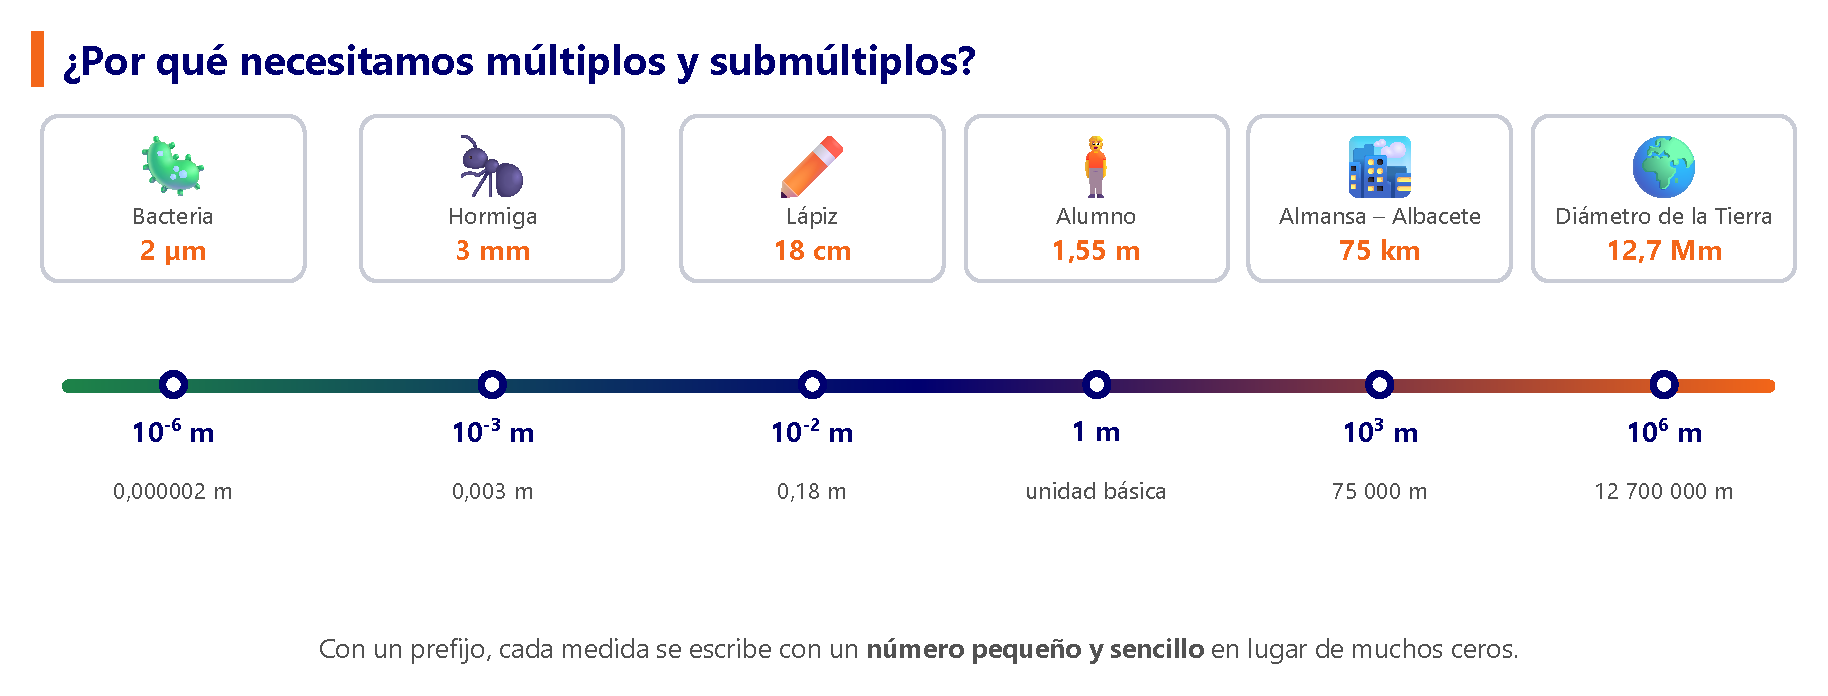
\includegraphics[width=\textwidth]{FigurasSVG/Unit_1_Matter_Measurement/pdf/prefix_scale_es.pdf}
    \caption{Con los prefijos, las longitudes muy pequeñas y muy grandes se escriben con números sencillos.}
    \label{fig:u1_prefix_scale}
\end{figure}

\begin{table}[H]
    \centering
    \small
    \renewcommand{\arraystretch}{1.3}
    \begin{tabular}{ccccrl}
        \toprule
         & \textbf{Prefijo} & \textbf{Símbolo} & \textbf{Potencia de 10} & \textbf{Valor decimal} & \textbf{Ejemplo} \\
        \midrule
        \multirow{5}{*}{\rotatebox{90}{\textbf{Múltiplos}}}
         & giga & G & \(10^{9}\) & \num{1000000000} & \qty{1}{\giga\byte} (memoria) \\
         & mega & M & \(10^{6}\) & \num{1000000} & \qty{1}{\mega\m} \\
         & kilo & k & \(10^{3}\) & \num{1000} & \qty{1}{\km}, \qty{1}{\kg} \\
         & hecto & h & \(10^{2}\) & \num{100} & \qty{1}{\hecto\litre} \\
         & deca & da & \(10^{1}\) & \num{10} & \qty{1}{\deca\gram} \\
        \midrule
        \multicolumn{3}{c}{\textbf{Unidad básica}} & \(10^{0}\) & \num{1} & \unit{\m}, \unit{\g}, \unit{\litre}, \unit{\s} \\
        \midrule
        \multirow{5}{*}{\rotatebox{90}{\textbf{Submúltiplos}}}
         & deci & d & \(10^{-1}\) & \num{0.1} & \qty{1}{\deci\litre} \\
         & centi & c & \(10^{-2}\) & \num{0.01} & \qty{1}{\cm} \\
         & mili & m & \(10^{-3}\) & \num{0.001} & \qty{1}{\mm}, \qty{1}{\mg} \\
         & micro & \(\upmu\) & \(10^{-6}\) & \num{0.000001} & \qty{1}{\um} (bacteria) \\
         & nano & n & \(10^{-9}\) & \num{0.000000001} & \qty{1}{\nm} (virus) \\
        \bottomrule
    \end{tabular}
    \caption{Múltiplos y submúltiplos de las unidades.}
    \label{tab:u1_prefixes}
\end{table}

\begin{impt}
    \negsubro{¿Por qué son tan importantes los múltiplos y submúltiplos?}
    \begin{itemize}
        \item Nos permiten escribir cualquier medida con un \textbf{número sencillo}: \qty{75}{\km} es mucho más claro que \qty{75000}{\m}, y \qty{2}{\um} es mucho más claro que \qty{0.000002}{\m}.
        \item Como cada prefijo es una \textbf{potencia de 10}, pasar de uno a otro es muy fácil: solo hay que mover la coma decimal.
        \item Los mismos prefijos sirven para \textbf{todas} las unidades: \unit{\km}, \unit{\kg}, \unit{\kilo\litre}, \unit{\kilo\joule}\ldots
    \end{itemize}
\end{impt}

Las unidades de longitud, masa y capacidad se pueden ordenar como una escalera. Cada escalón vale \textbf{10}, así que para saber cuántas veces contiene una unidad a otra solo hay que \textbf{contar los escalones} que hay entre ellas.

\begin{figure}[H]
    \centering
    % [FIGURA ORIGINAL] \includegraphics[width=0.75\textwidth]{Unit_1/prefix_ladder}
    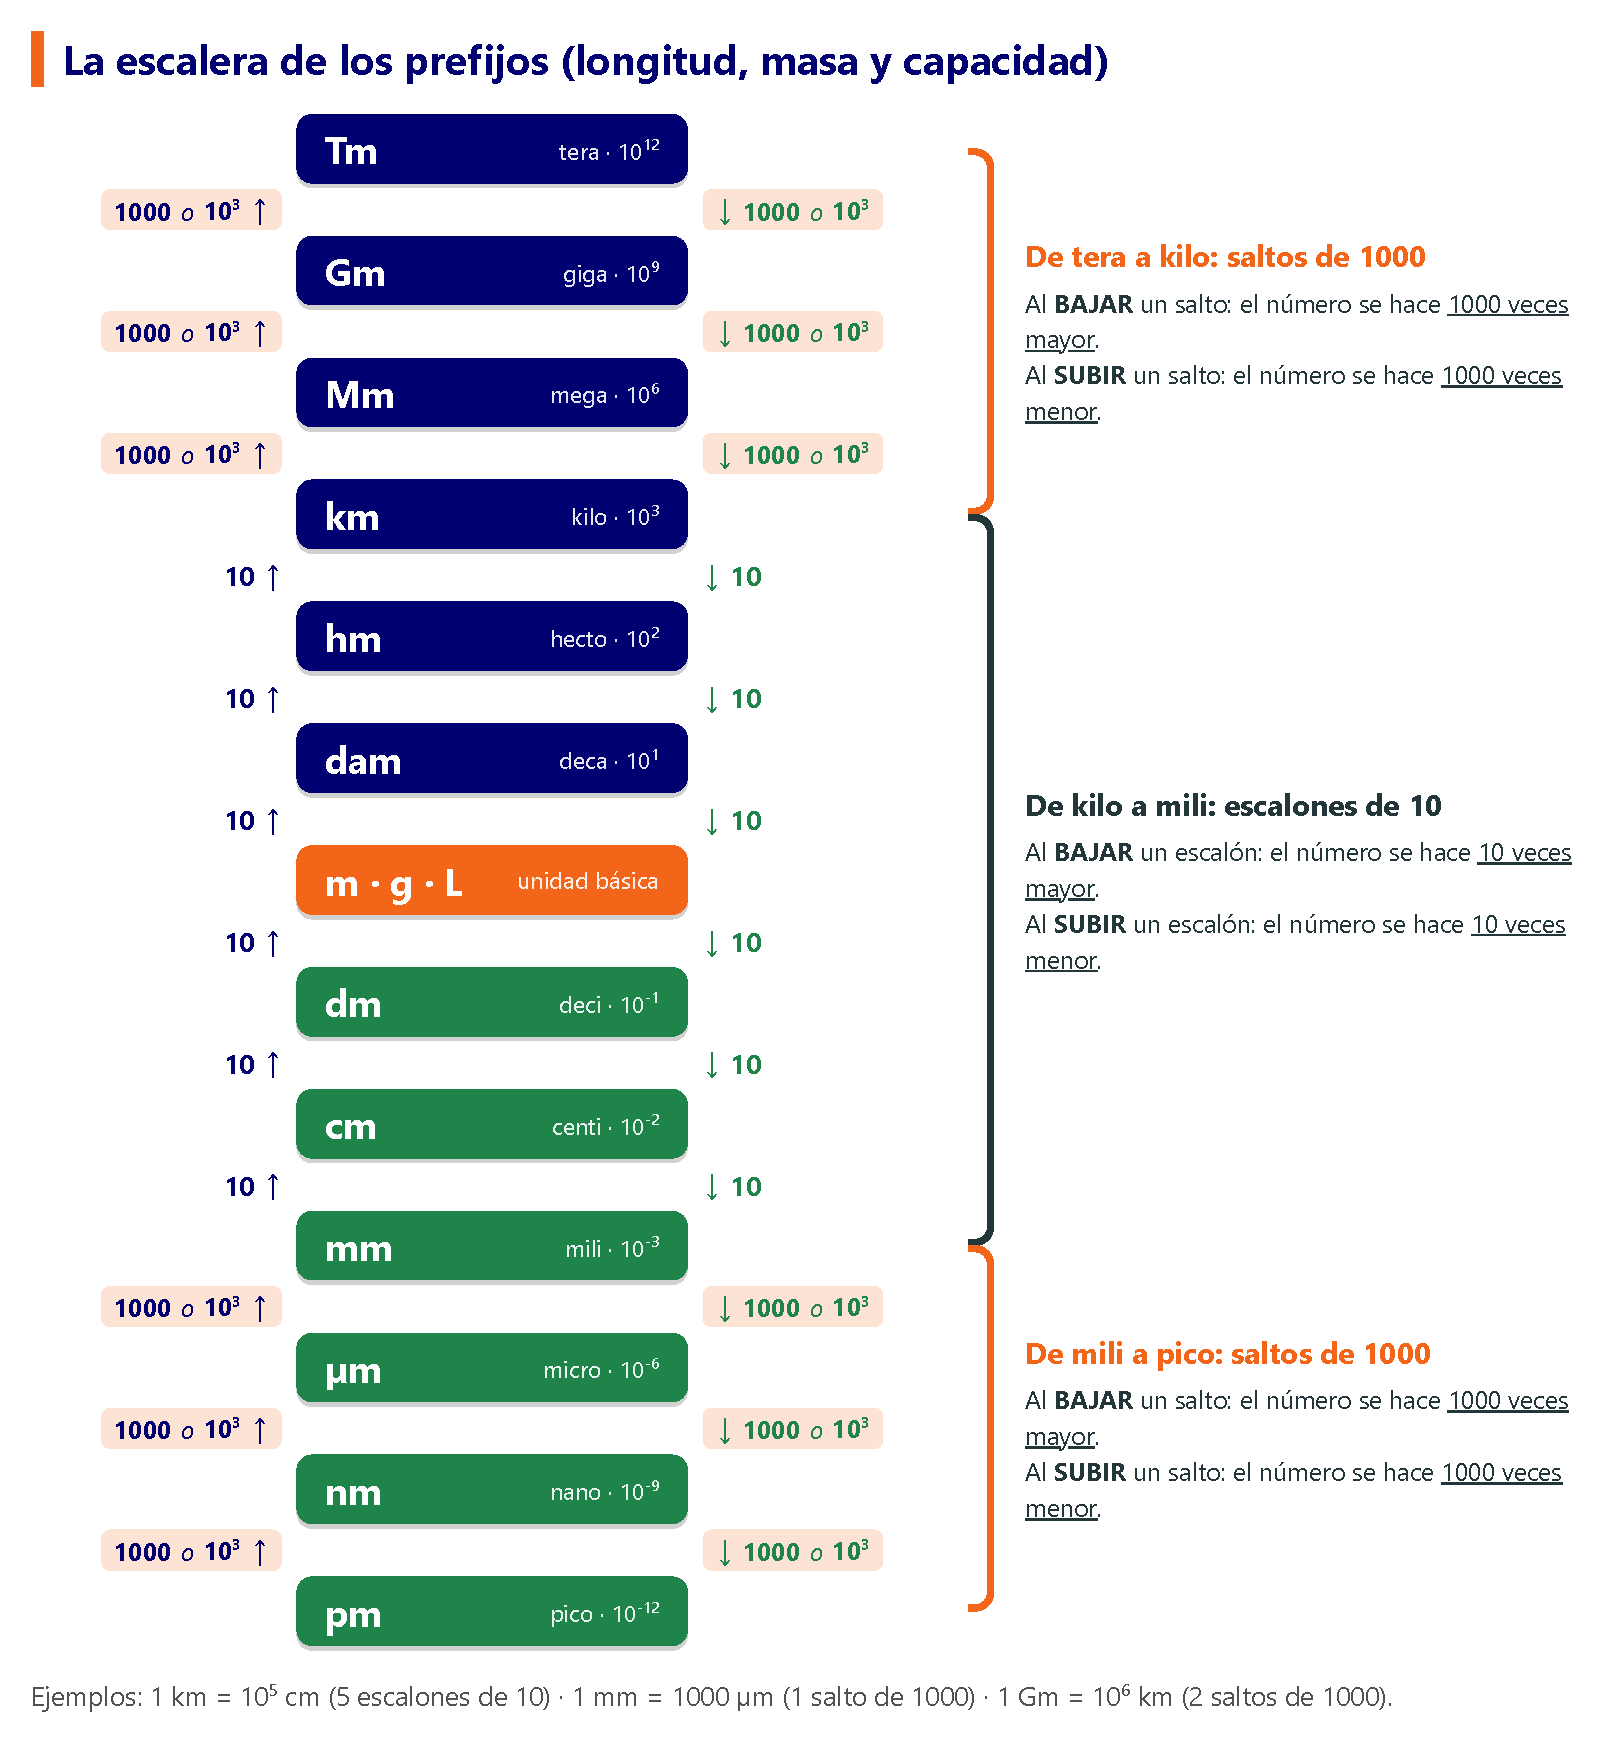
\includegraphics[width=0.75\textwidth]{FigurasSVG/Unit_1_Matter_Measurement/pdf/prefix_ladder_es.pdf}
    \caption{La escalera de los prefijos: cada escalón es una potencia de 10.}
    \label{fig:u1_prefix_ladder}
\end{figure}

\begin{example}
    Contando los escalones de la escalera:
    \begin{itemize}
        \item Del \unit{\km} al \unit{\m} hay 3 escalones: \(\qty{1}{\km} = \qty{e3}{\m}\).
        \item Del \unit{\m} al \unit{\cm} hay 2 escalones: \(\qty{1}{\m} = \qty{e2}{\cm}\).
        \item Del \unit{\kg} al \unit{\mg} hay 6 escalones: \(\qty{1}{\kg} = \qty{e6}{\mg}\).
        \item Del \unit{\deca\litre} al \unit{\centi\litre} hay 3 escalones: \(\qty{1}{\deca\litre} = \qty{e3}{\centi\litre}\).
    \end{itemize}
\end{example}

\begin{exercise}
    Escribe la equivalencia entre cada pareja de unidades, poniendo el \textbf{1} delante de la unidad mayor y usando una potencia de 10: \textbf{a)} \unit{\hecto\m} y \unit{\dm}; \textbf{b)} \unit{\g} y \unit{\mg}; \textbf{c)} \unit{\kilo\litre} y \unit{\mL}; \textbf{d)} \unit{\cm} y \unit{\mm}; \textbf{e)} \unit{\deca\gram} y \unit{\deci\gram}.
    \begin{solu}
        a) \(\qty{1}{\hecto\m} = \qty{e3}{\dm}\); b) \(\qty{1}{\g} = \qty{e3}{\mg}\); c) \(\qty{1}{\kilo\litre} = \qty{e6}{\mL}\); d) \(\qty{1}{\cm} = \qty{e1}{\mm} = \qty{10}{\mm}\); e) \(\qty{1}{\deca\gram} = \qty{e2}{\deci\gram}\).
    \end{solu}
\end{exercise}

\begin{exercise}
    Elige la unidad más adecuada para expresar cada medida: el grosor de una moneda, la distancia de Almansa a Madrid, la masa de un camión, la masa de un grano de arroz, el volumen de agua de una piscina, el volumen de una dosis de jarabe.
    \begin{solu}
        Grosor de una moneda: \unit{\mm}. Distancia Almansa--Madrid: \unit{\km}. Masa de un camión: \unit{\tonne} o \unit{\kg}. Masa de un grano de arroz: \unit{\mg}. Agua de una piscina: \unit{\cubic\m} o \unit{\kilo\litre}. Dosis de jarabe: \unit{\mL}.
    \end{solu}
\end{exercise}

\begin{impt}
    \negsubro{Cómo se lee una unidad (¡muy importante!)}

    Cuando miramos una unidad, la leemos siempre \textbf{de derecha a izquierda}:
    \begin{enumerate}[label=\numberballmDarkTeal]
        \item Primero buscamos el \textbf{símbolo de la unidad}: es la \textbf{última} letra (o letras) del símbolo.
        \item Después identificamos la \textbf{magnitud} que mide esa unidad: \unit{\m} \(\to\) longitud, \unit{\g} \(\to\) masa, \unit{\litre} \(\to\) capacidad, \unit{\s} \(\to\) tiempo\ldots
        \item Por último, miramos la letra que hay \textbf{delante de la unidad}: es el \textbf{prefijo}, y nos dice si es un \textbf{múltiplo} o un \textbf{submúltiplo}. Si no hay ninguna letra delante, es la unidad básica.
    \end{enumerate}
\end{impt}

\begin{figure}[H]
    \centering
    % [FIGURA ORIGINAL] \includegraphics[width=\textwidth]{Unit_1/read_unit}
    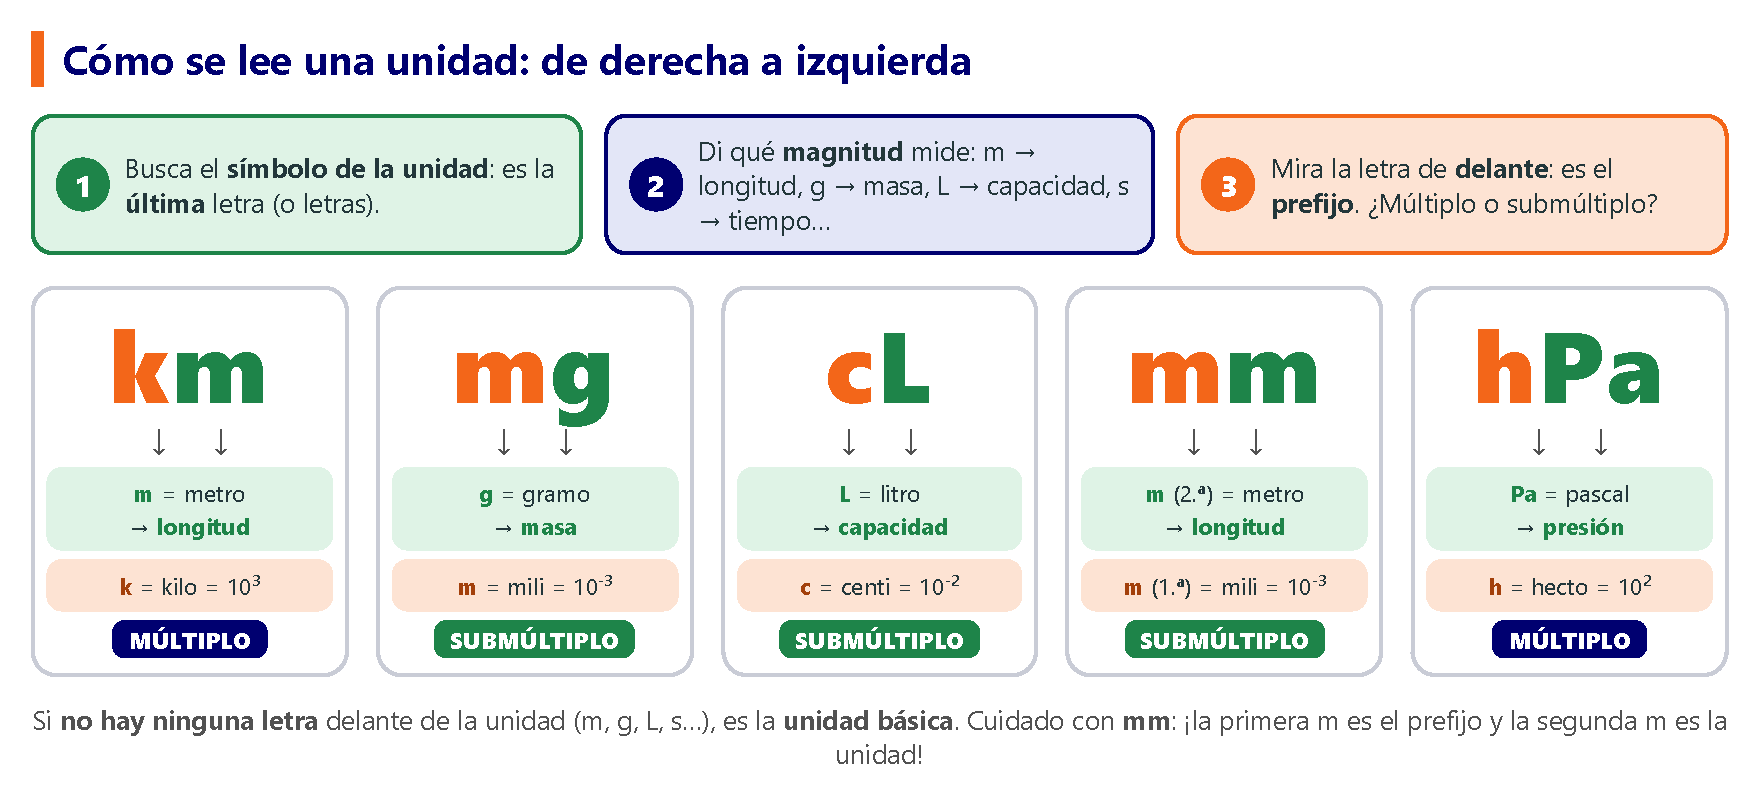
\includegraphics[width=\textwidth]{FigurasSVG/Unit_1_Matter_Measurement/pdf/read_unit_es.pdf}
    \caption{Una unidad se lee de derecha a izquierda: primero la unidad y su magnitud, después el prefijo.}
    \label{fig:u1_read_unit}
\end{figure}

\begin{exercise}
    Para cada unidad, indica qué magnitud mide, qué prefijo tiene y si es un múltiplo o un submúltiplo: \unit{\kg}, \unit{\mL}, \unit{\cm}, \unit{\hecto\litre}, \unit{\ms}, \unit{\mm}.
    \begin{solu}
        \unit{\kg}: masa, kilo, múltiplo. \unit{\mL}: capacidad, mili, submúltiplo. \unit{\cm}: longitud, centi, submúltiplo. \unit{\hecto\litre}: capacidad, hecto, múltiplo. \unit{\ms}: tiempo, mili, submúltiplo. \unit{\mm}: longitud, mili (la primera m), submúltiplo.
    \end{solu}
\end{exercise}

%----------------------------------------------------------------------------------------

\subsection{Cambio de unidades: factores de conversión}

Muy a menudo necesitamos expresar una medida en otra unidad: una receta en gramos cuando la báscula usa kilogramos, o una velocidad en \unit{\m\per\s} cuando el coche marca \unit{\km\per\hour}. En este libro cambiaremos siempre de unidades con \negsubro{factores de conversión}.

\begin{impt}
    \negsubro{¿Qué significa «cambiar de unidades»?}
    \begin{itemize}
        \item Un cambio de unidades es un cambio entre \textbf{distintas unidades de la misma magnitud}: \unit{\hour}, \unit{\minute} y \unit{\s} son todas unidades de \textbf{tiempo}, así que podemos pasar de una a otra.
        \item También es un cambio entre \textbf{múltiplos y submúltiplos} de la misma unidad: \unit{\km} \(\to\) \unit{\m} \(\to\) \unit{\cm}.
        \item \textbf{Nunca} podemos cambiar entre unidades de \textbf{magnitudes distintas}: los \unit{\km} nunca pueden convertirse en \unit{\kg}, porque la longitud y la masa son magnitudes distintas.
    \end{itemize}
    La medida no cambia: es la \textbf{misma cantidad}, solo que escrita con otra unidad.
\end{impt}

\begin{figure}[H]
    \centering
    % [FIGURA ORIGINAL] \includegraphics[width=\textwidth]{Unit_1/same_quantity}
    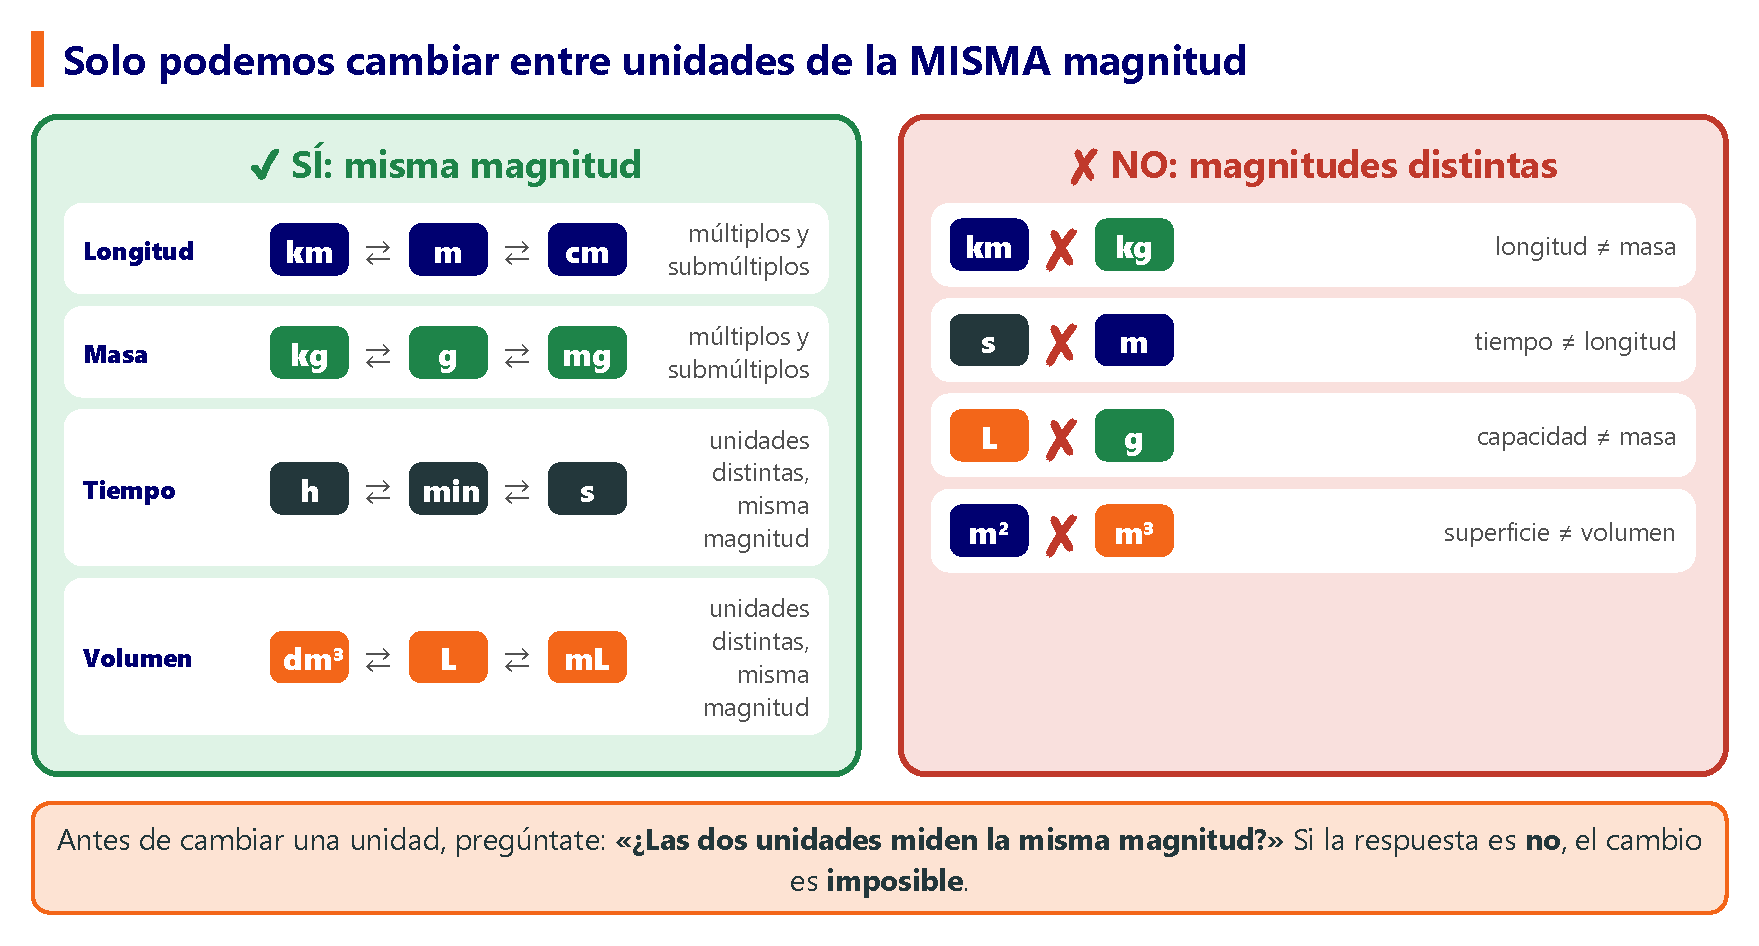
\includegraphics[width=\textwidth]{FigurasSVG/Unit_1_Matter_Measurement/pdf/same_quantity_es.pdf}
    \caption{Solo podemos cambiar entre unidades que miden la misma magnitud.}
    \label{fig:u1_same_quantity}
\end{figure}

\begin{definition}[Factor de conversión]
    Es una fracción cuyo numerador y denominador son la \textbf{misma cantidad}, escrita en \textbf{unidades distintas}. Por ejemplo,
    \(\dfrac{\qty{e3}{\m}}{\qty{1}{\km}}\) o \(\dfrac{\qty{1}{\km}}{\qty{e3}{\m}}\).
    Como arriba y abajo hay lo mismo, un factor de conversión vale exactamente \textbf{1}: multiplicar por él no cambia la cantidad, solo la unidad en la que está escrita.
\end{definition}

\begin{impt}
    \negsubro{Reglas de oro para escribir factores de conversión}
    \begin{enumerate}[label=\numberballmDarkTeal]
        \item En la equivalencia entre las dos unidades, el \textbf{1} va siempre con la \textbf{unidad mayor}: \(\qty{1}{\km} = \qty{e3}{\m}\) (nunca \(\qty{1}{\m} = \qty{e-3}{\km}\)); \(\qty{1}{\hour} = \qty{3600}{\s}\); \(\qty{1}{\atmospher} = \qty{760}{\mmhg}\).
        \item Entre múltiplos y submúltiplos, y siempre que los números sean muy grandes, usamos \textbf{potencias de 10}: \(\qty{1}{\kg} = \qty{e6}{\mg}\) en lugar de \(\qty{1}{\kg} = \qty{1000000}{\mg}\).
        \item La unidad que queremos \textbf{quitar} va en el \textbf{denominador}, y la unidad que queremos \textbf{obtener} va en el \textbf{numerador}.
    \end{enumerate}
\end{impt}

\begin{figure}[H]
    \centering
    % [FIGURA ORIGINAL] \includegraphics[width=0.95\textwidth]{Unit_1/conversion_factor}
    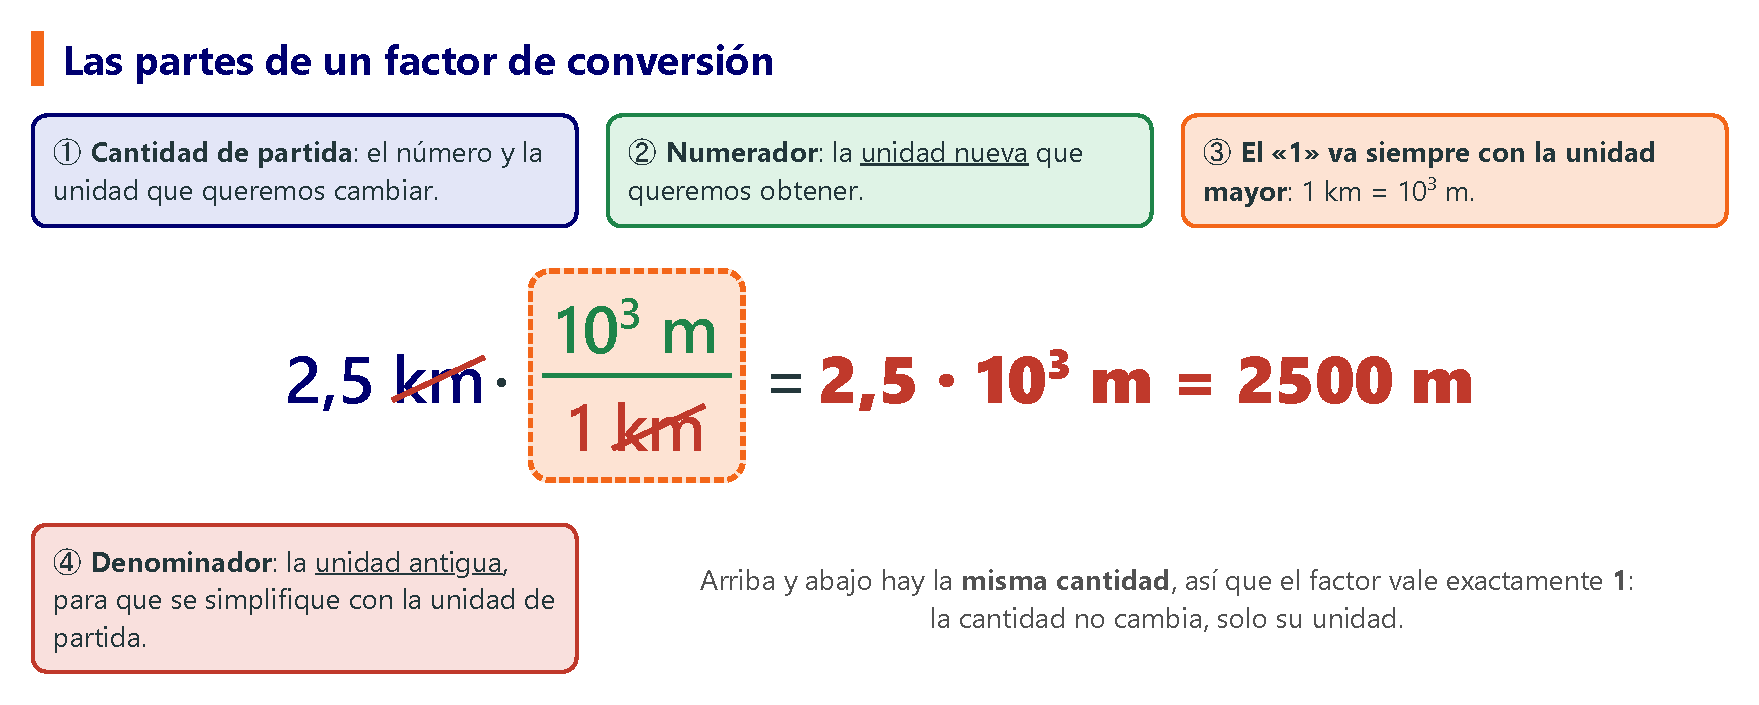
\includegraphics[width=0.95\textwidth]{FigurasSVG/Unit_1_Matter_Measurement/pdf/conversion_factor_es.pdf}
    \caption{Las partes de un factor de conversión.}
    \label{fig:u1_conversion_factor}
\end{figure}

\negsubro{Método, paso a paso}:
\begin{enumerate}[label=\numberballmDarkTeal]
    \item Escribe la cantidad que quieres cambiar (número y unidad).
    \item Escribe la \textbf{equivalencia} entre la unidad inicial y la final, con el 1 delante de la unidad mayor y usando potencias de 10.
    \item Construye el \textbf{factor de conversión} a partir de la equivalencia: la unidad inicial va en el denominador, para que se simplifique, y la unidad final va en el numerador.
    \item Multiplica, \textbf{simplifica} las unidades que aparecen arriba y abajo, y calcula.
    \item Escribe el resultado con su unidad (si tiene muchos ceros, déjalo como potencia de 10).
\end{enumerate}

Si no hay una equivalencia directa entre las dos unidades, podemos encadenar varios factores de conversión, uno detrás de otro, como los eslabones de una cadena.

%------------------------------------------------

\subsubsection{Unidades simples: longitud, masa y capacidad}

\begin{example}
    \textbf{Expresa \qty{0.8}{\km} en \unit{\dm}.}
    \begin{enumerate}[label=\numberballmDarkTeal]
        \item Cantidad: \qty{0.8}{\km}.
        \item Equivalencia (4 escalones en la escalera; el 1 va con el \unit{\km}): \(\qty{1}{\km} = \qty{e4}{\dm}\).
        \item La unidad que hay que quitar (\unit{\km}) va en el denominador.
        \item \(
            \num{0.8}\,\cancelunit{\km} \cdot \dfrac{\qty{e4}{\dm}}{1\,\cancelunit{\km}} = \qty{0.8e4}{\dm}
        \)
        \item \(\textcolor{red}{\qty{8000}{\dm}}\)
    \end{enumerate}
\end{example}

\begin{example}
    \textbf{Expresa \qty{850}{\deci\gram} en \unit{\hecto\gram}.} \\
    Equivalencia (3 escalones; el 1 va con el \unit{\hecto\gram}, que es mayor): \(\qty{1}{\hecto\gram} = \qty{e3}{\deci\gram}\).
    \begin{equation*}
        \num{850}\,\cancelunit{\deci\gram} \cdot \dfrac{\qty{1}{\hecto\gram}}{\num{e3}\,\cancelunit{\deci\gram}} = \qty{850e-3}{\hecto\gram} = \textcolor{red}{\qty{0.85}{\hecto\gram}}
    \end{equation*}
\end{example}

\begin{example}
    \textbf{Expresa \qty{2.5}{\litre} en \unit{\mL}.} \\
    Equivalencia: \(\qty{1}{\litre} = \qty{e3}{\mL}\).
    \begin{equation*}
        \num{2.5}\,\cancelunit{\litre} \cdot \dfrac{\qty{e3}{\mL}}{1\,\cancelunit{\litre}} = \qty{2.5e3}{\mL} = \textcolor{red}{\qty{2500}{\mL}}
    \end{equation*}
\end{example}

\begin{exercise}
    Cambia de unidades estas cantidades usando factores de conversión:
    \begin{enumerate}[label=\letraminuscula]
        \item \(\qty{25.8}{\g} \to \unit{\centi\gram}\)
        \item \(\qty{0.05}{\hecto\gram} \to \unit{\deci\gram}\)
        \item \(\qty{3.5}{\deca\gram} \to \unit{\kg}\)
        \item \(\qty{450}{\mg} \to \unit{\kg}\)
        \item \(\qty{1.2}{\km} \to \unit{\cm}\)
        \item \(\qty{330}{\mL} \to \unit{\litre}\)
    \end{enumerate}
    \begin{solu}
        \begin{enumerate}[label=\alph*)]
            \item \(\num{25.8}\,\unit{\g} \cdot \dfrac{\qty{e2}{\centi\gram}}{\qty{1}{\g}} = \qty{2580}{\centi\gram}\)
            \item \(\num{0.05}\,\unit{\hecto\gram} \cdot \dfrac{\qty{e3}{\deci\gram}}{\qty{1}{\hecto\gram}} = \qty{50}{\deci\gram}\)
            \item \(\num{3.5}\,\unit{\deca\gram} \cdot \dfrac{\qty{1}{\kg}}{\qty{e2}{\deca\gram}} = \qty{3.5e-2}{\kg} = \qty{0.035}{\kg}\)
            \item \(\num{450}\,\unit{\mg} \cdot \dfrac{\qty{1}{\kg}}{\qty{e6}{\mg}} = \qty{4.5e-4}{\kg} = \qty{0.00045}{\kg}\)
            \item \(\num{1.2}\,\unit{\km} \cdot \dfrac{\qty{e5}{\cm}}{\qty{1}{\km}} = \qty{1.2e5}{\cm} = \qty{120000}{\cm}\)
            \item \(\num{330}\,\unit{\mL} \cdot \dfrac{\qty{1}{\litre}}{\qty{e3}{\mL}} = \qty{0.33}{\litre}\)
        \end{enumerate}
    \end{solu}
\end{exercise}

\begin{exercise}
    Ordena estas cantidades de mayor a menor: \qty{0.015}{\kg}, \qty{2765}{\deci\gram}, \qty{2.54}{\deca\gram}.
    \begin{solu}
        Las pasamos todas a gramos: \\
        \(\num{0.015}\,\unit{\kg} \cdot \dfrac{\qty{e3}{\g}}{\qty{1}{\kg}} = \qty{15}{\g}\); \quad
        \(\num{2765}\,\unit{\deci\gram} \cdot \dfrac{\qty{1}{\g}}{\qty{e1}{\deci\gram}} = \qty{276.5}{\g}\); \quad
        \(\num{2.54}\,\unit{\deca\gram} \cdot \dfrac{\qty{e1}{\g}}{\qty{1}{\deca\gram}} = \qty{25.4}{\g}\). \\
        Orden: \(\qty{2765}{\deci\gram} > \qty{2.54}{\deca\gram} > \qty{0.015}{\kg}\).
    \end{solu}
\end{exercise}

\begin{exercise}
    Una receta necesita \qty{0.75}{\kg} de harina, pero la báscula de la cocina solo marca gramos. ¿Cuántos gramos hay que pesar? Si un paquete contiene \qty{2}{\kg} de harina, ¿cuántas recetas completas se pueden hacer con él?
    \begin{solu}
        \(\num{0.75}\,\unit{\kg} \cdot \dfrac{\qty{e3}{\g}}{\qty{1}{\kg}} = \qty{750}{\g}\). \\
        \(\qty{2}{\kg} = \qty{2000}{\g}\); número de recetas \(= 2000 / 750 \approx \num{2.67}\), así que se pueden hacer \textbf{2 recetas completas}.
    \end{solu}
\end{exercise}

\begin{exercise}
    Cambia de unidades estas cantidades usando factores de conversión:
    \begin{enumerate}[label=\letraminuscula]
        \item \(\qty{500}{\hecto\gram} \to \unit{\g}\)
        \item \(\qty{60}{\cm} \to \unit{\m}\)
        \item \(\qty{2000}{\hecto\m} \to \unit{\deca\m}\)
        \item \(\qty{5.7}{\kg} \to \unit{\g}\)
        \item \(\qty{300}{\dm} \to \unit{\hecto\m}\)
        \item \(\qty{563}{\km} \to \unit{\hecto\m}\)
        \item \(\qty{3}{\dm} \to \unit{\deca\m}\)
        \item \(\qty{7}{\dm} \to \unit{\cm}\)
        \item \(\qty{5}{\giga\m} \to \unit{\nano\m}\)
        \item \(\qty{26}{\micro\m} \to \unit{\km}\)
    \end{enumerate}
    \begin{solu}
        \begin{enumerate}[label=\alph*)]
            \item \(\num{500}\,\unit{\hecto\gram} \cdot \dfrac{\qty{e2}{\g}}{\qty{1}{\hecto\gram}} = \qty{5e4}{\g} = \qty{50000}{\g}\)
            \item \(\num{60}\,\unit{\cm} \cdot \dfrac{\qty{1}{\m}}{\qty{e2}{\cm}} = \qty{0.6}{\m}\)
            \item \(\num{2000}\,\unit{\hecto\m} \cdot \dfrac{\qty{e1}{\deca\m}}{\qty{1}{\hecto\m}} = \qty{2e4}{\deca\m}\)
            \item \(\num{5.7}\,\unit{\kg} \cdot \dfrac{\qty{e3}{\g}}{\qty{1}{\kg}} = \qty{5.7e3}{\g} = \qty{5700}{\g}\)
            \item \(\num{300}\,\unit{\dm} \cdot \dfrac{\qty{1}{\hecto\m}}{\qty{e3}{\dm}} = \qty{0.3}{\hecto\m}\)
            \item \(\num{563}\,\unit{\km} \cdot \dfrac{\qty{e1}{\hecto\m}}{\qty{1}{\km}} = \qty{5630}{\hecto\m}\)
            \item \(\num{3}\,\unit{\dm} \cdot \dfrac{\qty{1}{\deca\m}}{\qty{e2}{\dm}} = \qty{3e-2}{\deca\m} = \qty{0.03}{\deca\m}\)
            \item \(\num{7}\,\unit{\dm} \cdot \dfrac{\qty{e1}{\cm}}{\qty{1}{\dm}} = \qty{70}{\cm}\)
            \item \(\num{5}\,\unit{\giga\m} \cdot \dfrac{\qty{e9}{\m}}{\qty{1}{\giga\m}} \cdot \dfrac{\qty{e9}{\nano\m}}{\qty{1}{\m}} = \qty{5e18}{\nano\m}\)
            \item \(\num{26}\,\unit{\micro\m} \cdot \dfrac{\qty{1}{\m}}{\qty{e6}{\micro\m}} \cdot \dfrac{\qty{1}{\km}}{\qty{e3}{\m}} = \qty{26e-9}{\km} = \qty{2.6e-8}{\km}\)
        \end{enumerate}
    \end{solu}
\end{exercise}

%------------------------------------------------

\subsubsection{Superficie}

\begin{definition}[Superficie]
    Es una magnitud que se obtiene multiplicando dos longitudes expresadas en la misma unidad. Su unidad del SI es el metro cuadrado, \unit{\square\metre}.
\end{definition}

\begin{equation*}
    \qty{5.40}{\m} \cdot \qty{6.50}{\m} = \qty{35.10}{\square\metre}
\end{equation*}

Un cuadrado de \qty{1}{\m} \(\times\) \qty{1}{\m} se puede dividir en \(10 \times 10 = 100\) cuadraditos de \qty{1}{\dm} \(\times\) \qty{1}{\dm}. Así, mientras que \(\qty{1}{\m} = \qty{10}{\dm}\), tenemos que \(\qty{1}{\square\m} = \qty{e2}{\square\dm}\): \textbf{el factor de la longitud se eleva al cuadrado}.

\begin{figure}[H]
    \centering
    % [FIGURA ORIGINAL] \includegraphics[width=0.85\textwidth]{Unit_1/square_units}
    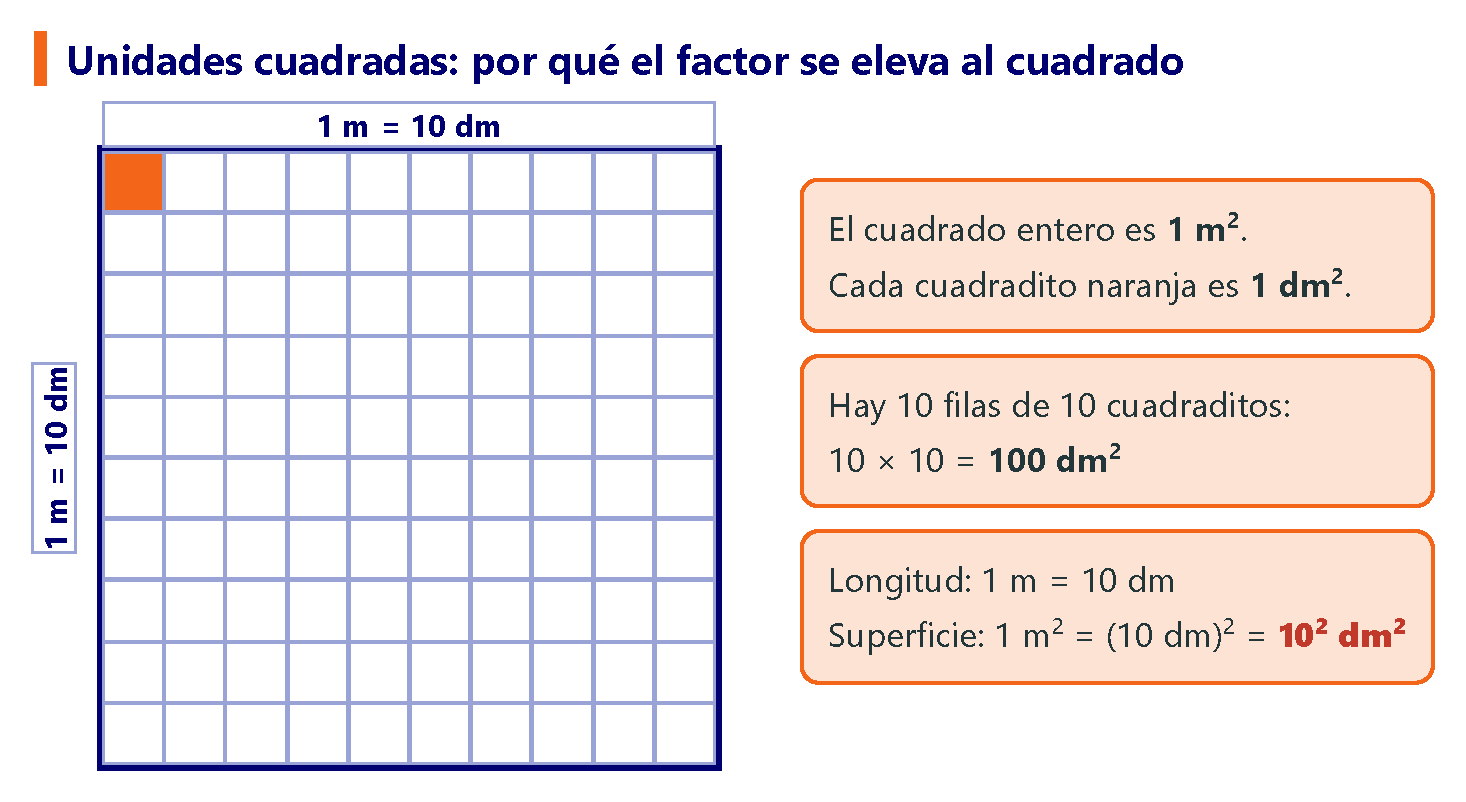
\includegraphics[width=0.85\textwidth]{FigurasSVG/Unit_1_Matter_Measurement/pdf/square_units_es.pdf}
    \caption{Un metro cuadrado contiene \(10^{2}\) decímetros cuadrados.}
    \label{fig:u1_square_units}
\end{figure}

\begin{impt}
    \negsubro{Truco para la superficie}: escribe el factor de conversión como si fuera un cambio de \textbf{longitud} (una unidad simple) y después \textbf{eleva todo el factor al cuadrado}.
    \begin{equation*}
        \text{Longitud: } \dfrac{\qty{e2}{\cm}}{\qty{1}{\m}}
        \quad\Longrightarrow\quad
        \text{Superficie: } \left(\dfrac{\qty{e2}{\cm}}{\qty{1}{\m}}\right)^{2} = \dfrac{\qty{e4}{\square\cm}}{\qty{1}{\square\m}}
    \end{equation*}
    Por tanto, cada escalón de la escalera de unidades de superficie vale \(10^{2} = 100\).
\end{impt}

\begin{table}[H]
    \centering
    \small
    \renewcommand{\arraystretch}{1.3}
    \begin{tabular}{cccc}
        \toprule
        \textbf{Unidad} & \textbf{Símbolo} & \textbf{Equivalencia con el \unit{\square\m}} & \textbf{Longitud equivalente} \\
        \midrule
        kilómetro cuadrado & \unit{\square\km} & \(\qty{1}{\square\km} = \qty{e6}{\square\m}\) & \(\qty{1}{\km} = \qty{e3}{\m}\) \\
        hectómetro cuadrado (hectárea) & \unit{\square\hecto\m} (\unit{\hectare}) & \(\qty{1}{\square\hecto\m} = \qty{e4}{\square\m}\) & \(\qty{1}{\hecto\m} = \qty{e2}{\m}\) \\
        decámetro cuadrado & \unit{\square\deca\m} & \(\qty{1}{\square\deca\m} = \qty{e2}{\square\m}\) & \(\qty{1}{\deca\m} = \qty{e1}{\m}\) \\
        \midrule
        metro cuadrado & \unit{\square\m} & unidad básica & unidad básica \\
        \midrule
        decímetro cuadrado & \unit{\square\dm} & \(\qty{1}{\square\m} = \qty{e2}{\square\dm}\) & \(\qty{1}{\m} = \qty{e1}{\dm}\) \\
        centímetro cuadrado & \unit{\square\cm} & \(\qty{1}{\square\m} = \qty{e4}{\square\cm}\) & \(\qty{1}{\m} = \qty{e2}{\cm}\) \\
        milímetro cuadrado & \unit{\square\mm} & \(\qty{1}{\square\m} = \qty{e6}{\square\mm}\) & \(\qty{1}{\m} = \qty{e3}{\mm}\) \\
        \bottomrule
    \end{tabular}
    \caption{Unidades de superficie.}
    \label{tab:u1_surface_units}
\end{table}

\begin{example}
    \textbf{Expresa \qty{0.5}{\square\deca\metre} en \unit{\square\dm}.}
    \begin{enumerate}[label=\numberballmDarkTeal]
        \item Cambio simple (longitud): \(\qty{1}{\deca\m} = \qty{e2}{\dm}\) \(\to\) factor \(\dfrac{\qty{e2}{\dm}}{\qty{1}{\deca\m}}\).
        \item Lo elevamos al cuadrado: \(\left(\dfrac{\qty{e2}{\dm}}{\qty{1}{\deca\m}}\right)^{2} = \dfrac{\qty{e4}{\square\dm}}{\qty{1}{\square\deca\m}}\).
        \item \(
            \num{0.5}\,\cancelunit{\square\deca\m} \cdot \dfrac{\qty{e4}{\square\dm}}{1\,\cancelunit{\square\deca\m}} = \qty{0.5e4}{\square\dm} = \textcolor{red}{\qty{5000}{\square\dm}}
        \)
    \end{enumerate}
\end{example}

\begin{example}
    \textbf{Expresa \qty{85}{\square\cm} en \unit{\square\m}.} \\
    Cambio simple: \(\qty{1}{\m} = \qty{e2}{\cm}\). Elevando el factor al cuadrado:
    \begin{equation*}
        \num{85}\,\cancelunit{\square\cm} \cdot \left(\dfrac{\qty{1}{\m}}{\num{e2}\,\cancelunit{\cm}}\right)^{2}
        = \num{85}\,\cancelunit{\square\cm} \cdot \dfrac{\qty{1}{\square\m}}{\num{e4}\,\cancelunit{\square\cm}}
        = \qty{85e-4}{\square\m} = \textcolor{red}{\qty{8.5e-3}{\square\m}}
    \end{equation*}
\end{example}

\begin{exercise}
    Cambia de unidades estas cantidades usando factores de conversión:
    \begin{enumerate}[label=\letraminuscula]
        \item \(\qty{1.25}{\square\m} \to \unit{\square\cm}\)
        \item \(\qty{0.082}{\square\km} \to \unit{\square\dm}\)
        \item \(\qty{1.007}{\square\deca\metre} \to \unit{\square\mm}\)
        \item \(\qty{3500}{\square\mm} \to \unit{\square\dm}\)
    \end{enumerate}
    \begin{solu}
        \begin{enumerate}[label=\alph*)]
            \item \(\num{1.25}\,\unit{\square\m} \cdot \left(\dfrac{\qty{e2}{\cm}}{\qty{1}{\m}}\right)^{2} = \num{1.25}\,\unit{\square\m} \cdot \dfrac{\qty{e4}{\square\cm}}{\qty{1}{\square\m}} = \qty{1.25e4}{\square\cm} = \qty{12500}{\square\cm}\)
            \item \(\num{0.082}\,\unit{\square\km} \cdot \left(\dfrac{\qty{e4}{\dm}}{\qty{1}{\km}}\right)^{2} = \num{0.082}\,\unit{\square\km} \cdot \dfrac{\qty{e8}{\square\dm}}{\qty{1}{\square\km}} = \qty{8.2e6}{\square\dm}\)
            \item \(\num{1.007}\,\unit{\square\deca\m} \cdot \left(\dfrac{\qty{e4}{\mm}}{\qty{1}{\deca\m}}\right)^{2} = \num{1.007}\,\unit{\square\deca\m} \cdot \dfrac{\qty{e8}{\square\mm}}{\qty{1}{\square\deca\m}} = \qty{1.007e8}{\square\mm}\)
            \item \(\num{3500}\,\unit{\square\mm} \cdot \left(\dfrac{\qty{1}{\dm}}{\qty{e2}{\mm}}\right)^{2} = \num{3500}\,\unit{\square\mm} \cdot \dfrac{\qty{1}{\square\dm}}{\qty{e4}{\square\mm}} = \qty{0.35}{\square\dm}\)
        \end{enumerate}
    \end{solu}
\end{exercise}

\begin{exercise}
    Una hectárea (\unit{\hectare}) es lo mismo que \qty{1}{\square\hecto\m}, es decir, \qty{e4}{\square\m}. ¿Cuántas hectáreas tiene un campo de fútbol de \qty{100}{\m} de largo y \qty{70}{\m} de ancho?
    \begin{solu}
        Superficie \(= \qty{100}{\m} \cdot \qty{70}{\m} = \qty{7000}{\square\m}\). \\
        \(\num{7000}\,\unit{\square\m} \cdot \dfrac{\qty{1}{\hectare}}{\qty{e4}{\square\m}} = \qty{0.7}{\hectare}\).
    \end{solu}
\end{exercise}

\begin{exercise}
    El suelo de un aula mide \qty{8}{\m} por \qty{6}{\m} y se va a cubrir con baldosas cuadradas de \qty{400}{\square\cm} cada una. ¿Cuántas baldosas hacen falta?
    \begin{solu}
        Superficie del suelo: \(\qty{8}{\m} \cdot \qty{6}{\m} = \qty{48}{\square\m}\). \\
        \(\num{48}\,\unit{\square\m} \cdot \left(\dfrac{\qty{e2}{\cm}}{\qty{1}{\m}}\right)^{2} = \num{48}\,\unit{\square\m} \cdot \dfrac{\qty{e4}{\square\cm}}{\qty{1}{\square\m}} = \qty{4.8e5}{\square\cm}\). \\
        Número de baldosas: \(\num{480000} / \num{400} = \num{1200}\) baldosas.
    \end{solu}
\end{exercise}

\begin{exercise}
    Cambia de unidades estas cantidades usando factores de conversión:
    \begin{enumerate}[label=\letraminuscula]
        \item \(\qty{40}{\square\cm} \to \unit{\square\dm}\)
        \item \(\qty{3}{\square\hecto\m} \to \unit{\square\dm}\)
        \item \(\qty{50}{\square\cm} \to \unit{\square\m}\)
        \item \(\qty{0.02}{\square\dm} \to \unit{\square\deca\m}\)
        \item \(\qty{5}{\square\cm} \to \unit{\square\m}\)
        \item \(\qty{300}{\square\hecto\m} \to \unit{\square\dm}\)
        \item \(\qty{653}{\square\cm} \to \unit{\square\m}\)
        \item \(\qty{3}{\square\dm} \to \unit{\square\deca\m}\)
        \item \(\qty{1.5}{\square\hecto\m} \to \unit{\square\mm}\)
        \item \(\qty{5}{\square\giga\m} \to \unit{\square\nano\m}\)
        \item \(\qty{26}{\square\micro\m} \to \unit{\square\km}\)
    \end{enumerate}
    \begin{solu}
        \begin{enumerate}[label=\alph*)]
            \item \(\num{40}\,\unit{\square\cm} \cdot \left(\dfrac{\qty{1}{\dm}}{\qty{e1}{\cm}}\right)^{2} = \num{40}\,\unit{\square\cm} \cdot \dfrac{\qty{1}{\square\dm}}{\qty{e2}{\square\cm}} = \qty{0.4}{\square\dm}\)
            \item \(\num{3}\,\unit{\square\hecto\m} \cdot \left(\dfrac{\qty{e3}{\dm}}{\qty{1}{\hecto\m}}\right)^{2} = \num{3}\,\unit{\square\hecto\m} \cdot \dfrac{\qty{e6}{\square\dm}}{\qty{1}{\square\hecto\m}} = \qty{3e6}{\square\dm}\)
            \item \(\num{50}\,\unit{\square\cm} \cdot \left(\dfrac{\qty{1}{\m}}{\qty{e2}{\cm}}\right)^{2} = \num{50}\,\unit{\square\cm} \cdot \dfrac{\qty{1}{\square\m}}{\qty{e4}{\square\cm}} = \qty{5e-3}{\square\m}\)
            \item \(\num{0.02}\,\unit{\square\dm} \cdot \left(\dfrac{\qty{1}{\deca\m}}{\qty{e2}{\dm}}\right)^{2} = \num{0.02}\,\unit{\square\dm} \cdot \dfrac{\qty{1}{\square\deca\m}}{\qty{e4}{\square\dm}} = \qty{2e-6}{\square\deca\m}\)
            \item \(\num{5}\,\unit{\square\cm} \cdot \left(\dfrac{\qty{1}{\m}}{\qty{e2}{\cm}}\right)^{2} = \num{5}\,\unit{\square\cm} \cdot \dfrac{\qty{1}{\square\m}}{\qty{e4}{\square\cm}} = \qty{5e-4}{\square\m}\)
            \item \(\num{300}\,\unit{\square\hecto\m} \cdot \left(\dfrac{\qty{e3}{\dm}}{\qty{1}{\hecto\m}}\right)^{2} = \num{300}\,\unit{\square\hecto\m} \cdot \dfrac{\qty{e6}{\square\dm}}{\qty{1}{\square\hecto\m}} = \qty{3e8}{\square\dm}\)
            \item \(\num{653}\,\unit{\square\cm} \cdot \left(\dfrac{\qty{1}{\m}}{\qty{e2}{\cm}}\right)^{2} = \num{653}\,\unit{\square\cm} \cdot \dfrac{\qty{1}{\square\m}}{\qty{e4}{\square\cm}} = \qty{6.53e-2}{\square\m} = \qty{0.0653}{\square\m}\)
            \item \(\num{3}\,\unit{\square\dm} \cdot \left(\dfrac{\qty{1}{\deca\m}}{\qty{e2}{\dm}}\right)^{2} = \num{3}\,\unit{\square\dm} \cdot \dfrac{\qty{1}{\square\deca\m}}{\qty{e4}{\square\dm}} = \qty{3e-4}{\square\deca\m}\)
            \item \(\num{1.5}\,\unit{\square\hecto\m} \cdot \left(\dfrac{\qty{e5}{\mm}}{\qty{1}{\hecto\m}}\right)^{2} = \num{1.5}\,\unit{\square\hecto\m} \cdot \dfrac{\qty{e10}{\square\mm}}{\qty{1}{\square\hecto\m}} = \qty{1.5e10}{\square\mm}\)
            \item \(\num{5}\,\unit{\square\giga\m} \cdot \left(\dfrac{\qty{e9}{\m}}{\qty{1}{\giga\m}}\right)^{2} \cdot \left(\dfrac{\qty{e9}{\nano\m}}{\qty{1}{\m}}\right)^{2} = \num{5}\,\unit{\square\giga\m} \cdot \dfrac{\qty{e18}{\square\m}}{\qty{1}{\square\giga\m}} \cdot \dfrac{\qty{e18}{\square\nano\m}}{\qty{1}{\square\m}} = \qty{5e36}{\square\nano\m}\)
            \item \(\num{26}\,\unit{\square\micro\m} \cdot \left(\dfrac{\qty{1}{\m}}{\qty{e6}{\micro\m}}\right)^{2} \cdot \left(\dfrac{\qty{1}{\km}}{\qty{e3}{\m}}\right)^{2} = \num{26}\,\unit{\square\micro\m} \cdot \dfrac{\qty{1}{\square\m}}{\qty{e12}{\square\micro\m}} \cdot \dfrac{\qty{1}{\square\km}}{\qty{e6}{\square\m}} = \qty{26e-18}{\square\km} = \qty{2.6e-17}{\square\km}\)
        \end{enumerate}
    \end{solu}
\end{exercise}

%------------------------------------------------

\subsubsection{Volumen}

\begin{definition}[Volumen]
    Es una magnitud que se obtiene multiplicando tres longitudes expresadas en la misma unidad. Su unidad del SI es el metro cúbico, \unit{\cubic\metre}.
\end{definition}

\begin{equation*}
    \qty{5.40}{\m} \cdot \qty{6.50}{\m} \cdot \qty{3.0}{\m} = \qty{105.3}{\cubic\metre}
\end{equation*}

Un cubo de \qty{1}{\dm} = \qty{10}{\cm} de arista contiene \(10 \times 10 \times 10 = 1000\) cubitos de \qty{1}{\cubic\cm}. Así, mientras que \(\qty{1}{\dm} = \qty{10}{\cm}\), tenemos que \(\qty{1}{\cubic\dm} = \qty{e3}{\cubic\cm}\): \textbf{el factor de la longitud se eleva al cubo}.

\begin{figure}[H]
    \centering
    % [FIGURA ORIGINAL] \includegraphics[width=0.9\textwidth]{Unit_1/cube_units}
    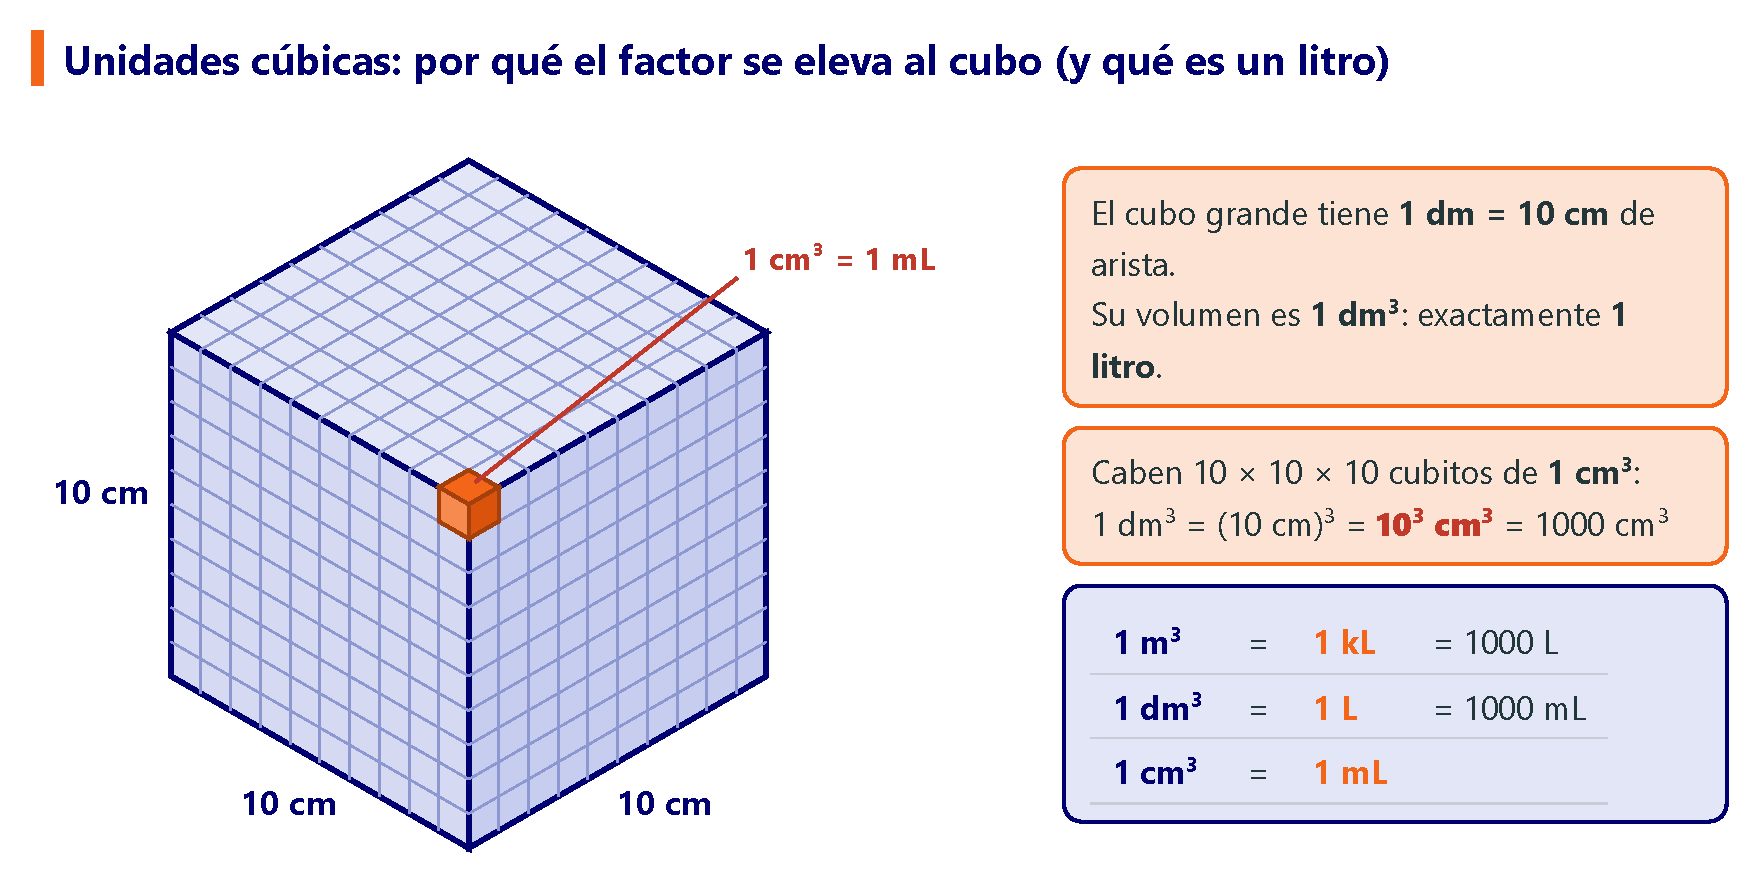
\includegraphics[width=0.9\textwidth]{FigurasSVG/Unit_1_Matter_Measurement/pdf/cube_units_es.pdf}
    \caption{Un decímetro cúbico (un litro) contiene \(10^{3}\) centímetros cúbicos (mililitros).}
    \label{fig:u1_cube_units}
\end{figure}

\begin{impt}
    \negsubro{Truco para el volumen}: hacemos lo mismo que con la superficie, pero ahora \textbf{elevamos el factor de la longitud al cubo}.
    \begin{equation*}
        \text{Longitud: } \dfrac{\qty{e2}{\cm}}{\qty{1}{\m}}
        \quad\Longrightarrow\quad
        \text{Volumen: } \left(\dfrac{\qty{e2}{\cm}}{\qty{1}{\m}}\right)^{3} = \dfrac{\qty{e6}{\cubic\cm}}{\qty{1}{\cubic\m}}
    \end{equation*}
    Por tanto, cada escalón de la escalera de unidades de volumen vale \(10^{3} = 1000\).
\end{impt}

\begin{example}
    \textbf{Expresa \qty{0.5}{\cubic\metre} en \unit{\cubic\mm}.} \\
    Cambio simple: \(\qty{1}{\m} = \qty{e3}{\mm}\). Elevando el factor al cubo:
    \begin{equation*}
        \num{0.5}\,\cancelunit{\cubic\m} \cdot \left(\dfrac{\qty{e3}{\mm}}{1\,\cancelunit{\m}}\right)^{3}
        = \num{0.5}\,\cancelunit{\cubic\m} \cdot \dfrac{\qty{e9}{\cubic\mm}}{1\,\cancelunit{\cubic\m}}
        = \textcolor{red}{\qty{5e8}{\cubic\mm}}
    \end{equation*}
\end{example}

\begin{example}
    \textbf{Expresa \qty{850}{\cubic\deca\metre} en \unit{\cubic\km}.} \\
    Cambio simple: \(\qty{1}{\km} = \qty{e2}{\deca\m}\). Elevando el factor al cubo:
    \begin{equation*}
        \num{850}\,\cancelunit{\cubic\deca\m} \cdot \left(\dfrac{\qty{1}{\km}}{\num{e2}\,\cancelunit{\deca\m}}\right)^{3}
        = \num{850}\,\cancelunit{\cubic\deca\m} \cdot \dfrac{\qty{1}{\cubic\km}}{\num{e6}\,\cancelunit{\cubic\deca\m}}
        = \qty{850e-6}{\cubic\km} = \textcolor{red}{\qty{8.5e-4}{\cubic\km}}
    \end{equation*}
\end{example}

\begin{exercise}
    Cambia de unidades estas cantidades usando factores de conversión:
    \begin{enumerate}[label=\letraminuscula]
        \item \(\qty{73.357}{\cubic\cm} \to \unit{\cubic\mm}\)
        \item \(\qty{1.0576}{\cubic\deca\metre} \to \unit{\cubic\dm}\)
        \item \(\qty{2500}{\cubic\cm} \to \unit{\cubic\m}\)
    \end{enumerate}
    \begin{solu}
        \begin{enumerate}[label=\alph*)]
            \item \(\num{73.357}\,\unit{\cubic\cm} \cdot \left(\dfrac{\qty{e1}{\mm}}{\qty{1}{\cm}}\right)^{3} = \num{73.357}\,\unit{\cubic\cm} \cdot \dfrac{\qty{e3}{\cubic\mm}}{\qty{1}{\cubic\cm}} = \qty{73357}{\cubic\mm}\)
            \item \(\num{1.0576}\,\unit{\cubic\deca\m} \cdot \left(\dfrac{\qty{e2}{\dm}}{\qty{1}{\deca\m}}\right)^{3} = \num{1.0576}\,\unit{\cubic\deca\m} \cdot \dfrac{\qty{e6}{\cubic\dm}}{\qty{1}{\cubic\deca\m}} = \qty{1.0576e6}{\cubic\dm}\)
            \item \(\num{2500}\,\unit{\cubic\cm} \cdot \left(\dfrac{\qty{1}{\m}}{\qty{e2}{\cm}}\right)^{3} = \num{2500}\,\unit{\cubic\cm} \cdot \dfrac{\qty{1}{\cubic\m}}{\qty{e6}{\cubic\cm}} = \qty{2.5e-3}{\cubic\m}\)
        \end{enumerate}
    \end{solu}
\end{exercise}

\begin{exercise}
    Cambia de unidades estas cantidades usando factores de conversión:
    \begin{enumerate}[label=\letraminuscula]
        \item \(\qty{40}{\cubic\cm} \to \unit{\cubic\dm}\)
        \item \(\qty{e3}{\cubic\km} \to \unit{\cubic\hecto\m}\)
        \item \(\qty{3}{\cubic\deca\m} \to \unit{\cubic\cm}\)
        \item \(\qty{e2}{\cubic\cm} \to \unit{\cubic\dm}\)
        \item \(\qty{7}{\cubic\mm} \to \unit{\cubic\deca\m}\)
        \item \(\qty{2e-2}{\cubic\m} \to \unit{\cubic\mm}\)
        \item \(\qty{5e2}{\cubic\km} \to \unit{\cubic\hecto\m}\)
        \item \(\qty{4.23}{\cubic\deca\m} \to \unit{\cubic\cm}\)
        \item \(\qty{48}{\cubic\cm} \to \unit{\cubic\dm}\)
    \end{enumerate}
    \begin{solu}
        \begin{enumerate}[label=\alph*)]
            \item \(\num{40}\,\unit{\cubic\cm} \cdot \left(\dfrac{\qty{1}{\dm}}{\qty{e1}{\cm}}\right)^{3} = \num{40}\,\unit{\cubic\cm} \cdot \dfrac{\qty{1}{\cubic\dm}}{\qty{e3}{\cubic\cm}} = \qty{4e-2}{\cubic\dm} = \qty{0.04}{\cubic\dm}\)
            \item \(\num{e3}\,\unit{\cubic\km} \cdot \left(\dfrac{\qty{e1}{\hecto\m}}{\qty{1}{\km}}\right)^{3} = \num{e3}\,\unit{\cubic\km} \cdot \dfrac{\qty{e3}{\cubic\hecto\m}}{\qty{1}{\cubic\km}} = \qty{e6}{\cubic\hecto\m}\)
            \item \(\num{3}\,\unit{\cubic\deca\m} \cdot \left(\dfrac{\qty{e3}{\cm}}{\qty{1}{\deca\m}}\right)^{3} = \num{3}\,\unit{\cubic\deca\m} \cdot \dfrac{\qty{e9}{\cubic\cm}}{\qty{1}{\cubic\deca\m}} = \qty{3e9}{\cubic\cm}\)
            \item \(\num{e2}\,\unit{\cubic\cm} \cdot \left(\dfrac{\qty{1}{\dm}}{\qty{e1}{\cm}}\right)^{3} = \num{e2}\,\unit{\cubic\cm} \cdot \dfrac{\qty{1}{\cubic\dm}}{\qty{e3}{\cubic\cm}} = \qty{e-1}{\cubic\dm} = \qty{0.1}{\cubic\dm}\)
            \item \(\num{7}\,\unit{\cubic\mm} \cdot \left(\dfrac{\qty{1}{\deca\m}}{\qty{e4}{\mm}}\right)^{3} = \num{7}\,\unit{\cubic\mm} \cdot \dfrac{\qty{1}{\cubic\deca\m}}{\qty{e12}{\cubic\mm}} = \qty{7e-12}{\cubic\deca\m}\)
            \item \(\num{2e-2}\,\unit{\cubic\m} \cdot \left(\dfrac{\qty{e3}{\mm}}{\qty{1}{\m}}\right)^{3} = \num{2e-2}\,\unit{\cubic\m} \cdot \dfrac{\qty{e9}{\cubic\mm}}{\qty{1}{\cubic\m}} = \qty{2e7}{\cubic\mm}\)
            \item \(\num{5e2}\,\unit{\cubic\km} \cdot \left(\dfrac{\qty{e1}{\hecto\m}}{\qty{1}{\km}}\right)^{3} = \num{5e2}\,\unit{\cubic\km} \cdot \dfrac{\qty{e3}{\cubic\hecto\m}}{\qty{1}{\cubic\km}} = \qty{5e5}{\cubic\hecto\m}\)
            \item \(\num{4.23}\,\unit{\cubic\deca\m} \cdot \left(\dfrac{\qty{e3}{\cm}}{\qty{1}{\deca\m}}\right)^{3} = \num{4.23}\,\unit{\cubic\deca\m} \cdot \dfrac{\qty{e9}{\cubic\cm}}{\qty{1}{\cubic\deca\m}} = \qty{4.23e9}{\cubic\cm}\)
            \item \(\num{48}\,\unit{\cubic\cm} \cdot \left(\dfrac{\qty{1}{\dm}}{\qty{e1}{\cm}}\right)^{3} = \num{48}\,\unit{\cubic\cm} \cdot \dfrac{\qty{1}{\cubic\dm}}{\qty{e3}{\cubic\cm}} = \qty{4.8e-2}{\cubic\dm} = \qty{0.048}{\cubic\dm}\)
        \end{enumerate}
    \end{solu}
\end{exercise}

%------------------------------------------------

\subsubsection{Volumen y capacidad: unidades cúbicas y litros}

Hablamos de \textbf{volumen} para el espacio que ocupa un cuerpo y de \textbf{capacidad} para lo que cabe en un recipiente, pero son la misma magnitud, así que sus unidades están relacionadas. Las tres equivalencias clave son:

\begin{table}[H]
    \centering
    \renewcommand{\arraystretch}{1.4}
    \begin{tabular}{ccc}
        \toprule
        \textbf{Volumen} & & \textbf{Capacidad} \\
        \midrule
        \qty{1}{\cubic\m} & = & \qty{1}{\kilo\litre} \\
        \qty{1}{\cubic\dm} & = & \qty{1}{\litre} \\
        \qty{1}{\cubic\cm} & = & \qty{1}{\mL} \\
        \bottomrule
    \end{tabular}
    \caption{Equivalencias entre unidades de volumen y de capacidad.}
    \label{tab:u1_volume_capacity}
\end{table}

\begin{impt}
    Para cambiar entre unidades cúbicas y litros:
    \begin{enumerate}[label=\numberballmDarkTeal]
        \item Usa los factores de conversión de volumen (al cubo) o de capacidad (simples) hasta llegar a una de las tres unidades «pareja»: \unit{\cubic\m}--\unit{\kilo\litre}, \unit{\cubic\dm}--\unit{\litre} o \unit{\cubic\cm}--\unit{\mL}.
        \item Salta de volumen a capacidad (o al revés) con un factor como \(\dfrac{\qty{1}{\litre}}{\qty{1}{\cubic\dm}}\), que vale 1.
    \end{enumerate}
\end{impt}

\begin{example}
    \textbf{Expresa \qty{2.5}{\cubic\m} en litros.}
    \begin{equation*}
        \num{2.5}\,\cancelunit{\cubic\m} \cdot \dfrac{\qty{1}{\kilo\litre}}{1\,\cancelunit{\cubic\m}} \cdot \dfrac{\qty{e3}{\litre}}{1\,\cancelunit{\kilo\litre}} = \textcolor{red}{\qty{2.5e3}{\litre}} = \qty{2500}{\litre}
    \end{equation*}
\end{example}

\begin{example}
    \textbf{Una lata de refresco contiene \qty{33}{\centi\litre}. Exprésalo en \unit{\cubic\cm}.}
    \begin{equation*}
        \num{33}\,\cancelunit{\centi\litre} \cdot \dfrac{\num{e1}\,\cancelunit{\mL}}{1\,\cancelunit{\centi\litre}} \cdot \dfrac{\qty{1}{\cubic\cm}}{1\,\cancelunit{\mL}} = \textcolor{red}{\qty{330}{\cubic\cm}}
    \end{equation*}
\end{example}

\begin{example}
    \textbf{Expresa \qty{750}{\mL} en \unit{\cubic\m}.}
    \begin{equation*}
        \num{750}\,\cancelunit{\mL} \cdot \dfrac{1\,\cancelunit{\cubic\cm}}{1\,\cancelunit{\mL}} \cdot \left(\dfrac{\qty{1}{\m}}{\num{e2}\,\cancelunit{\cm}}\right)^{3}
        = \num{750}\,\cancelunit{\cubic\cm} \cdot \dfrac{\qty{1}{\cubic\m}}{\num{e6}\,\cancelunit{\cubic\cm}} = \textcolor{red}{\qty{7.5e-4}{\cubic\m}}
    \end{equation*}
\end{example}

\begin{exercise}
    Una piscina olímpica contiene 2,5 millones de litros de agua (\qty{2.5e6}{\litre}). Exprésalo en \unit{\cubic\metre}.
    \begin{solu}
        \(\num{2.5e6}\,\unit{\litre} \cdot \dfrac{\qty{1}{\cubic\dm}}{\qty{1}{\litre}} \cdot \left(\dfrac{\qty{1}{\m}}{\qty{e1}{\dm}}\right)^{3} = \num{2.5e6}\,\unit{\cubic\dm} \cdot \dfrac{\qty{1}{\cubic\m}}{\qty{e3}{\cubic\dm}} = \qty{2.5e3}{\cubic\m} = \qty{2500}{\cubic\m}\).
    \end{solu}
\end{exercise}

\begin{exercise}
    Cambia de unidades: \textbf{a)} \qty{1.5}{\litre} \(\to\) \unit{\cubic\cm}; \textbf{b)} \qty{40}{\cubic\cm} \(\to\) \unit{\centi\litre}; \textbf{c)} \qty{0.2}{\cubic\m} \(\to\) \unit{\litre}; \textbf{d)} \qty{5}{\mL} \(\to\) \unit{\cubic\dm}.
    \begin{solu}
        a) \(\num{1.5}\,\unit{\litre} \cdot \dfrac{\qty{e3}{\mL}}{\qty{1}{\litre}} \cdot \dfrac{\qty{1}{\cubic\cm}}{\qty{1}{\mL}} = \qty{1500}{\cubic\cm}\) \\
        b) \(\num{40}\,\unit{\cubic\cm} \cdot \dfrac{\qty{1}{\mL}}{\qty{1}{\cubic\cm}} \cdot \dfrac{\qty{1}{\centi\litre}}{\qty{e1}{\mL}} = \qty{4}{\centi\litre}\) \\
        c) \(\num{0.2}\,\unit{\cubic\m} \cdot \dfrac{\qty{1}{\kilo\litre}}{\qty{1}{\cubic\m}} \cdot \dfrac{\qty{e3}{\litre}}{\qty{1}{\kilo\litre}} = \qty{200}{\litre}\) \\
        d) \(\num{5}\,\unit{\mL} \cdot \dfrac{\qty{1}{\litre}}{\qty{e3}{\mL}} \cdot \dfrac{\qty{1}{\cubic\dm}}{\qty{1}{\litre}} = \qty{5e-3}{\cubic\dm}\)
    \end{solu}
\end{exercise}

\begin{exercise}
    Una pecera es un prisma rectangular de \qty{50}{\cm} de largo, \qty{30}{\cm} de ancho y \qty{40}{\cm} de alto.
    \begin{enumerate}[label=\letraminuscula]
        \item Calcula su volumen en \unit{\cubic\cm}.
        \item ¿Cuántos litros de agua hacen falta para llenarla por completo?
    \end{enumerate}
    \begin{solu}
        \begin{enumerate}[label=\alph*)]
            \item \(V = \qty{50}{\cm} \cdot \qty{30}{\cm} \cdot \qty{40}{\cm} = \qty{60000}{\cubic\cm} = \qty{6e4}{\cubic\cm}\).
            \item \(\num{6e4}\,\unit{\cubic\cm} \cdot \dfrac{\qty{1}{\mL}}{\qty{1}{\cubic\cm}} \cdot \dfrac{\qty{1}{\litre}}{\qty{e3}{\mL}} = \qty{60}{\litre}\).
        \end{enumerate}
    \end{solu}
\end{exercise}

\begin{exercise}
    Cambia de unidades estas cantidades usando factores de conversión:
    \begin{enumerate}[label=\letraminuscula]
        \item \(\qty{0.02}{\cubic\deca\m} \to \unit{\mL}\)
        \item \(\qty{100}{\mL} \to \unit{\cubic\m}\)
        \item \(\qty{300}{\litre} \to \unit{\cubic\deca\m}\)
    \end{enumerate}
    \begin{solu}
        \begin{enumerate}[label=\alph*)]
            \item \(\num{0.02}\,\unit{\cubic\deca\m} \cdot \left(\dfrac{\qty{e3}{\cm}}{\qty{1}{\deca\m}}\right)^{3} \cdot \dfrac{\qty{1}{\mL}}{\qty{1}{\cubic\cm}} = \num{0.02}\,\unit{\cubic\deca\m} \cdot \dfrac{\qty{e9}{\cubic\cm}}{\qty{1}{\cubic\deca\m}} \cdot \dfrac{\qty{1}{\mL}}{\qty{1}{\cubic\cm}} = \qty{2e7}{\mL}\)
            \item \(\num{100}\,\unit{\mL} \cdot \dfrac{\qty{1}{\cubic\cm}}{\qty{1}{\mL}} \cdot \left(\dfrac{\qty{1}{\m}}{\qty{e2}{\cm}}\right)^{3} = \num{100}\,\unit{\cubic\cm} \cdot \dfrac{\qty{1}{\cubic\m}}{\qty{e6}{\cubic\cm}} = \qty{e-4}{\cubic\m}\)
            \item \(\num{300}\,\unit{\litre} \cdot \dfrac{\qty{1}{\cubic\dm}}{\qty{1}{\litre}} \cdot \left(\dfrac{\qty{1}{\deca\m}}{\qty{e2}{\dm}}\right)^{3} = \num{300}\,\unit{\cubic\dm} \cdot \dfrac{\qty{1}{\cubic\deca\m}}{\qty{e6}{\cubic\dm}} = \qty{3e-4}{\cubic\deca\m}\)
        \end{enumerate}
    \end{solu}
\end{exercise}

%------------------------------------------------

\subsubsection{El tiempo}

En el SI, el tiempo se mide en \textbf{segundos} (\unit{\s}). Para tiempos más largos usamos minutos, horas, días, semanas y años. \textbf{Cuidado}: estas unidades \textbf{no} están relacionadas por potencias de 10, así que no podemos usar la escalera de los prefijos. Hay que usar sus equivalencias reales.

\begin{figure}[H]
    \centering
    % [FIGURA ORIGINAL] \includegraphics[width=\textwidth]{Unit_1/time_chain}
    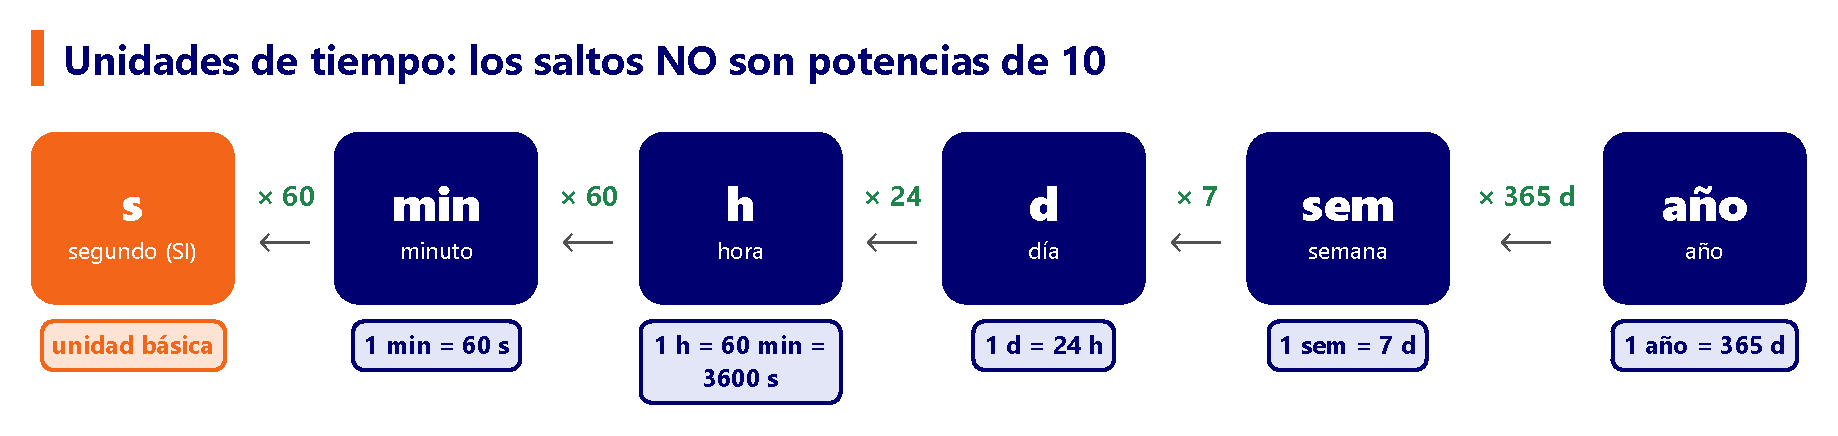
\includegraphics[width=\textwidth]{FigurasSVG/Unit_1_Matter_Measurement/pdf/time_chain_es.pdf}
    \caption{La cadena de las unidades de tiempo.}
    \label{fig:u1_time_chain}
\end{figure}

\begin{table}[H]
    \centering
    \renewcommand{\arraystretch}{2.4}
    \begin{tabular}{ll}
        \toprule
        \textbf{Equivalencia} & \textbf{Factores de conversión} \\
        \midrule
        \(\qty{1}{\minute} = \qty{60}{\s}\) & \(\dfrac{\qty{60}{\s}}{\qty{1}{\minute}}\) o \(\dfrac{\qty{1}{\minute}}{\qty{60}{\s}}\) \\
        \(\qty{1}{\hour} = \qty{60}{\minute} = \qty{3600}{\s}\) & \(\dfrac{\qty{3600}{\s}}{\qty{1}{\hour}}\) o \(\dfrac{\qty{1}{\hour}}{\qty{3600}{\s}}\) \\
        \(\qty{1}{\day} = \qty{24}{\hour}\) & \(\dfrac{\qty{24}{\hour}}{\qty{1}{\day}}\) o \(\dfrac{\qty{1}{\day}}{\qty{24}{\hour}}\) \\
        \(\qty{1}{\text{semana}} = \qty{7}{\day}\) & \(\dfrac{\qty{7}{\day}}{\qty{1}{\text{semana}}}\) o \(\dfrac{\qty{1}{\text{semana}}}{\qty{7}{\day}}\) \\
        \(\qty{1}{	ext{\text{año}}} = \qty{365}{\day}\) & \(\dfrac{\qty{365}{\day}}{\qty{1}{	ext{\text{año}}}}\) o \(\dfrac{\qty{1}{	ext{\text{año}}}}{\qty{365}{\day}}\) \\
        \bottomrule
    \end{tabular}
    \caption{Equivalencias de tiempo y sus factores de conversión.}
    \label{tab:u1_time}
\end{table}

\begin{example}
    \textbf{Expresa \qty{5000}{\s} en horas.}
    \begin{equation*}
        \num{5000}\,\cancelunit{\s} \cdot \dfrac{\qty{1}{\hour}}{\num{3600}\,\cancelunit{\s}} = \dfrac{5000}{3600}\,\unit{\hour} = \textcolor{red}{\qty{1.39}{\hour}}
    \end{equation*}
\end{example}

\begin{example}
    \textbf{¿Cuántos segundos hay en 2 semanas?} No hay una equivalencia directa, así que encadenamos varios factores:
    \begin{equation*}
        \num{2}\,\cancelunit{\text{semanas}} \cdot \dfrac{\num{7}\,\cancelunit{\day}}{1\,\cancelunit{\text{semana}}} \cdot \dfrac{\num{24}\,\cancelunit{\hour}}{1\,\cancelunit{\day}} \cdot \dfrac{\qty{3600}{\s}}{1\,\cancelunit{\hour}} = \qty{1209600}{\s} \approx \textcolor{red}{\qty{1.21e6}{\s}}
    \end{equation*}
\end{example}

\begin{exercise}
    Una película dura \qty{135}{\minute}. ¿Cuántas horas dura? Una canción dura \qty{4.5}{\minute}. ¿Cuántos segundos dura?
    \begin{solu}
        \(\num{135}\,\unit{\minute} \cdot \dfrac{\qty{1}{\hour}}{\qty{60}{\minute}} = \qty{2.25}{\hour}\). \\
        \(\num{4.5}\,\unit{\minute} \cdot \dfrac{\qty{60}{\s}}{\qty{1}{\minute}} = \qty{270}{\s}\).
    \end{solu}
\end{exercise}

\begin{exercise}
    Cambia de unidades: \textbf{a)} \qty{3}{\day} \(\to\) \unit{\minute}; \textbf{b)} \qty{90}{\minute} \(\to\) \unit{\hour}; \textbf{c)} \qty{86400}{\s} \(\to\) \unit{\day}; \textbf{d)} \qty{1}{	ext{\text{año}}} \(\to\) semanas.
    \begin{solu}
        a) \(\num{3}\,\unit{\day} \cdot \dfrac{\qty{24}{\hour}}{\qty{1}{\day}} \cdot \dfrac{\qty{60}{\minute}}{\qty{1}{\hour}} = \qty{4320}{\minute}\) \\
        b) \(\num{90}\,\unit{\minute} \cdot \dfrac{\qty{1}{\hour}}{\qty{60}{\minute}} = \qty{1.5}{\hour}\) \\
        c) \(\num{86400}\,\unit{\s} \cdot \dfrac{\qty{1}{\hour}}{\qty{3600}{\s}} \cdot \dfrac{\qty{1}{\day}}{\qty{24}{\hour}} = \qty{1}{\day}\) \\
        d) \(\num{1}\,\unit{	ext{\text{año}}} \cdot \dfrac{\qty{365}{\day}}{\qty{1}{	ext{\text{año}}}} \cdot \dfrac{\qty{1}{\text{semana}}}{\qty{7}{\day}} \approx \qty{52.1}{\text{semanas}}\)
    \end{solu}
\end{exercise}

\begin{exercise}
    Tienes 12 años. ¿Cuántos segundos has vivido, aproximadamente? Da el resultado como potencia de 10.
    \begin{solu}
        \(\num{12}\,\unit{	ext{\text{años}}} \cdot \dfrac{\qty{365}{\day}}{\qty{1}{	ext{\text{año}}}} \cdot \dfrac{\qty{24}{\hour}}{\qty{1}{\day}} \cdot \dfrac{\qty{3600}{\s}}{\qty{1}{\hour}} = \qty{378432000}{\s} \approx \qty{3.78e8}{\s}\).
    \end{solu}
\end{exercise}

\begin{exercise}
    Cambia de unidades estos tiempos usando factores de conversión:
    \begin{enumerate}[label=\letraminuscula]
        \item \(\qty{340}{\minute} \to \unit{\s}\)
        \item \(\qty{6.2}{\hour} \to \unit{\minute}\)
        \item \(\qty{10}{\hour} \to \unit{\s}\)
        \item \(\qty{28}{\text{semanas}} \to \unit{\minute}\)
        \item \(\qty{22}{\text{semanas}} \to \unit{\hour}\)
    \end{enumerate}
    \begin{solu}
        \begin{enumerate}[label=\alph*)]
            \item \(\num{340}\,\unit{\minute} \cdot \dfrac{\qty{60}{\s}}{\qty{1}{\minute}} = \qty{20400}{\s} \approx \qty{2.04e4}{\s}\)
            \item \(\num{6.2}\,\unit{\hour} \cdot \dfrac{\qty{60}{\minute}}{\qty{1}{\hour}} = \qty{372}{\minute}\)
            \item \(\num{10}\,\unit{\hour} \cdot \dfrac{\qty{3600}{\s}}{\qty{1}{\hour}} = \qty{36000}{\s} = \qty{3.6e4}{\s}\)
            \item \(\num{28}\,\unit{\text{semanas}} \cdot \dfrac{\qty{7}{\day}}{\qty{1}{\text{semana}}} \cdot \dfrac{\qty{24}{\hour}}{\qty{1}{\day}} \cdot \dfrac{\qty{60}{\minute}}{\qty{1}{\hour}} = \qty{282240}{\minute} \approx \qty{2.82e5}{\minute}\)
            \item \(\num{22}\,\unit{\text{semanas}} \cdot \dfrac{\qty{7}{\day}}{\qty{1}{\text{semana}}} \cdot \dfrac{\qty{24}{\hour}}{\qty{1}{\day}} = \qty{3696}{\hour}\)
        \end{enumerate}
    \end{solu}
\end{exercise}

%------------------------------------------------

\subsubsection{La velocidad}

La velocidad es una magnitud derivada (longitud \(\div\) tiempo), así que su unidad tiene \textbf{dos} partes. Para cambiarla usamos \textbf{dos} factores de conversión: uno para la longitud (numerador) y otro para el tiempo (denominador).

\begin{impt}
    \negsubro{Unidades con más de una magnitud: una unidad cada vez, en orden}

    Cuando una unidad está formada por dos magnitudes (\unit{\km\per\hour}, \unit{\g\per\mL}\ldots), \textbf{no} intentamos cambiar las dos a la vez. Vamos \textbf{en orden}:
    \begin{enumerate}[label=\numberballmDarkTeal]
        \item Primero cambiamos \textbf{una} de las unidades (por ejemplo, la longitud: \unit{\km} \(\to\) \unit{\m}) con su propio factor de conversión.
        \item Después cambiamos la \textbf{otra} unidad (el tiempo: \unit{\hour} \(\to\) \unit{\s}) con un segundo factor de conversión.
        \item Por último simplificamos las unidades y calculamos.
        \item Los pasos 1 y 2 \textbf{se pueden y se deben} hacer \textbf{todo seguido, en una sola línea}: escribimos el primer factor de conversión y, justo detrás, el segundo, sin pararnos a calcular el resultado intermedio. Simplificamos todas las unidades al final y hacemos una sola operación.
    \end{enumerate}
    Paso a paso para \qty{90}{\km\per\hour}:
    \begin{equation*}
        \underbrace{\num{90}\,\dfrac{\cancelunit{\km}}{\unit{\hour}} \cdot \dfrac{\qty{e3}{\m}}{1\,\cancelunit{\km}} = \qty{90000}{\m\per\hour}}_{\text{1.º: la longitud}}
        \quad\Longrightarrow\quad
        \underbrace{\num{90000}\,\dfrac{\unit{\m}}{\cancelunit{\hour}} \cdot \dfrac{1\,\cancelunit{\hour}}{\qty{3600}{\s}} = \qty{25}{\m\per\s}}_{\text{2.º: el tiempo}}
    \end{equation*}
    Todo seguido, en una sola línea (así es como debemos hacerlo):
    \begin{equation*}
        \num{90}\,\dfrac{\cancelunit{\km}}{\cancelunit{\hour}} \cdot \underbrace{\dfrac{\qty{e3}{\m}}{1\,\cancelunit{\km}}}_{\text{1.º: longitud}} \cdot \underbrace{\dfrac{1\,\cancelunit{\hour}}{\qty{3600}{\s}}}_{\text{2.º: tiempo}} = \dfrac{\num{90e3}}{3600}\,\unit{\m\per\s} = \qty{25}{\m\per\s}
    \end{equation*}
\end{impt}

\begin{figure}[H]
    \centering
    % [FIGURA ORIGINAL] \includegraphics[width=0.85\textwidth]{Unit_1/speed_shortcut}
    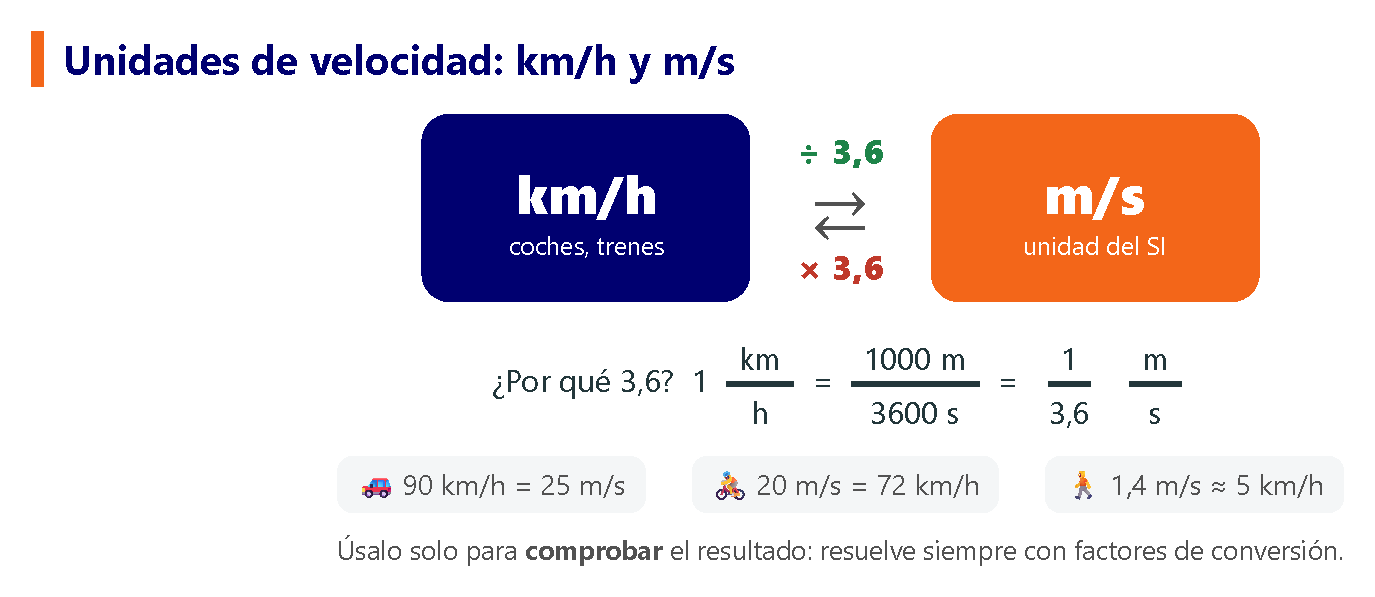
\includegraphics[width=0.85\textwidth]{FigurasSVG/Unit_1_Matter_Measurement/pdf/speed_shortcut_es.pdf}
    \caption{Las dos unidades de velocidad más habituales y una forma rápida de comprobar el resultado.}
    \label{fig:u1_speed_shortcut}
\end{figure}

\begin{example}
    \textbf{Un coche circula a \qty{90}{\km\per\hour}. Expresa esta velocidad en \unit{\m\per\s}.}
    \begin{equation*}
        \num{90}\,\dfrac{\cancelunit{\km}}{\cancelunit{\hour}} \cdot \dfrac{\qty{e3}{\m}}{1\,\cancelunit{\km}} \cdot \dfrac{1\,\cancelunit{\hour}}{\qty{3600}{\s}} = \dfrac{\num{90e3}}{3600}\,\unit{\m\per\s} = \textcolor{red}{\qty{25}{\m\per\s}}
    \end{equation*}
\end{example}

\begin{example}
    \textbf{Un ciclista va a \qty{20}{\m\per\s}. Expresa esta velocidad en \unit{\km\per\hour}.}
    \begin{equation*}
        \num{20}\,\dfrac{\cancelunit{\m}}{\cancelunit{\s}} \cdot \dfrac{\qty{1}{\km}}{\num{e3}\,\cancelunit{\m}} \cdot \dfrac{\num{3600}\,\cancelunit{\s}}{\qty{1}{\hour}} = \textcolor{red}{\qty{72}{\km\per\hour}}
    \end{equation*}
\end{example}

\begin{marker}
    \textbf{Dividir o multiplicar por 3,6 es solo una ayuda.} El «truco» de la figura (\(\div\,3.6\) para pasar de \unit{\km\per\hour} a \unit{\m\per\s}, y \(\times\,3.6\) para volver) solo sirve para \textbf{comprobar} el resultado, y \textbf{solo funciona para ese cambio}: \unit{\km\per\hour} \(\leftrightarrow\) \unit{\m\per\s}. Para cualquier otra unidad de velocidad (\unit{\cm\per\s}, \unit{\m\per\minute}, \unit{\km\per\minute}\ldots) da un resultado erróneo. La forma correcta, que funciona \textbf{siempre}, es usar \textbf{factores de conversión}.
\end{marker}

\begin{example}
    \textbf{Una tortuga camina a \qty{12}{\m\per\minute}. Expresa esta velocidad en \unit{\m\per\s}.} Solo cambia el tiempo, así que basta con un factor:
    \begin{equation*}
        \num{12}\,\dfrac{\unit{\m}}{\cancelunit{\minute}} \cdot \dfrac{1\,\cancelunit{\minute}}{\qty{60}{\s}} = \textcolor{red}{\qty{0.2}{\m\per\s}}
    \end{equation*}
\end{example}

\begin{example}
    \textbf{Un coche de juguete se mueve a \qty{45}{\cm\per\s}. Expresa esta velocidad en \unit{\km\per\hour}.} Primero la longitud y después el tiempo:
    \begin{equation*}
        \num{45}\,\dfrac{\cancelunit{\cm}}{\cancelunit{\s}} \cdot \dfrac{\qty{1}{\km}}{\num{e5}\,\cancelunit{\cm}} \cdot \dfrac{\num{3600}\,\cancelunit{\s}}{\qty{1}{\hour}} = \dfrac{\num{45} \cdot \num{3600}}{\num{e5}}\,\unit{\km\per\hour} = \textcolor{red}{\qty{1.62}{\km\per\hour}}
    \end{equation*}
\end{example}

\begin{example}
    \textbf{Un avión vuela a \qty{15}{\km\per\minute}. Expresa esta velocidad en \unit{\m\per\s}.} Primero la longitud y después el tiempo:
    \begin{equation*}
        \num{15}\,\dfrac{\cancelunit{\km}}{\cancelunit{\minute}} \cdot \dfrac{\qty{e3}{\m}}{1\,\cancelunit{\km}} \cdot \dfrac{1\,\cancelunit{\minute}}{\qty{60}{\s}} = \dfrac{\num{15e3}}{60}\,\unit{\m\per\s} = \textcolor{red}{\qty{250}{\m\per\s}}
    \end{equation*}
\end{example}

\begin{example}
    \textbf{Un caracol avanza a \qty{0.5}{\mm\per\s}. Expresa esta velocidad en \unit{\m\per\hour}.} Primero la longitud y después el tiempo:
    \begin{equation*}
        \num{0.5}\,\dfrac{\cancelunit{\mm}}{\cancelunit{\s}} \cdot \dfrac{\qty{1}{\m}}{\num{e3}\,\cancelunit{\mm}} \cdot \dfrac{\num{3600}\,\cancelunit{\s}}{\qty{1}{\hour}} = \textcolor{red}{\qty{1.8}{\m\per\hour}}
    \end{equation*}
\end{example}

\begin{exercise}
    Una atleta corre \qty{100}{\metre} en \qty{11.5}{\s}. Calcula su velocidad media en \unit{\m\per\s} y en \unit{\km\per\hour}.
    \begin{solu}
        \(v = \dfrac{\qty{100}{\m}}{\qty{11.5}{\s}} \approx \qty{8.70}{\m\per\s}\). \\
        \(\num{8.70}\,\dfrac{\unit{\m}}{\unit{\s}} \cdot \dfrac{\qty{1}{\km}}{\qty{e3}{\m}} \cdot \dfrac{\qty{3600}{\s}}{\qty{1}{\hour}} \approx \qty{31.3}{\km\per\hour}\).
    \end{solu}
\end{exercise}

\begin{exercise}
    Cambia de unidades estas velocidades:
    \begin{enumerate}[label=\letraminuscula]
        \item El límite de velocidad en autovía, \qty{120}{\km\per\hour}, a \unit{\m\per\s}.
        \item La velocidad de la luz, \qty{3e5}{\km\per\s}, a \unit{\m\per\s}.
        \item Un caracol que avanza a \qty{1.3}{\cm\per\s}, a \unit{\km\per\hour}.
    \end{enumerate}
    \begin{solu}
        \begin{enumerate}[label=\alph*)]
            \item \(\num{120}\,\dfrac{\unit{\km}}{\unit{\hour}} \cdot \dfrac{\qty{e3}{\m}}{\qty{1}{\km}} \cdot \dfrac{\qty{1}{\hour}}{\qty{3600}{\s}} \approx \qty{33.3}{\m\per\s}\)
            \item \(\num{3e5}\,\dfrac{\unit{\km}}{\unit{\s}} \cdot \dfrac{\qty{e3}{\m}}{\qty{1}{\km}} = \qty{3e8}{\m\per\s}\)
            \item \(\num{1.3}\,\dfrac{\unit{\cm}}{\unit{\s}} \cdot \dfrac{\qty{1}{\km}}{\qty{e5}{\cm}} \cdot \dfrac{\qty{3600}{\s}}{\qty{1}{\hour}} \approx \qty{0.047}{\km\per\hour}\)
        \end{enumerate}
    \end{solu}
\end{exercise}

\begin{exercise}
    Cambia de unidades: \textbf{a)} \qty{36}{\m\per\s} \(\to\) \unit{\km\per\hour}; \textbf{b)} \qty{100}{\km\per\hour} \(\to\) \unit{\m\per\s}.
    \begin{solu}
        a) \(\num{36}\,\dfrac{\unit{\m}}{\unit{\s}} \cdot \dfrac{\qty{1}{\km}}{\qty{e3}{\m}} \cdot \dfrac{\qty{3600}{\s}}{\qty{1}{\hour}} = \qty{129.6}{\km\per\hour}\) \\
        b) \(\num{100}\,\dfrac{\unit{\km}}{\unit{\hour}} \cdot \dfrac{\qty{e3}{\m}}{\qty{1}{\km}} \cdot \dfrac{\qty{1}{\hour}}{\qty{3600}{\s}} \approx \qty{27.8}{\m\per\s}\)
    \end{solu}
\end{exercise}

%------------------------------------------------

\subsubsection{La densidad}

La densidad también combina dos magnitudes (masa y volumen), así que normalmente necesitamos \textbf{dos} factores de conversión, uno para cada unidad. Recuerda ir \textbf{en orden}: primero cambiamos la unidad de masa y después la de volumen, siempre \textbf{una cada vez}.

\begin{example}
    \textbf{Expresa la densidad del kétchup, \qty{1.16}{\g\per\mL}, en \unit{\kg\per\cubic\metre}.}
    \begin{enumerate}[label=\numberballmDarkTeal]
        \item Equivalencias: \(\qty{1}{\kg} = \qty{e3}{\g}\) y \(\qty{1}{\cubic\metre} = \qty{1}{\kilo\litre} = \qty{e6}{\mL}\).
        \item Factores de conversión:
        \(
            \num{1.16}\,\dfrac{\cancelunit{\g}}{\cancelunit{\mL}} \cdot \dfrac{\qty{1}{\kg}}{\num{e3}\,\cancelunit{\g}} \cdot \dfrac{\num{e6}\,\cancelunit{\mL}}{\qty{1}{\cubic\m}}
        \)
        \item Resultado: \(\textcolor{red}{\qty{1.16e3}{\kg\per\cubic\metre}} = \qty{1160}{\kg\per\cubic\m}\).
    \end{enumerate}

\end{example}

\begin{exercise}
    El mercurio es un metal líquido. \qty{1}{\litre} de mercurio tiene una masa de \qty{13.59}{\kg}. Expresa su densidad en \unit{\kg\per\cubic\metre}.
    \begin{solu}
        \(d = \dfrac{\qty{13.59}{\kg}}{\qty{1}{\litre}} \cdot \dfrac{\qty{e3}{\litre}}{\qty{1}{\cubic\m}} = \qty{1.359e4}{\kg\per\cubic\metre}\).
    \end{solu}
\end{exercise}

\begin{exercise}
    El aire que respiramos tiene una densidad de aproximadamente \qty{1.29}{\kg\per\cubic\metre}. Exprésala en \unit{\g\per\litre}.
    \begin{solu}
        \(d = \num{1.29}\,\dfrac{\unit{\kg}}{\unit{\cubic\m}} \cdot \dfrac{\qty{e3}{\g}}{\qty{1}{\kg}} \cdot \dfrac{\qty{1}{\cubic\m}}{\qty{e3}{\litre}} = \qty{1.29}{\g\per\litre}\).
    \end{solu}
\end{exercise}

\begin{exercise}
    Un tipo de madera tiene una densidad de \qty{750}{\kg\per\cubic\metre}. Exprésala en \unit{\g\per\mL} y decide si esta madera flota en el agua.
    \begin{solu}
        \(\num{750}\,\dfrac{\unit{\kg}}{\unit{\cubic\m}} \cdot \dfrac{\qty{e3}{\g}}{\qty{1}{\kg}} \cdot \dfrac{\qty{1}{\cubic\m}}{\qty{e6}{\mL}} = \qty{0.75}{\g\per\mL}\). \\
        Como \(\qty{0.75}{\g\per\mL} < \qty{1.00}{\g\per\mL}\), esta madera \textbf{flota} en el agua.
    \end{solu}
\end{exercise}

\begin{exercise}
    Cambia de unidades estas densidades usando factores de conversión:
    \begin{enumerate}[label=\letraminuscula]
        \item \(\qty{1.05}{\kg\per\cubic\cm} \to \unit{\hecto\gram\per\cubic\mm}\)
        \item \(\qty{0.25}{\g\per\mL} \to \unit{\kg\per\cubic\m}\)
        \item \(\qty{0.05}{\kg\per\cubic\cm} \to \unit{\g\per\mL}\)
    \end{enumerate}
    \begin{solu}
        \begin{enumerate}[label=\alph*)]
            \item \(\num{1.05}\,\dfrac{\unit{\kg}}{\unit{\cubic\cm}} \cdot \dfrac{\qty{e1}{\hecto\gram}}{\qty{1}{\kg}} \cdot \left(\dfrac{\qty{1}{\cm}}{\qty{e1}{\mm}}\right)^{3} = \num{1.05}\,\dfrac{\unit{\kg}}{\unit{\cubic\cm}} \cdot \dfrac{\qty{e1}{\hecto\gram}}{\qty{1}{\kg}} \cdot \dfrac{\qty{1}{\cubic\cm}}{\qty{e3}{\cubic\mm}} = \qty{1.05e-2}{\hecto\gram\per\cubic\mm}\)
            \item \(\num{0.25}\,\dfrac{\unit{\g}}{\unit{\mL}} \cdot \dfrac{\qty{1}{\kg}}{\qty{e3}{\g}} \cdot \dfrac{\qty{e6}{\mL}}{\qty{1}{\cubic\m}} = \qty{250}{\kg\per\cubic\m} = \qty{2.5e2}{\kg\per\cubic\m}\)
            \item \(\num{0.05}\,\dfrac{\unit{\kg}}{\unit{\cubic\cm}} \cdot \dfrac{\qty{e3}{\g}}{\qty{1}{\kg}} \cdot \dfrac{\qty{1}{\cubic\cm}}{\qty{1}{\mL}} = \qty{50}{\g\per\mL}\)
        \end{enumerate}
    \end{solu}
\end{exercise}

\begin{exercise}
    Despeja el volumen, calcúlalo y después pásalo a \unit{\cubic\m}:
    \begin{enumerate}[label=\letraminuscula]
        \item Un lingote de oro tiene una densidad de \qty{19}{\g\per\cubic\cm} y una masa de \qty{9500}{\g}. Calcula el volumen del lingote, en \unit{\cubic\m}.
        \item Una pelota de críquet tiene una densidad de \qty{0.8}{\g\per\cubic\cm} y una masa de \qty{165}{\g}. Calcula el volumen de la pelota, en \unit{\cubic\m}.
    \end{enumerate}
    \begin{solu}
        \begin{enumerate}[label=\alph*)]
            \item \(V = \dfrac{m}{d} = \dfrac{\qty{9500}{\g}}{\qty{19}{\g\per\cubic\cm}} = \qty{500}{\cubic\cm}\). \\
            En \unit{\cubic\m}: \(\num{500}\,\unit{\cubic\cm} \cdot \left(\dfrac{\qty{1}{\m}}{\qty{e2}{\cm}}\right)^{3} = \num{500}\,\unit{\cubic\cm} \cdot \dfrac{\qty{1}{\cubic\m}}{\qty{e6}{\cubic\cm}} = \qty{5e-4}{\cubic\m}\)
            \item \(V = \dfrac{m}{d} = \dfrac{\qty{165}{\g}}{\qty{0.8}{\g\per\cubic\cm}} = \qty{206.25}{\cubic\cm}\). \\
            En \unit{\cubic\m}: \(\num{206.25}\,\unit{\cubic\cm} \cdot \left(\dfrac{\qty{1}{\m}}{\qty{e2}{\cm}}\right)^{3} = \num{206.25}\,\unit{\cubic\cm} \cdot \dfrac{\qty{1}{\cubic\m}}{\qty{e6}{\cubic\cm}} \approx \qty{2.06e-4}{\cubic\m}\)
        \end{enumerate}
    \end{solu}
\end{exercise}

%------------------------------------------------

\subsubsection{Distintas unidades de una misma magnitud: presión y energía}

Algunas magnitudes se miden con unidades que \textbf{no} proceden de la misma escalera de prefijos, por razones históricas o porque son más prácticas en la vida diaria. Cambiamos entre ellas con factores de conversión construidos a partir de sus equivalencias.

\begin{figure}[H]
    \centering
    % [FIGURA ORIGINAL] \includegraphics[width=\textwidth]{Unit_1/pressure_energy}
    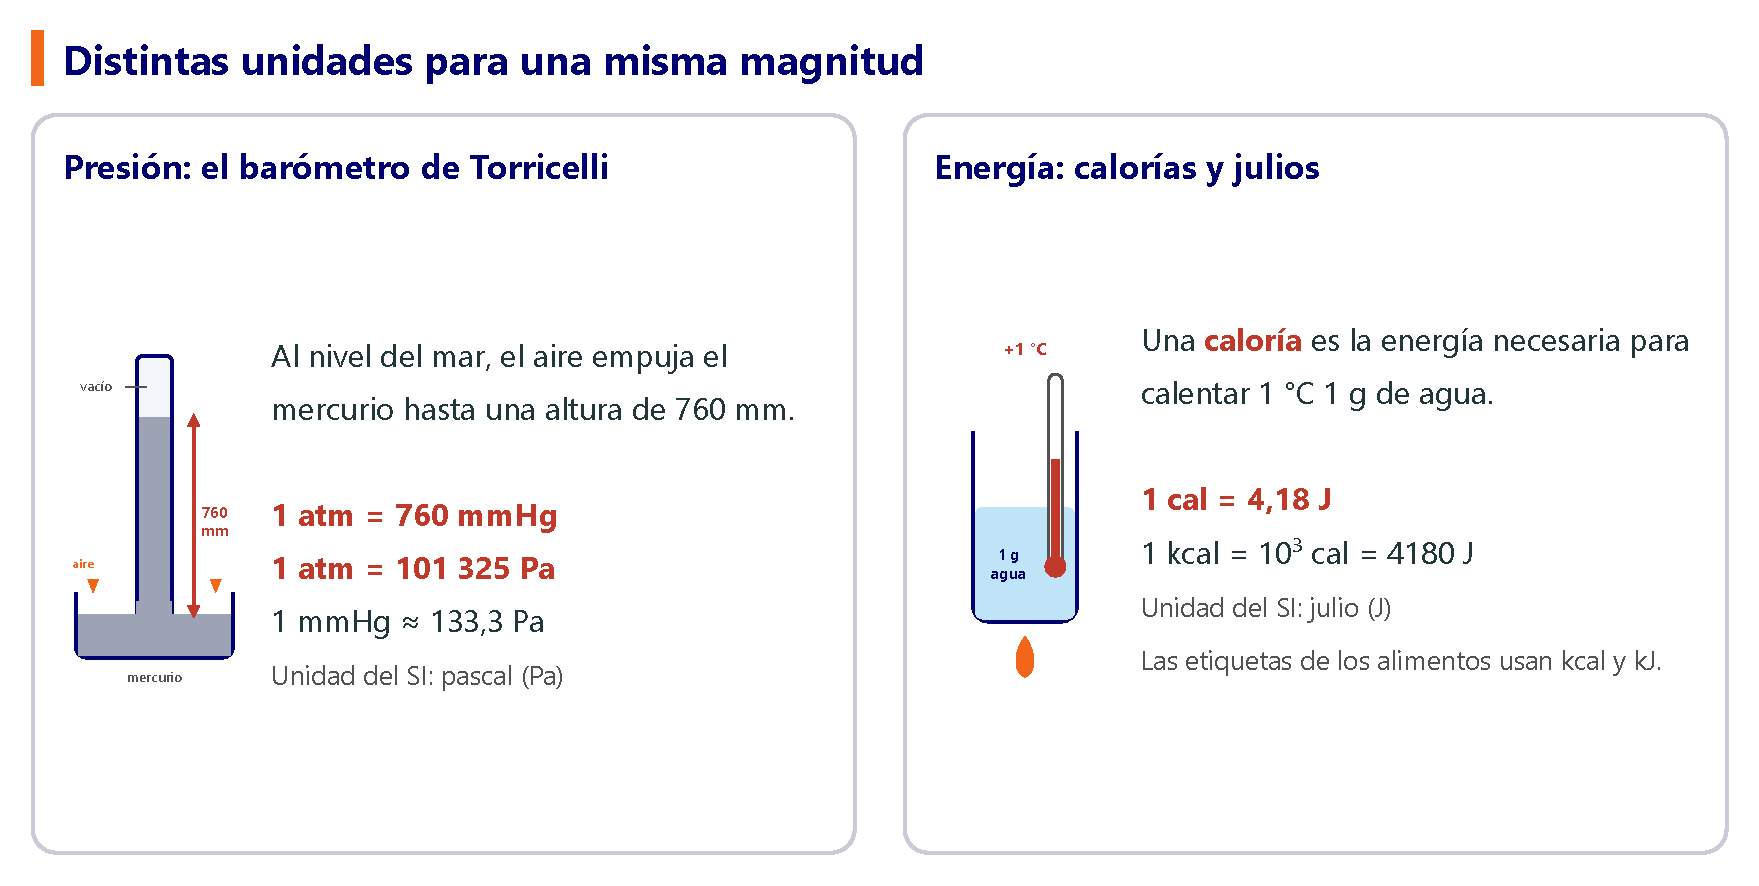
\includegraphics[width=\textwidth]{FigurasSVG/Unit_1_Matter_Measurement/pdf/pressure_energy_es.pdf}
    \caption{De dónde salen la atmósfera, el milímetro de mercurio y la caloría.}
    \label{fig:u1_pressure_energy}
\end{figure}

\begin{table}[H]
    \centering
    \renewcommand{\arraystretch}{1.4}
    \begin{tabular}{lcp{6.5cm}}
        \toprule
        \textbf{Magnitud} & \textbf{Unidad del SI} & \textbf{Equivalencias} \\
        \midrule
        Presión & pascal (\unit{\Pa}) & \(\qty{1}{\atmospher} = \qty{760}{\mmhg}\) \newline \(\qty{1}{\atmospher} = \qty{101325}{\Pa} \approx \qty{1.013e5}{\Pa}\) \\
        Energía & julio (\unit{\J}) & \(\qty{1}{\calorie} = \qty{4.18}{\J}\) \newline \(\qty{1}{\kilo\calorie} = \qty{e3}{\calorie}\) \\
        \bottomrule
    \end{tabular}
    \caption{Unidades de presión y de energía y sus equivalencias.}
    \label{tab:u1_pressure_energy}
\end{table}

\begin{example}
    \textbf{Presión.} La presión del aire de una rueda es \qty{1.5}{\atmospher}. Exprésala en \unit{\Pa} y en \unit{\mmhg}.
    \begin{equation*}
        \num{1.5}\,\cancelunit{\atmospher} \cdot \dfrac{\qty{101325}{\Pa}}{1\,\cancelunit{\atmospher}} \approx \textcolor{red}{\qty{1.52e5}{\Pa}}
        \qquad\qquad
        \num{1.5}\,\cancelunit{\atmospher} \cdot \dfrac{\qty{760}{\mmhg}}{1\,\cancelunit{\atmospher}} = \textcolor{red}{\qty{1140}{\mmhg}}
    \end{equation*}
\end{example}

\begin{example}
    \textbf{Presión.} Expresa \qty{380}{\mmhg} en pascales. No hay una equivalencia directa, así que pasamos por las atmósferas:
    \begin{equation*}
        \num{380}\,\cancelunit{\mmhg} \cdot \dfrac{1\,\cancelunit{\atmospher}}{\num{760}\,\cancelunit{\mmhg}} \cdot \dfrac{\qty{101325}{\Pa}}{1\,\cancelunit{\atmospher}} \approx \textcolor{red}{\qty{5.07e4}{\Pa}}
    \end{equation*}
\end{example}

\begin{example}
    \textbf{Energía.} Una barrita de chocolate aporta \qty{250}{\kilo\calorie}. Expresa esta energía en julios.
    \begin{equation*}
        \num{250}\,\cancelunit{\kilo\calorie} \cdot \dfrac{\num{e3}\,\cancelunit{\calorie}}{1\,\cancelunit{\kilo\calorie}} \cdot \dfrac{\qty{4.18}{\J}}{1\,\cancelunit{\calorie}} = \textcolor{red}{\qty{1.045e6}{\J}}
    \end{equation*}
\end{example}

\begin{exercise}
    Cambia de unidades estas presiones:
    \begin{enumerate}[label=\letraminuscula]
        \item \qty{0.33}{\atmospher} (presión del aire en la cima del Everest) a \unit{\mmhg}.
        \item \qty{120}{\mmhg} (una tensión arterial normal) a \unit{\atmospher} y a \unit{\Pa}.
        \item \qty{2e5}{\Pa} a \unit{\atmospher}.
    \end{enumerate}
    \begin{solu}
        \begin{enumerate}[label=\alph*)]
            \item \(\num{0.33}\,\unit{\atmospher} \cdot \dfrac{\qty{760}{\mmhg}}{\qty{1}{\atmospher}} \approx \qty{251}{\mmhg}\)
            \item \(\num{120}\,\unit{\mmhg} \cdot \dfrac{\qty{1}{\atmospher}}{\qty{760}{\mmhg}} \approx \qty{0.158}{\atmospher}\); \quad
            \(\num{120}\,\unit{\mmhg} \cdot \dfrac{\qty{1}{\atmospher}}{\qty{760}{\mmhg}} \cdot \dfrac{\qty{101325}{\Pa}}{\qty{1}{\atmospher}} \approx \qty{1.60e4}{\Pa}\)
            \item \(\num{2e5}\,\unit{\Pa} \cdot \dfrac{\qty{1}{\atmospher}}{\qty{101325}{\Pa}} \approx \qty{1.97}{\atmospher}\)
        \end{enumerate}
    \end{solu}
\end{exercise}

\begin{exercise}
    Cambia de unidades estas energías:
    \begin{enumerate}[label=\letraminuscula]
        \item \qty{836}{\J} a calorías.
        \item La etiqueta de un yogur indica \qty{400}{\kilo\joule}. Expresa esta energía en \unit{\kilo\calorie}.
        \item \qty{1.5}{\kilo\calorie} a \unit{\J}.
    \end{enumerate}
    \begin{solu}
        \begin{enumerate}[label=\alph*)]
            \item \(\num{836}\,\unit{\J} \cdot \dfrac{\qty{1}{\calorie}}{\qty{4.18}{\J}} = \qty{200}{\calorie}\)
            \item \(\num{400}\,\unit{\kilo\joule} \cdot \dfrac{\qty{e3}{\J}}{\qty{1}{\kilo\joule}} \cdot \dfrac{\qty{1}{\calorie}}{\qty{4.18}{\J}} \cdot \dfrac{\qty{1}{\kilo\calorie}}{\qty{e3}{\calorie}} \approx \qty{95.7}{\kilo\calorie}\)
            \item \(\num{1.5}\,\unit{\kilo\calorie} \cdot \dfrac{\qty{e3}{\calorie}}{\qty{1}{\kilo\calorie}} \cdot \dfrac{\qty{4.18}{\J}}{\qty{1}{\calorie}} = \qty{6270}{\J}\)
        \end{enumerate}
    \end{solu}
\end{exercise}

%----------------------------------------------------------------------------------------

\subsection{La notación científica}

% Calculator keys: \calckey{EXP} draws one key; \keys{3 . 2 EXP 3} draws one key per word
\providecommand{\calckey}[1]{{\setlength{\fboxsep}{1.5pt}\fbox{\footnotesize\sffamily\strut #1}}}
\ExplSyntaxOn
\providecommand{\keys}[1]{\seq_set_split:Nnn \l_tmpa_seq {~} {#1} \seq_map_inline:Nn \l_tmpa_seq {\calckey{##1}\,} \unskip}
\ExplSyntaxOff
% Red decimal comma used to show where the comma ends up in the examples
\providecommand{\redcomma}{\textcolor{red}{\mathbf{,}}}

En ciencia encontramos a menudo números muy grandes o muy pequeños. La distancia de la Tierra al Sol es de unos \qty{150000000}{\km}, y una bacteria mide unos \qty{0.000002}{\m}. Escribir y leer tantos ceros es lento y es muy fácil equivocarse. Por eso los científicos usan la \negsubro{notación científica}. Ya la has usado con los factores de conversión: \(\qty{1}{\km} = \qty{e3}{\m}\).

\begin{definition}[Notación científica]
    Es una forma de escribir un número como el producto de un \textbf{coeficiente} por una \textbf{potencia de 10}:
    \begin{equation*}
        a \cdot 10^{n}
    \end{equation*}
    \begin{itemize}
        \item El \textbf{coeficiente} \(a\) es un número del 1 al 9,99\ldots: tiene \textbf{una sola cifra, distinta de cero, delante de la coma decimal}.
        \item El \textbf{exponente} \(n\) es un número entero: \textbf{positivo} para los números mayores que 10 y \textbf{negativo} para los números menores que 1.
    \end{itemize}
\end{definition}

\begin{figure}[H]
    \centering
    % [FIGURA ORIGINAL] \includegraphics[width=\textwidth]{Unit_1/sci_notation_parts}
    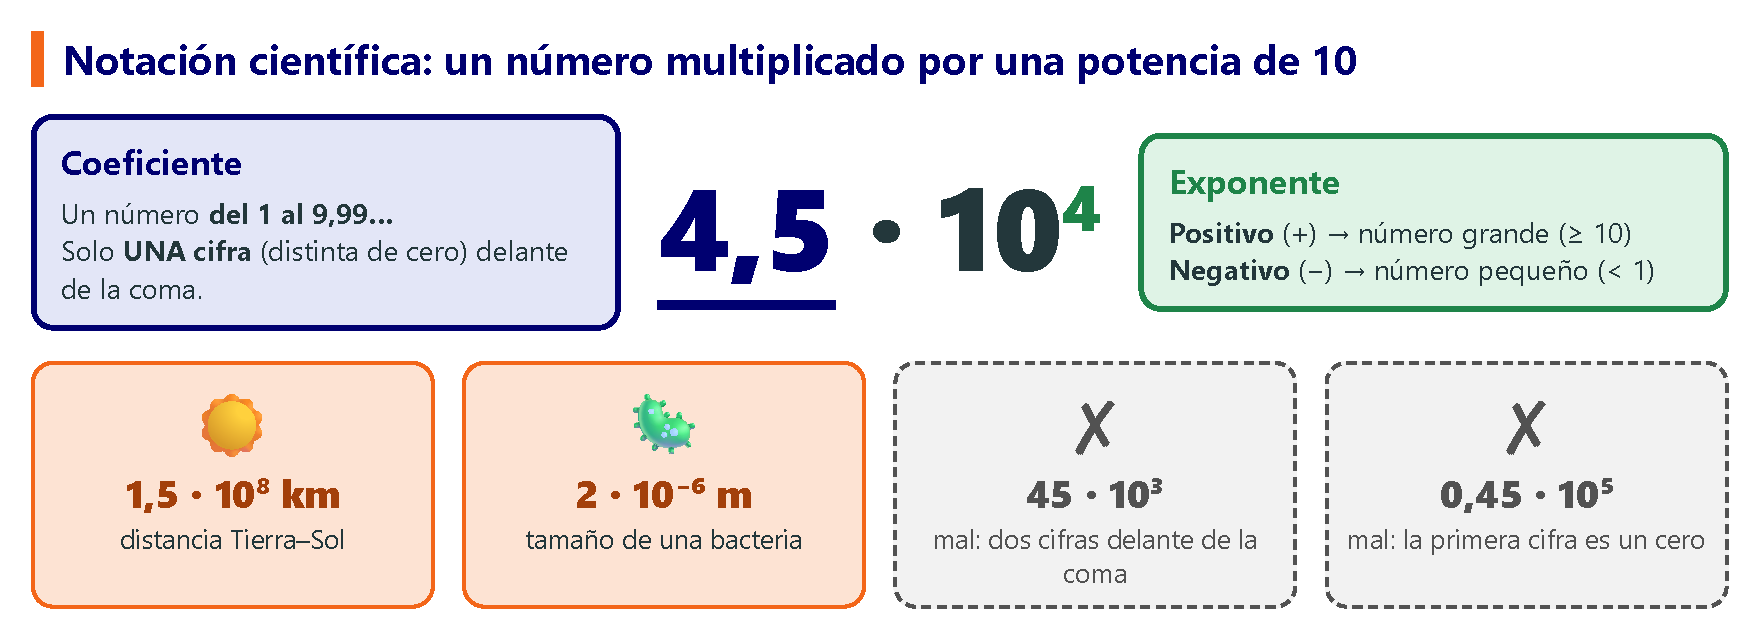
\includegraphics[width=\textwidth]{FigurasSVG/Unit_1_Matter_Measurement/pdf/sci_notation_parts_es.pdf}
    \caption{Las dos partes de un número en notación científica, con ejemplos correctos e incorrectos.}
    \label{fig:u1_sci_notation_parts}
\end{figure}

\begin{impt}
    \negsubro{¡La notación científica no cambia el número!} Es el \textbf{mismo número escrito de otra forma}, igual que «la mitad», \(\frac{1}{2}\) y \(0{,}5\) son la misma cantidad:
    \begin{equation*}
        45\,000 = 4{,}5 \cdot 10^{4} = 45 \cdot 10^{3} = 450 \cdot 10^{2} = 0{,}45 \cdot 10^{5}
    \end{equation*}
    Todas valen exactamente lo mismo. De todas estas formas de escribirlo, solo \(4{,}5 \cdot 10^{4}\) es \textbf{notación científica correcta}, porque tiene una sola cifra (distinta de cero) delante de la coma.
\end{impt}

Recuerda lo que significa una potencia de 10: el exponente nos dice cuántos lugares se mueve la coma.

\begin{table}[H]
    \centering
    \renewcommand{\arraystretch}{1.35}
    \begin{tabular}{cc@{\hspace{1.5cm}}cc}
        \toprule
        \textbf{Potencia} & \textbf{Decimal} & \textbf{Potencia} & \textbf{Decimal} \\
        \midrule
        \(10^{1}\) & \num{10}    & \(10^{-1}\) & \num{0.1}   \\
        \(10^{2}\) & \num{100}   & \(10^{-2}\) & \num{0.01}  \\
        \(10^{3}\) & \num{1000}  & \(10^{-3}\) & \num{0.001} \\
        \(10^{4}\) & \num{10000} & \(10^{-4}\) & \num{0.0001} \\
        \bottomrule
    \end{tabular}
    \caption{Las potencias de 10 positivas son números \textbf{mayores que 1}; las potencias de 10 negativas son números \textbf{menores que 1}. \(10^{0} = 1\).}
    \label{tab:u1_powers_of_ten}
\end{table}

\begin{figure}[H]
    \centering
    % [FIGURA ORIGINAL] \includegraphics[width=\textwidth]{Unit_1/sci_notation_to}
    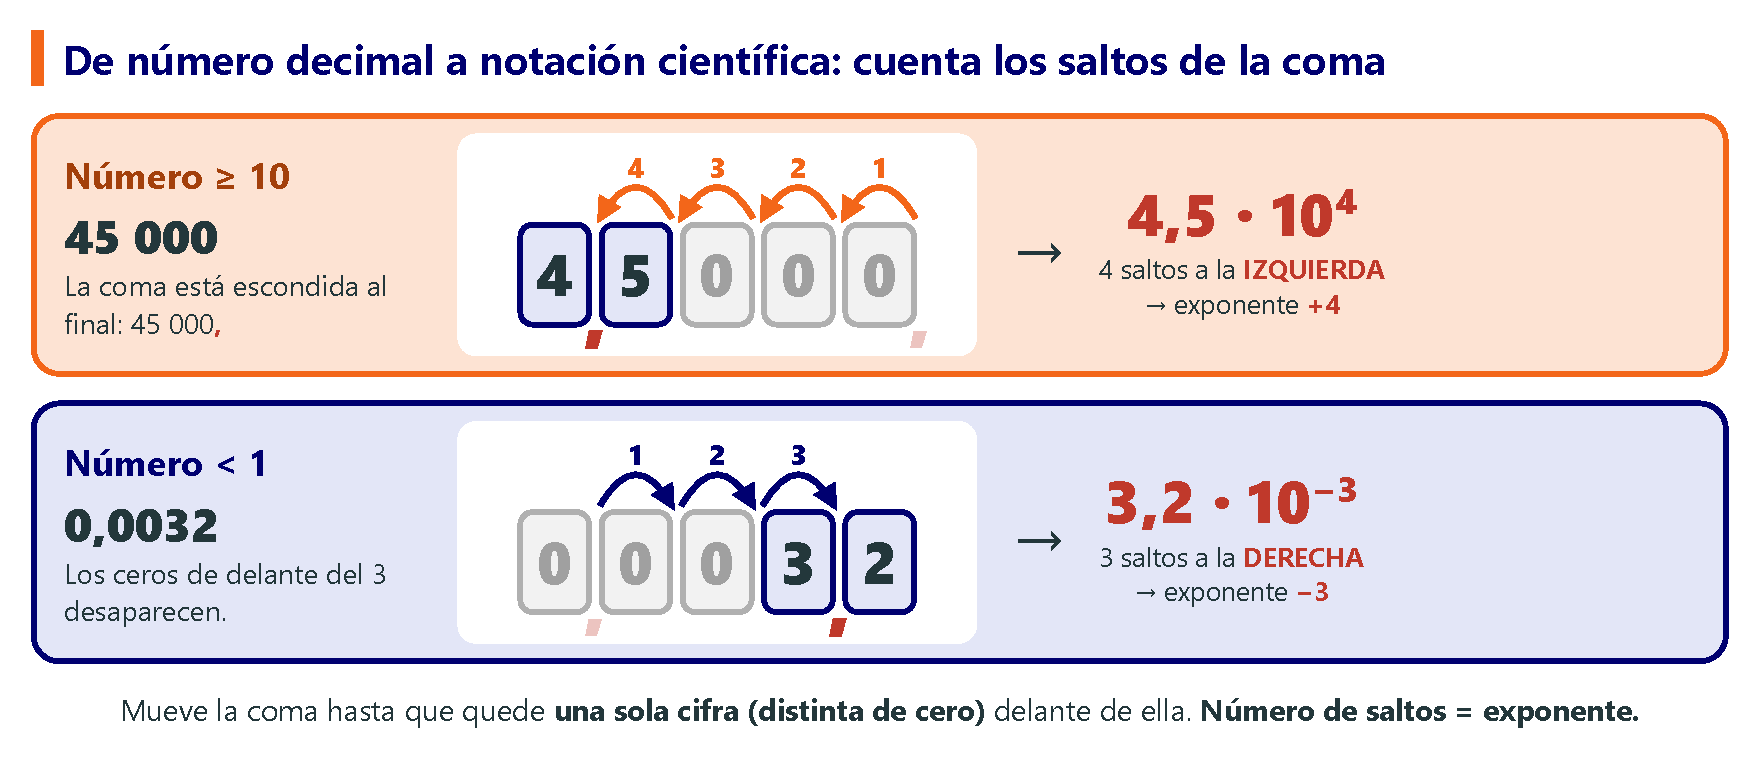
\includegraphics[width=\textwidth]{FigurasSVG/Unit_1_Matter_Measurement/pdf/sci_notation_to_es.pdf}
    \caption{Para escribir un número en notación científica contamos cuántos lugares salta la coma.}
    \label{fig:u1_sci_notation_to}
\end{figure}

%------------------------------------------------

\subsubsection{Números mayores que 1 en notación científica}

\negsubro{Método, paso a paso}:
\begin{enumerate}[label=\numberballmDarkTeal]
    \item Busca la coma decimal. Si el número no tiene coma, está \textbf{escondida al final}: \(45\,000 = 45\,000\redcomma\)
    \item Mueve la coma hacia la \textbf{izquierda}, de lugar en lugar, hasta que quede \textbf{una sola cifra} delante de ella. \textbf{Cuenta los saltos}.
    \item Escribe el \textbf{coeficiente}: las cifras con la coma en su nuevo sitio. Los ceros del final no hacen falta: \(4\redcomma 5000 = 4{,}5\).
    \item El \textbf{exponente} es el \textbf{número de saltos}, y es \textbf{positivo}: el número era grande.
    \item Comprueba: \(\num{4.5e4}\) tiene que ser igual al número de partida.
\end{enumerate}

\begin{example}
    \textbf{Escribe \num{45000} en notación científica.}
    \begin{enumerate}[label=\numberballmDarkTeal]
        \item Coma escondida al final: \(45\,000\redcomma\)
        \item Movemos la coma 4 lugares a la izquierda: \(45\,000\redcomma \to 4500\redcomma 0 \to 450\redcomma 00 \to 45\redcomma 000 \to 4\redcomma 5000\) \(\Rightarrow\) \textbf{4 saltos}.
        \item Coeficiente: \(4{,}5\).
        \item Exponente: \(+4\).
        \item \(\textcolor{red}{\num{45000} = \num{4.5e4}}\)
    \end{enumerate}
\end{example}

\begin{example}
    \textbf{Escribe \num{6700} y \num{380.5} en notación científica.}
    \begin{itemize}
        \item \(6700\redcomma \to 6\redcomma 700\): 3 saltos a la izquierda \(\Rightarrow\) \(\textcolor{red}{\num{6700} = \num{6.7e3}}\)
        \item \(380{,}5 \to 3\redcomma 805\): 2 saltos a la izquierda \(\Rightarrow\) \(\textcolor{red}{\num{380.5} = \num{3.805e2}}\)
    \end{itemize}
\end{example}

%------------------------------------------------

\subsubsection{Números menores que 1 en notación científica}

\negsubro{Método, paso a paso}:
\begin{enumerate}[label=\numberballmDarkTeal]
    \item Busca la coma decimal: \(0{,}0032\).
    \item Mueve la coma hacia la \textbf{derecha}, de lugar en lugar, hasta dejarla justo detrás de la \textbf{primera cifra distinta de cero}. \textbf{Cuenta los saltos}.
    \item Escribe el \textbf{coeficiente}: los ceros de delante desaparecen: \(0003\redcomma 2 = 3{,}2\).
    \item El \textbf{exponente} es el \textbf{número de saltos}, y es \textbf{negativo}: el número era menor que 1.
    \item Comprueba: \(\num{3.2e-3}\) tiene que ser igual al número de partida.
\end{enumerate}

\begin{example}
    \textbf{Escribe \num{0.0032} en notación científica.}
    \begin{enumerate}[label=\numberballmDarkTeal]
        \item Coma: \(0\redcomma 0032\)
        \item Movemos la coma 3 lugares a la derecha: \(0\redcomma 0032 \to 00\redcomma 032 \to 000\redcomma 32 \to 0003\redcomma 2\) \(\Rightarrow\) \textbf{3 saltos}.
        \item Coeficiente: \(3{,}2\).
        \item Exponente: \(-3\).
        \item \(\textcolor{red}{\num{0.0032} = \num{3.2e-3}}\)
    \end{enumerate}
\end{example}

\begin{example}
    \textbf{Escribe \num{0.07} y \num{0.125} en notación científica.}
    \begin{itemize}
        \item \(0{,}07 \to 007\redcomma\): 2 saltos a la derecha \(\Rightarrow\) \(\textcolor{red}{\num{0.07} = \num{7e-2}}\)
        \item \(0{,}125 \to 01\redcomma 25\): 1 salto a la derecha \(\Rightarrow\) \(\textcolor{red}{\num{0.125} = \num{1.25e-1}}\)
    \end{itemize}
\end{example}

\begin{impt}
    \textbf{¿Hacia dónde se mueve la coma?}
    \begin{itemize}
        \item Número grande (mayor que 10) \(\to\) la coma salta a la \textbf{izquierda} \(\to\) exponente \textbf{positivo}.
        \item Número pequeño (menor que 1) \(\to\) la coma salta a la \textbf{derecha} \(\to\) exponente \textbf{negativo}.
        \item Número entre 1 y 10 \(\to\) la coma no se mueve \(\to\) exponente \textbf{0}: \(7{,}2 = \num{7.2e0}\).
    \end{itemize}
\end{impt}

%------------------------------------------------

\subsubsection{De notación científica a número decimal}

Ahora hacemos lo contrario: partimos de \(a \cdot 10^{n}\) y queremos el número normal (decimal). El \textbf{exponente} nos dice cuántos lugares salta la coma, y su \textbf{signo} nos dice hacia dónde.

\begin{figure}[H]
    \centering
    % [FIGURA ORIGINAL] \includegraphics[width=\textwidth]{Unit_1/sci_notation_back}
    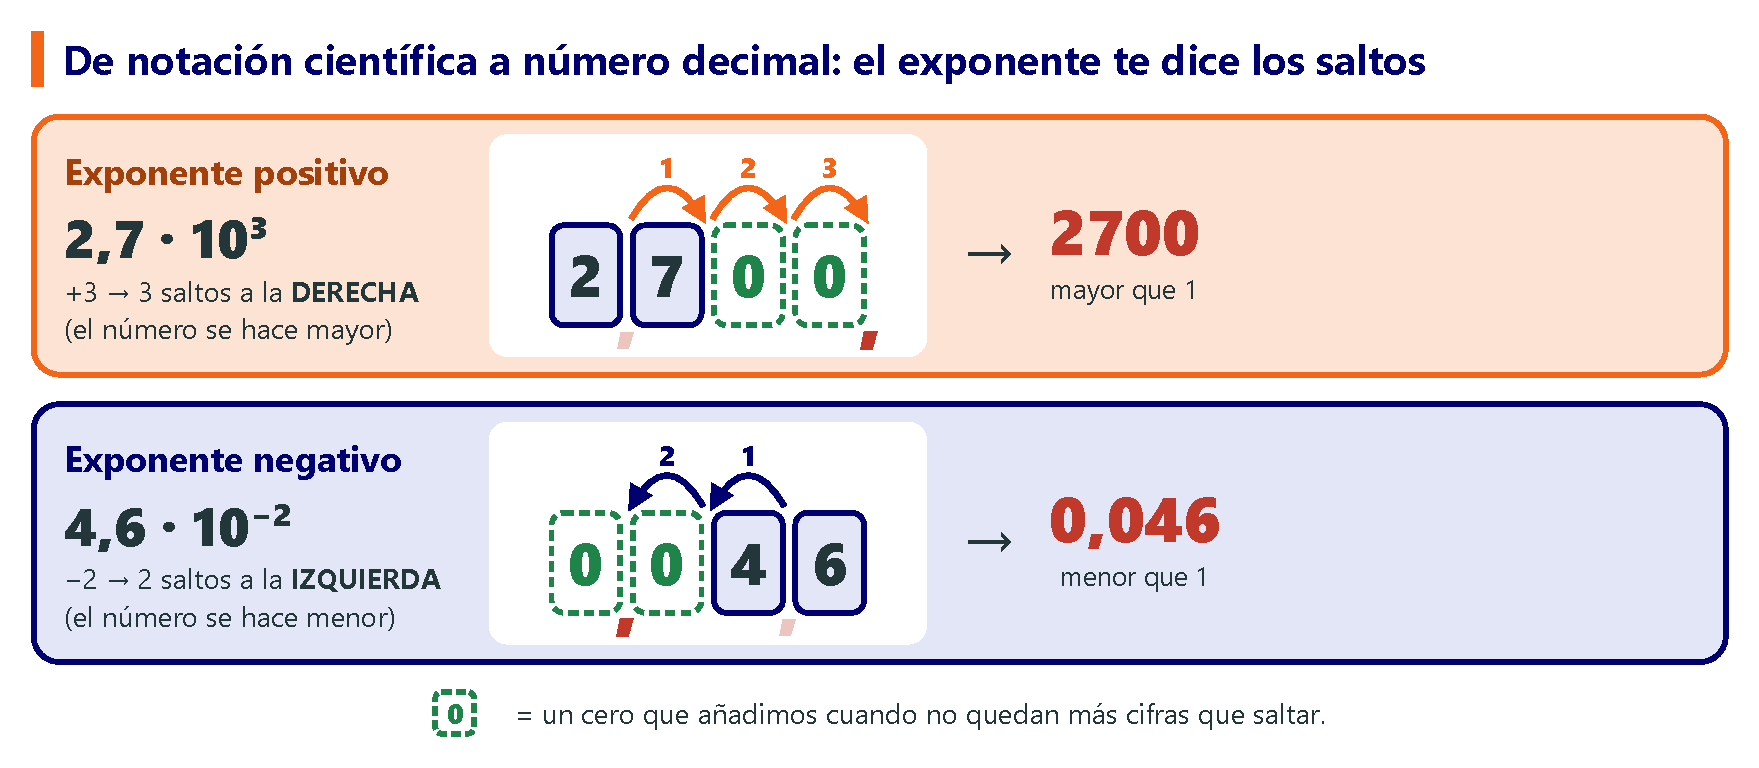
\includegraphics[width=\textwidth]{FigurasSVG/Unit_1_Matter_Measurement/pdf/sci_notation_back_es.pdf}
    \caption{De notación científica a número decimal: con exponente positivo, la coma salta a la derecha; con exponente negativo, la coma salta a la izquierda.}
    \label{fig:u1_sci_notation_back}
\end{figure}

\negsubro{Método, paso a paso}:
\begin{enumerate}[label=\numberballmDarkTeal]
    \item Mira el \textbf{signo del exponente}:
    \begin{itemize}
        \item \textbf{Positivo} \(\to\) la coma salta a la \textbf{derecha} (el número se hace \textbf{mayor}).
        \item \textbf{Negativo} \(\to\) la coma salta a la \textbf{izquierda} (el número se hace \textbf{menor}).
    \end{itemize}
    \item Mueve la coma tantos lugares como indique el exponente.
    \item Si no quedan más cifras que saltar, \textbf{añade ceros}.
    \item Si la coma queda delante del todo, escribe un \textbf{0} delante: \(\redcomma 046 \to 0{,}046\).
\end{enumerate}

\begin{example}
    \textbf{Exponente positivo: escribe \num{2.7e3} como número decimal.}
    \begin{enumerate}[label=\numberballmDarkTeal]
        \item Exponente \(+3\): 3 saltos a la \textbf{derecha}.
        \item \(2\redcomma 7 \to 27\redcomma \to 270\redcomma \to 2700\redcomma\) (hemos añadido dos ceros).
        \item \(\textcolor{red}{\num{2.7e3} = \num{2700}}\)
    \end{enumerate}
    Más ejemplos: \(\num{5e2} = 500\); \quad \(\num{1.25e3} = 1250\); \quad \(\num{3.06e4} = \num{30600}\).
\end{example}

\begin{example}
    \textbf{Exponente negativo: escribe \num{4.6e-2} como número decimal.}
    \begin{enumerate}[label=\numberballmDarkTeal]
        \item Exponente \(-2\): 2 saltos a la \textbf{izquierda}.
        \item \(4\redcomma 6 \to \redcomma 46 \to \redcomma 046\) (hemos añadido un cero).
        \item Escribimos un 0 delante de la coma: \(\textcolor{red}{\num{4.6e-2} = \num{0.046}}\)
    \end{enumerate}
    Más ejemplos: \(\num{8e-3} = \num{0.008}\); \quad \(\num{1.5e-1} = \num{0.15}\); \quad \(\num{9.2e-4} = \num{0.00092}\).
\end{example}

\begin{marker}
    \textbf{Comprobación rápida}: si el exponente es positivo, tu número decimal tiene que ser \textbf{mayor que 1}; si es negativo, tiene que empezar por \textbf{0,\ldots}. Si no, ¡has movido la coma hacia el lado equivocado!
\end{marker}

\begin{exercise}
    Escribe estos números en notación científica:
    \begin{enumerate}[label=\letraminuscula]
        \item \num{3400}
        \item \num{52000}
        \item \num{700000}
        \item \num{186}
        \item \num{0.045}
        \item \num{0.0007}
        \item \num{0.00128}
        \item \num{0.5}
    \end{enumerate}
    \begin{solu}
        \begin{enumerate}[label=\alph*)]
            \item 3 saltos a la izquierda: \(\num{3.4e3}\)
            \item 4 saltos a la izquierda: \(\num{5.2e4}\)
            \item 5 saltos a la izquierda: \(\num{7e5}\)
            \item 2 saltos a la izquierda: \(\num{1.86e2}\)
            \item 2 saltos a la derecha: \(\num{4.5e-2}\)
            \item 4 saltos a la derecha: \(\num{7e-4}\)
            \item 3 saltos a la derecha: \(\num{1.28e-3}\)
            \item 1 salto a la derecha: \(\num{5e-1}\)
        \end{enumerate}
    \end{solu}
\end{exercise}

\begin{exercise}
    Escribe estos números como números decimales:
    \begin{enumerate}[label=\letraminuscula]
        \item \num{3.1e2}
        \item \num{6e4}
        \item \num{1.25e3}
        \item \num{9e-1}
        \item \num{2.4e-3}
        \item \num{7.05e-2}
    \end{enumerate}
    \begin{solu}
        \begin{enumerate}[label=\alph*)]
            \item 2 saltos a la derecha: \num{310}
            \item 4 saltos a la derecha: \num{60000}
            \item 3 saltos a la derecha: \num{1250}
            \item 1 salto a la izquierda: \num{0.9}
            \item 3 saltos a la izquierda: \num{0.0024}
            \item 2 saltos a la izquierda: \num{0.0705}
        \end{enumerate}
    \end{solu}
\end{exercise}

\begin{exercise}
    Estos números \textbf{no} están bien escritos en notación científica. Explica el error y escríbelos correctamente: \num{23e4}, \num{0.8e3}, \num{15e-3}.
    \begin{solu}
        \begin{itemize}
            \item \(\num{23e4}\): hay dos cifras delante de la coma. \(\num{23e4} = \num{230000} = \num{2.3e5}\).
            \item \(\num{0.8e3}\): la cifra de delante de la coma es un cero. \(\num{0.8e3} = \num{800} = \num{8e2}\).
            \item \(\num{15e-3}\): hay dos cifras delante de la coma. \(\num{15e-3} = \num{0.015} = \num{1.5e-2}\).
        \end{itemize}
    \end{solu}
\end{exercise}

\begin{exercise}
    Escribe en notación científica los números de estas frases:
    \begin{enumerate}[label=\letraminuscula]
        \item El sonido viaja por el aire a \qty{340}{\m\per\s}.
        \item Un pelo humano tiene un grosor de unos \qty{0.00008}{\m}.
        \item La Luna está a unos \qty{384000}{\km} de la Tierra.
        \item Un grano de arena tiene una masa de unos \qty{0.0006}{\g}.
    \end{enumerate}

    \begin{solu}
        \begin{enumerate}[label=\alph*)]
            \item \(\qty{3.4e2}{\m\per\s}\)
            \item \(\qty{8e-5}{\m}\)
            \item \(\qty{3.84e5}{\km}\)
            \item \(\qty{6e-4}{\g}\)
        \end{enumerate}
    \end{solu}
\end{exercise}

\begin{exercise}
    Escribe estos números en notación científica. Cuidado: los cuatro últimos ya tienen una potencia de 10, pero \textbf{todavía no} están bien escritos.
    \begin{enumerate}[label=\letraminuscula]
        \item \num{4569201}
        \item \num{0.0026}
        \item \num{235.78}
        \item \num{500000}
        \item \num{4055e4}
        \item \num{5687e-8}
        \item \num{253e8}
        \item \num{0.0254e-2}
    \end{enumerate}
    \begin{solu}
        \begin{enumerate}[label=\alph*)]
            \item 6 saltos a la izquierda: \(\num{4.569201e6}\)
            \item 3 saltos a la derecha: \(\num{2.6e-3}\)
            \item 2 saltos a la izquierda: \(\num{2.3578e2}\)
            \item 5 saltos a la izquierda: \(\num{5e5}\)
            \item \(4055 = \num{4.055e3}\), así que \(\num{4055e4} = \num{4.055e3} \cdot 10^{4} = \num{4.055e7}\)
            \item \(5687 = \num{5.687e3}\), así que \(\num{5687e-8} = \num{5.687e3} \cdot 10^{-8} = \num{5.687e-5}\)
            \item \(253 = \num{2.53e2}\), así que \(\num{253e8} = \num{2.53e2} \cdot 10^{8} = \num{2.53e10}\)
            \item \(0{,}0254 = \num{2.54e-2}\), así que \(\num{0.0254e-2} = \num{2.54e-2} \cdot 10^{-2} = \num{2.54e-4}\)
        \end{enumerate}
    \end{solu}
\end{exercise}

%------------------------------------------------

\subsubsection{La notación científica en la calculadora}

Todas las calculadoras científicas tienen una tecla especial para escribir una potencia de 10. Según lo antigua que sea la calculadora, se llama \textbf{EXP} o \(\boldsymbol{\times 10^{x}}\), pero hace exactamente lo mismo: significa «\(\times\,10\) elevado a». Busca tu calculadora en la figura y sigue las teclas.

\begin{figure}[H]
    \centering
    % [FIGURA ORIGINAL] \includegraphics[width=\textwidth]{Unit_1/calculators_sci}
    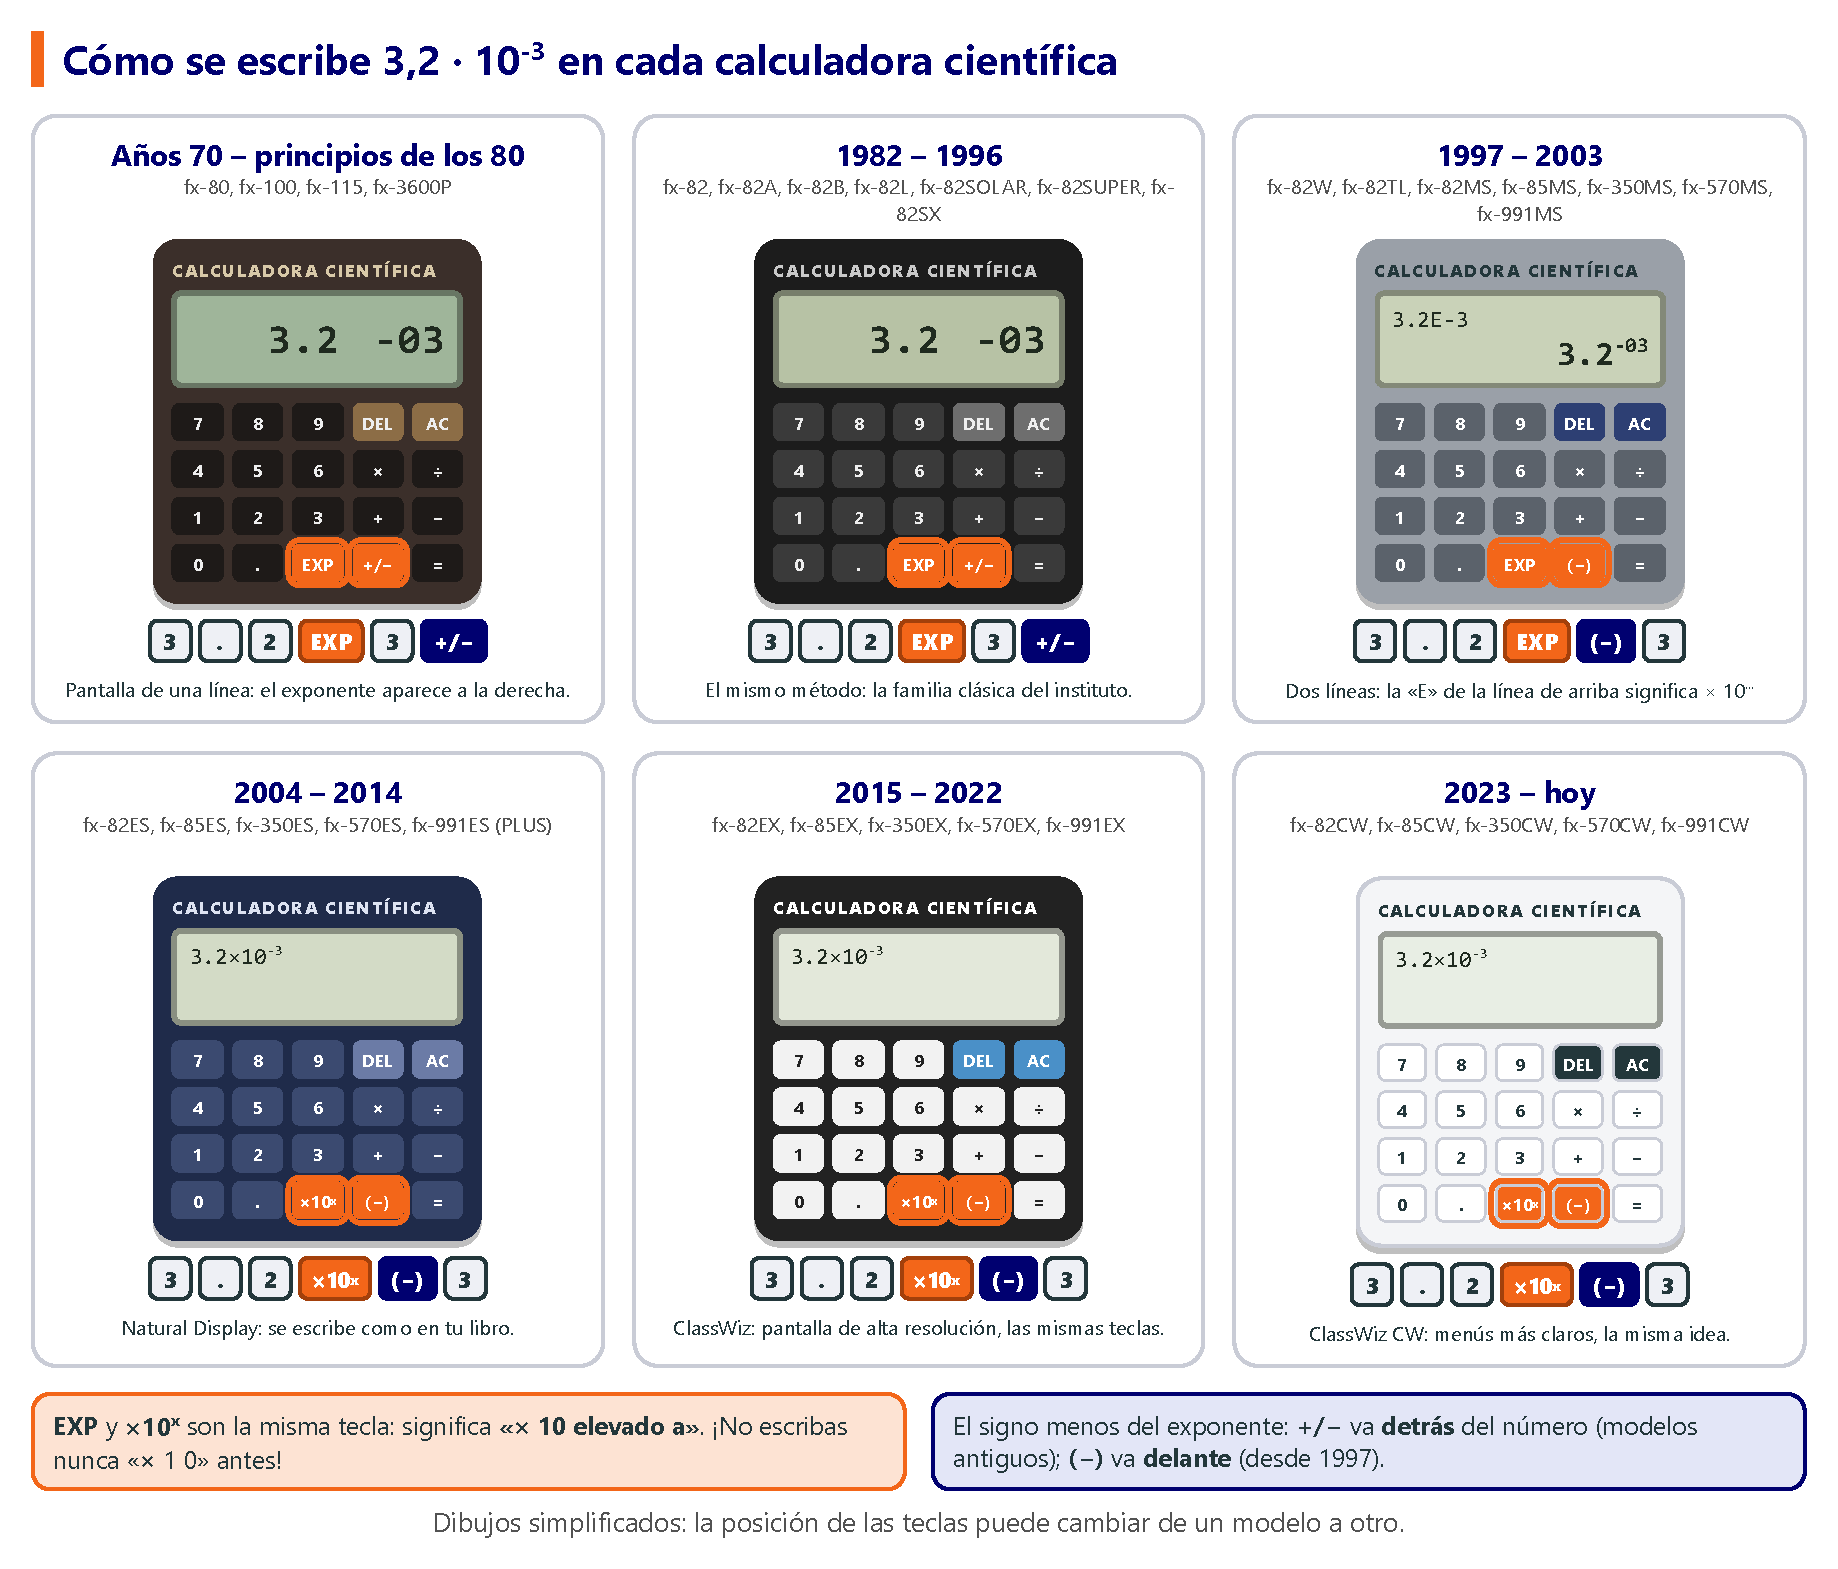
\includegraphics[width=\textwidth]{FigurasSVG/Unit_1_Matter_Measurement/pdf/calculators_sci_es.pdf}
    \caption{Cómo se escribe \(\num{3.2e-3}\) en las calculadoras científicas que se han usado en los institutos a lo largo de los años (dibujos simplificados).}
    \label{fig:u1_calculators_sci}
\end{figure}

\begin{table}[H]
    \centering
    \small
    \renewcommand{\arraystretch}{1.35}
    \begin{tabular}{p{1.9cm}p{4.0cm}p{2.9cm}p{3.7cm}}
        \toprule
        \textbf{Años} & \textbf{Modelos más habituales} & \textbf{Teclas} & \textbf{Para escribir \(\num{3.2e-3}\)} \\
        \midrule
        Años 70--principios de los 80 & fx-80, fx-100, fx-115, fx-3600P & \calckey{EXP} y \calckey{+/\(-\)} & \keys{3 . 2 EXP 3 +/-} \\
        1982--1996 & fx-82, fx-82A, fx-82B, fx-82L, fx-82SOLAR, fx-82SUPER, fx-82SX & \calckey{EXP} y \calckey{+/\(-\)} & \keys{3 . 2 EXP 3 +/-} \\
        1997--2003 & fx-82W, fx-82TL, fx-82MS, fx-85W, fx-85MS, fx-115W, fx-115MS, fx-350MS, fx-570MS, fx-991MS & \calckey{EXP} y \calckey{(\(-\))} & \keys{3 . 2 EXP (-) 3} \\
        2004--2014 & fx-82ES, fx-85ES, fx-350ES, fx-570ES, fx-991ES, fx-82ES PLUS, fx-991ES PLUS & \calckey{\(\times10^{x}\)} y \calckey{(\(-\))} & \keys{3 . 2 \(\times10^{x}\) (-) 3} \\
        2015--2022 & fx-82EX, fx-85EX, fx-350EX, fx-570EX, fx-991EX (y 2.ª edición) & \calckey{\(\times10^{x}\)} y \calckey{(\(-\))} & \keys{3 . 2 \(\times10^{x}\) (-) 3} \\
        2023--hoy & fx-82CW, fx-85CW, fx-350CW, fx-570CW, fx-991CW & \calckey{\(\times10^{x}\)} y \calckey{(\(-\))} & \keys{3 . 2 \(\times10^{x}\) (-) 3} \\
        \bottomrule
    \end{tabular}
    \caption{La tecla de la notación científica en las calculadoras escolares más habituales.}
    \label{tab:u1_calculators}
\end{table}

\begin{example}
    \textbf{Escribe \(\num{6.02e23}\)} (el exponente es positivo, así que no hace falta el signo menos):
    \begin{itemize}
        \item Calculadoras hasta 2003: \keys{6 . 0 2 EXP 2 3}. En la pantalla verás \texttt{6.02E23} o \(6.02^{23}\).
        \item Calculadoras desde 2004: \keys{6 . 0 2 \(\times10^{x}\) 2 3}. En la pantalla verás \(6.02 \times 10^{23}\).
    \end{itemize}
\end{example}

\begin{marker}
    \textbf{Error típico}: \textbf{no} pulses \keys{\(\times\) 1 0} antes de la tecla EXP o \(\times 10^{x}\), porque la tecla ya incluye el «\(\times\,10\)». Si tecleas \keys{3 . 2 \(\times\) 1 0 EXP (-) 3}, la calculadora entiende \(3{,}2 \cdot 10 \cdot 10^{-3}\), ¡que es 10 veces más grande! Del mismo modo, para escribir \(10^{5}\) solo, pulsa \keys{1 EXP 5}, no \keys{1 0 EXP 5}.
\end{marker}

\begin{exercise}
    Escribe las teclas que pulsarías en \textbf{tu propia} calculadora para escribir estos números, y compruébalos en la pantalla: \textbf{a)} \(\num{5.4e6}\); \textbf{b)} \(\num{7.1e-4}\); \textbf{c)} \(\num{1.6e-19}\); \textbf{d)} \(\num{3e8}\).
    \begin{solu}
        Con una calculadora de 2004 en adelante (con las más antiguas, usa EXP en lugar de \(\times 10^{x}\); antes de 1997, pulsa \(+/-\) después del exponente en lugar de \((-)\) antes de él):
        a) \keys{5 . 4 \(\times10^{x}\) 6}; b) \keys{7 . 1 \(\times10^{x}\) (-) 4}; c) \keys{1 . 6 \(\times10^{x}\) (-) 1 9}; d) \keys{3 \(\times10^{x}\) 8}.
    \end{solu}
\end{exercise}


\section{La densidad y la flotación}


\begin{definition}[Densidad]
    Es la masa que hay en cada unidad de volumen de una sustancia:
    \begin{equation*}
        d = \dfrac{m}{V}
    \end{equation*}
\end{definition}

\begin{figure}[H]
    \centering
    % [FIGURA ORIGINAL] \includegraphics[width=\textwidth]{Unit_1/density_cubes}
    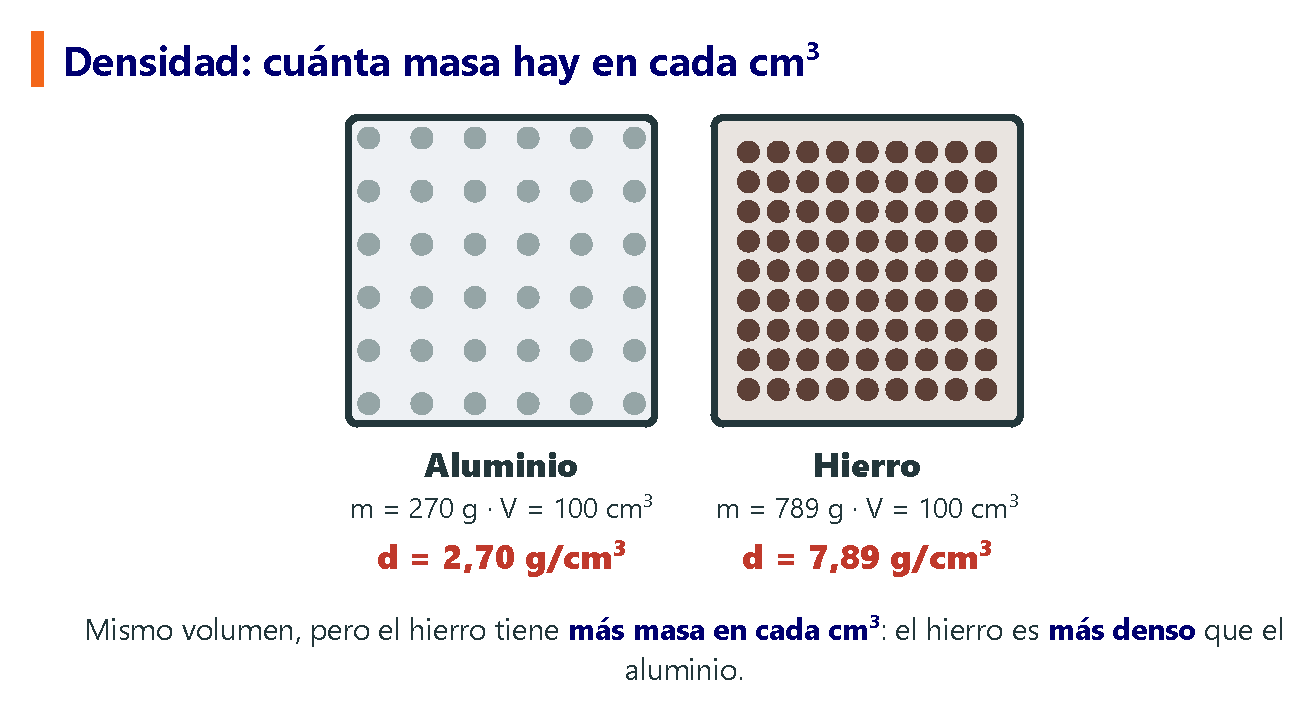
\includegraphics[width=\textwidth]{FigurasSVG/Unit_1_Matter_Measurement/pdf/density_cubes_es.pdf}
    \caption{Dos cubos con el mismo volumen pero distinta masa tienen distinta densidad.}
    \label{fig:u1_density_cubes}
\end{figure}

\negsubro{Cómo despejar una magnitud en la fórmula de la densidad}

La fórmula \(d = \dfrac{m}{V}\) relaciona tres magnitudes. Si conocemos \textbf{dos} de ellas, siempre podemos calcular la \textbf{tercera}. Pero antes tenemos que dejar la magnitud que queremos calcular \textbf{sola} en un lado del signo igual. Esto se llama \textbf{despejar} una magnitud.

La idea clave es que una ecuación es como una \textbf{balanza en equilibrio}: lo que hagamos en un lado lo tenemos que hacer también en el otro, para que los dos lados sigan siendo iguales.

\begin{figure}[H]
    \centering
    % [FIGURA ORIGINAL] \includegraphics[width=\textwidth]{Unit_1/density_isolate}
    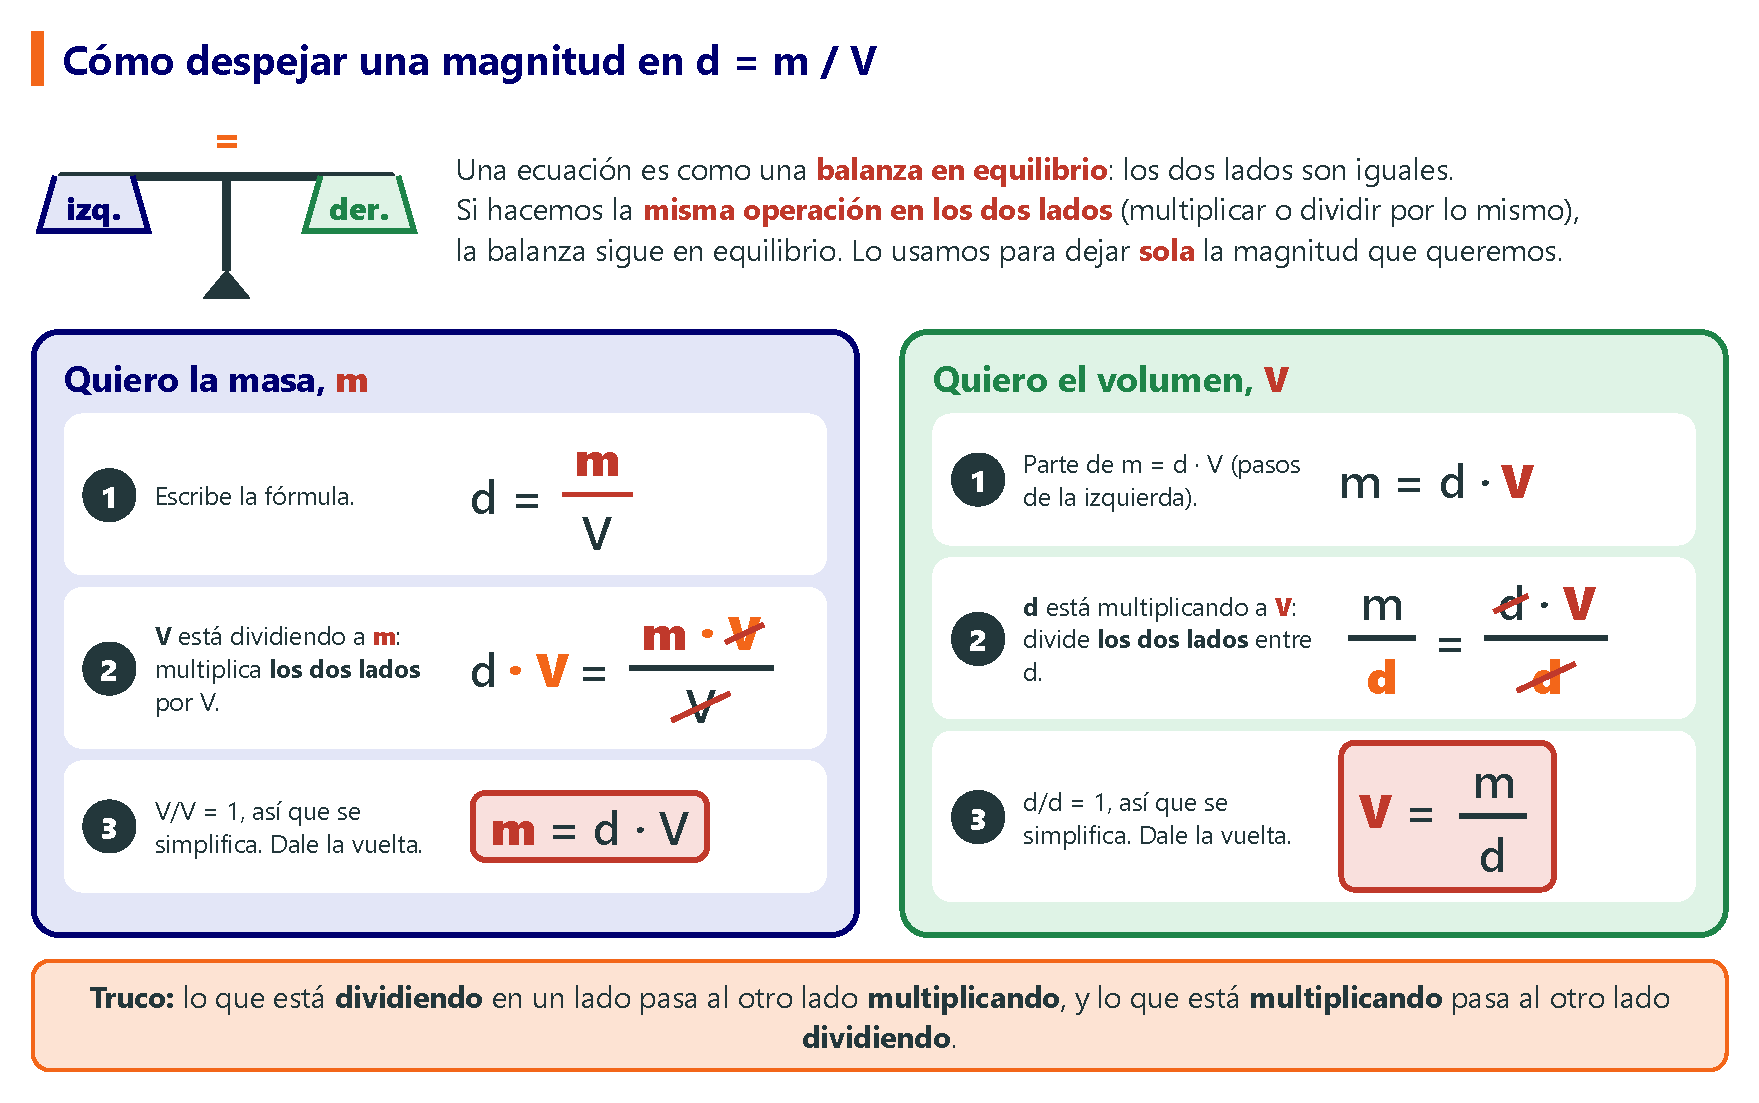
\includegraphics[width=\textwidth]{FigurasSVG/Unit_1_Matter_Measurement/pdf/density_isolate_es.pdf}
    \caption{Cómo despejar la masa y el volumen en la fórmula de la densidad, paso a paso.}
    \label{fig:u1_density_isolate}
\end{figure}

\negsubro{Método, paso a paso}:
\begin{enumerate}[label=\numberballmDarkTeal]
    \item Lee el ejercicio y escribe los \textbf{datos} con sus unidades. Subraya la magnitud que pide el ejercicio (la \textbf{incógnita}).
    \item Escribe la fórmula \(d = \dfrac{m}{V}\).
    \item Mira qué hay \textbf{junto a} la incógnita y haz la \textbf{operación contraria en los dos lados}:
    \begin{itemize}
        \item Si la incógnita está \textbf{dividida} por algo, \textbf{multiplica} los dos lados por eso.
        \item Si la incógnita está \textbf{multiplicada} por algo, \textbf{divide} los dos lados entre eso.
    \end{itemize}
    \item Simplifica lo que se repite arriba y abajo (vale 1) y escribe la incógnita a la izquierda: \(m = d \cdot V\) o \(V = \dfrac{m}{d}\).
    \item Sustituye los números \textbf{con sus unidades}, calcula y comprueba que la unidad del resultado tiene sentido.
\end{enumerate}

\begin{impt}
    Las tres versiones de la misma fórmula:
    \begin{equation*}
        d = \dfrac{m}{V} \qquad\qquad m = d \cdot V \qquad\qquad V = \dfrac{m}{d}
    \end{equation*}
    \textbf{Truco}: lo que está \textbf{dividiendo} en un lado pasa al otro lado \textbf{multiplicando}, y lo que está \textbf{multiplicando} pasa al otro lado \textbf{dividiendo}.
\end{impt}

\begin{example}
    \textbf{Cálculo de una masa.} Un anillo de oro tiene un volumen de \qty{0.8}{\cubic\cm}. La densidad del oro es \qty{19.3}{\g\per\cubic\cm}. ¿Cuál es la masa del anillo?
    \begin{enumerate}[label=\numberballmDarkTeal]
        \item Datos: \(V = \qty{0.8}{\cubic\cm}\), \(d = \qty{19.3}{\g\per\cubic\cm}\). Incógnita: \(\underline{m}\).
        \item Fórmula: \(d = \dfrac{m}{V}\).
        \item \(m\) está dividida por \(V\), así que multiplicamos los dos lados por \(V\):
        \(\;d \cdot V = \dfrac{m \cdot \cancelred{V}}{\cancelred{V}}\)
        \item \(m = d \cdot V\)
        \item \(m = \qty{19.3}{\g\per\cubic\cm} \cdot \qty{0.8}{\cubic\cm} = \textcolor{red}{\qty{15.44}{\g}}\)
    \end{enumerate}
\end{example}

\begin{example}
    \textbf{Cálculo de un volumen.} Queremos echar \qty{500}{\g} de aceite de oliva en una jarra. La densidad del aceite de oliva es \qty{0.92}{\g\per\mL}. ¿Qué volumen de aceite es?
    \begin{enumerate}[label=\numberballmDarkTeal]
        \item Datos: \(m = \qty{500}{\g}\), \(d = \qty{0.92}{\g\per\mL}\). Incógnita: \(\underline{V}\).
        \item Fórmula: \(d = \dfrac{m}{V}\). Primero subimos \(V\) (está dividiendo, así que pasa al otro lado multiplicando): \(m = d \cdot V\).
        \item \(V\) está multiplicado por \(d\), así que dividimos los dos lados entre \(d\):
        \(\;\dfrac{m}{d} = \dfrac{\cancelred{d} \cdot V}{\cancelred{d}}\)
        \item \(V = \dfrac{m}{d}\)
        \item \(V = \dfrac{\qty{500}{\g}}{\qty{0.92}{\g\per\mL}} \approx \textcolor{red}{\qty{543}{\mL}}\)
    \end{enumerate}
\end{example}

\begin{exercise}
    Despeja la incógnita y calcula:
    \begin{enumerate}[label=\letraminuscula]
        \item La masa de \qty{250}{\mL} de leche (\(d = \qty{1.03}{\g\per\mL}\)).
        \item El volumen de \qty{100}{\g} de mercurio (\(d = \qty{13.6}{\g\per\mL}\)).
        \item La masa de un cubito de hielo de \qty{30}{\cubic\cm} (\(d = \qty{0.92}{\g\per\cubic\cm}\)).
        \item El volumen de una pieza de aluminio de \qty{54}{\g} (\(d = \qty{2.70}{\g\per\cubic\cm}\)).
    \end{enumerate}
    \begin{solu}
        \begin{enumerate}[label=\alph*)]
            \item \(m = d \cdot V = \qty{1.03}{\g\per\mL} \cdot \qty{250}{\mL} = \qty{257.5}{\g}\)
            \item \(V = \dfrac{m}{d} = \dfrac{\qty{100}{\g}}{\qty{13.6}{\g\per\mL}} \approx \qty{7.35}{\mL}\)
            \item \(m = d \cdot V = \qty{0.92}{\g\per\cubic\cm} \cdot \qty{30}{\cubic\cm} = \qty{27.6}{\g}\)
            \item \(V = \dfrac{m}{d} = \dfrac{\qty{54}{\g}}{\qty{2.70}{\g\per\cubic\cm}} = \qty{20}{\cubic\cm}\)
        \end{enumerate}
    \end{solu}
\end{exercise}

\begin{exercise}
    El mismo método sirve para cualquier fórmula del tipo \(a = \dfrac{b}{c}\). La velocidad de una ciclista es \(v = \dfrac{s}{t}\), donde \(s\) es la distancia y \(t\) el tiempo.
    \begin{enumerate}[label=\letraminuscula]
        \item Despeja \(s\) y \(t\), explicando la operación que haces en cada paso.
        \item Una ciclista va a \qty{5}{\m\per\s} durante \qty{120}{\s}. ¿Qué distancia recorre?
        \item ¿Cuánto tarda en recorrer \qty{1500}{\m} a la misma velocidad?
    \end{enumerate}
    \begin{solu}
        \begin{enumerate}[label=\alph*)]
            \item \(s\) está dividida por \(t\): multiplicamos los dos lados por \(t\) \(\to\) \(s = v \cdot t\). Después, \(t\) está multiplicado por \(v\): dividimos los dos lados entre \(v\) \(\to\) \(t = \dfrac{s}{v}\).
            \item \(s = v \cdot t = \qty{5}{\m\per\s} \cdot \qty{120}{\s} = \qty{600}{\m}\)
            \item \(t = \dfrac{s}{v} = \dfrac{\qty{1500}{\m}}{\qty{5}{\m\per\s}} = \qty{300}{\s}\)
        \end{enumerate}
    \end{solu}
\end{exercise}

\begin{exercise}
    Un vaso contiene \qty{50}{\cmcubicos} de aceite y \qty{120}{\cmcubicos} de agua a \qty{20}{\celsius}. El aceite es amarillo, no se disuelve en agua y flota porque su densidad (\qty{0.9}{\g\per\mL}) es menor que la del agua (\qty{1.0}{\g\per\mL}).
    \begin{enumerate}[label=\letraminuscula]
        \item Enumera todas las propiedades de la materia que aparecen en el texto.
        \item Clasifica cada propiedad como cuantitativa/cualitativa y como extensiva/intensiva.
    \end{enumerate}
    \begin{solu}
        \begin{enumerate}[label=\alph*)]
            \item Volumen de aceite, volumen de agua, color del aceite, solubilidad del aceite en agua, densidad del aceite, densidad del agua, temperatura.
            \item Volúmenes: \textbf{cuantitativas, extensivas}. Temperatura: \textbf{cuantitativa, intensiva}. Color: \textbf{cualitativa, intensiva}. Solubilidad y densidad: \textbf{cuantitativas, intensivas} (propiedades características).
        \end{enumerate}
    \end{solu}
\end{exercise}

\begin{exercise}
    Relaciona cada objeto con la propiedad que más se tiene en cuenta para elegirlo: cable de cobre, cazo de acero, tapón de corcho, cacao en polvo, líquido anticongelante \(\;\to\;\) conductividad eléctrica, temperatura de fusión, densidad, solubilidad en leche, conductividad térmica.
    \begin{solu}
        Cable de cobre \(\to\) conductividad eléctrica. \\
        Cazo de acero \(\to\) conductividad térmica. \\
        Tapón de corcho \(\to\) densidad. \\
        Cacao en polvo \(\to\) solubilidad en leche. \\
        Líquido anticongelante \(\to\) temperatura de fusión.
    \end{solu}
\end{exercise}

\begin{exercise}
    Clasifica cada propiedad como \textbf{general} o \textbf{característica} y explica tu razonamiento: masa, temperatura de ebullición, volumen, dureza, temperatura, densidad.
    \begin{solu}
        \textbf{Generales}: masa, volumen, temperatura (cualquier tipo de materia puede tener cualquier valor, así que no identifican una sustancia). \\
        \textbf{Características}: temperatura de ebullición, dureza, densidad (cada sustancia tiene su propio valor, así que sirven para identificarla).
    \end{solu}
\end{exercise}

\begin{exercise}
    Dos cubos de metal de aspecto idéntico tienen masas de \qty{270}{\g} y \qty{789}{\g}, pero los dos tienen un volumen de \qty{100}{\cubic\cm}.
    \begin{enumerate}[label=\letraminuscula]
        \item ¿Bastan la masa y el volumen para saber si los dos cubos son del mismo metal? Explícalo.
        \item Calcula la densidad de cada cubo. ¿Son del mismo metal?
    \end{enumerate}
    \begin{solu}
        \begin{enumerate}[label=\alph*)]
            \item No, porque la masa y el volumen son propiedades \textbf{generales (extensivas)}: dos sustancias distintas pueden tener la misma masa o el mismo volumen.
            \item \(d_1 = \dfrac{\qty{270}{\g}}{\qty{100}{\mL}} = \qty{2.70}{\g\per\mL}\) (aluminio); \(d_2 = \dfrac{\qty{789}{\g}}{\qty{100}{\mL}} = \qty{7.89}{\g\per\mL}\) (hierro). Las densidades son distintas, así que \textbf{no son del mismo metal}.
        \end{enumerate}
    \end{solu}
\end{exercise}

\begin{exercise}
    Escribe los datos, despeja la incógnita y calcula:
    \begin{enumerate}[label=\letraminuscula]
        \item Una canica tiene una masa de \qty{5}{\g} y un volumen de \qty{2}{\cubic\cm}. Calcula la densidad de la canica, en \unit{\g\per\cubic\cm}.
        \item Un bloque de madera tiene una densidad de \qty{0.75}{\g\per\cubic\cm} y un volumen de \qty{120}{\cubic\cm}. Calcula la masa del bloque de madera, en gramos.
        \item Un ladrillo tiene una densidad de \qty{500}{\kg\per\cubic\m} y una masa de \qty{10.5}{\kg}. Calcula el volumen del ladrillo, en \unit{\cubic\m}.
        \item Una barra de metal tiene una masa de \qty{150}{\g} y un volumen de \qty{25}{\cubic\cm}. Calcula la densidad de la barra, en \unit{\g\per\cubic\cm}.
        \item Una pieza de aluminio tiene una densidad de \qty{2.6}{\g\per\cubic\cm} y un volumen de \qty{15}{\cubic\cm}. Calcula la masa del aluminio, en gramos.
        \item Un trozo de carbono tiene una densidad de \qty{2.2}{\g\per\cubic\cm} y un volumen de \qty{70}{\cubic\cm}. Calcula la masa del trozo de carbono, en gramos.
        \item Un cubo tiene una arista de \qty{8}{\cm} y una masa de \qty{960}{\g}. Calcula la densidad del cubo, en \unit{\g\per\cubic\cm}.
    \end{enumerate}
    \begin{solu}
        \begin{enumerate}[label=\alph*)]
            \item \(d = \dfrac{m}{V} = \dfrac{\qty{5}{\g}}{\qty{2}{\cubic\cm}} = \qty{2.5}{\g\per\cubic\cm}\)
            \item \(m = d \cdot V = \qty{0.75}{\g\per\cubic\cm} \cdot \qty{120}{\cubic\cm} = \qty{90}{\g}\)
            \item \(V = \dfrac{m}{d} = \dfrac{\qty{10.5}{\kg}}{\qty{500}{\kg\per\cubic\m}} = \qty{0.021}{\cubic\m} = \qty{2.1e-2}{\cubic\m}\)
            \item \(d = \dfrac{m}{V} = \dfrac{\qty{150}{\g}}{\qty{25}{\cubic\cm}} = \qty{6}{\g\per\cubic\cm}\)
            \item \(m = d \cdot V = \qty{2.6}{\g\per\cubic\cm} \cdot \qty{15}{\cubic\cm} = \qty{39}{\g}\)
            \item \(m = d \cdot V = \qty{2.2}{\g\per\cubic\cm} \cdot \qty{70}{\cubic\cm} = \qty{154}{\g}\)
            \item Primero, el volumen del cubo: \(V = \qty{8}{\cm} \cdot \qty{8}{\cm} \cdot \qty{8}{\cm} = \qty{512}{\cubic\cm}\). \\
            \(d = \dfrac{m}{V} = \dfrac{\qty{960}{\g}}{\qty{512}{\cubic\cm}} \approx \qty{1.88}{\g\per\cubic\cm}\)
        \end{enumerate}
    \end{solu}
\end{exercise}



\begin{figure}[H]
    \centering
    % [FIGURA ORIGINAL] \includegraphics[width=0.95\textwidth]{Unit_1/density_column}
    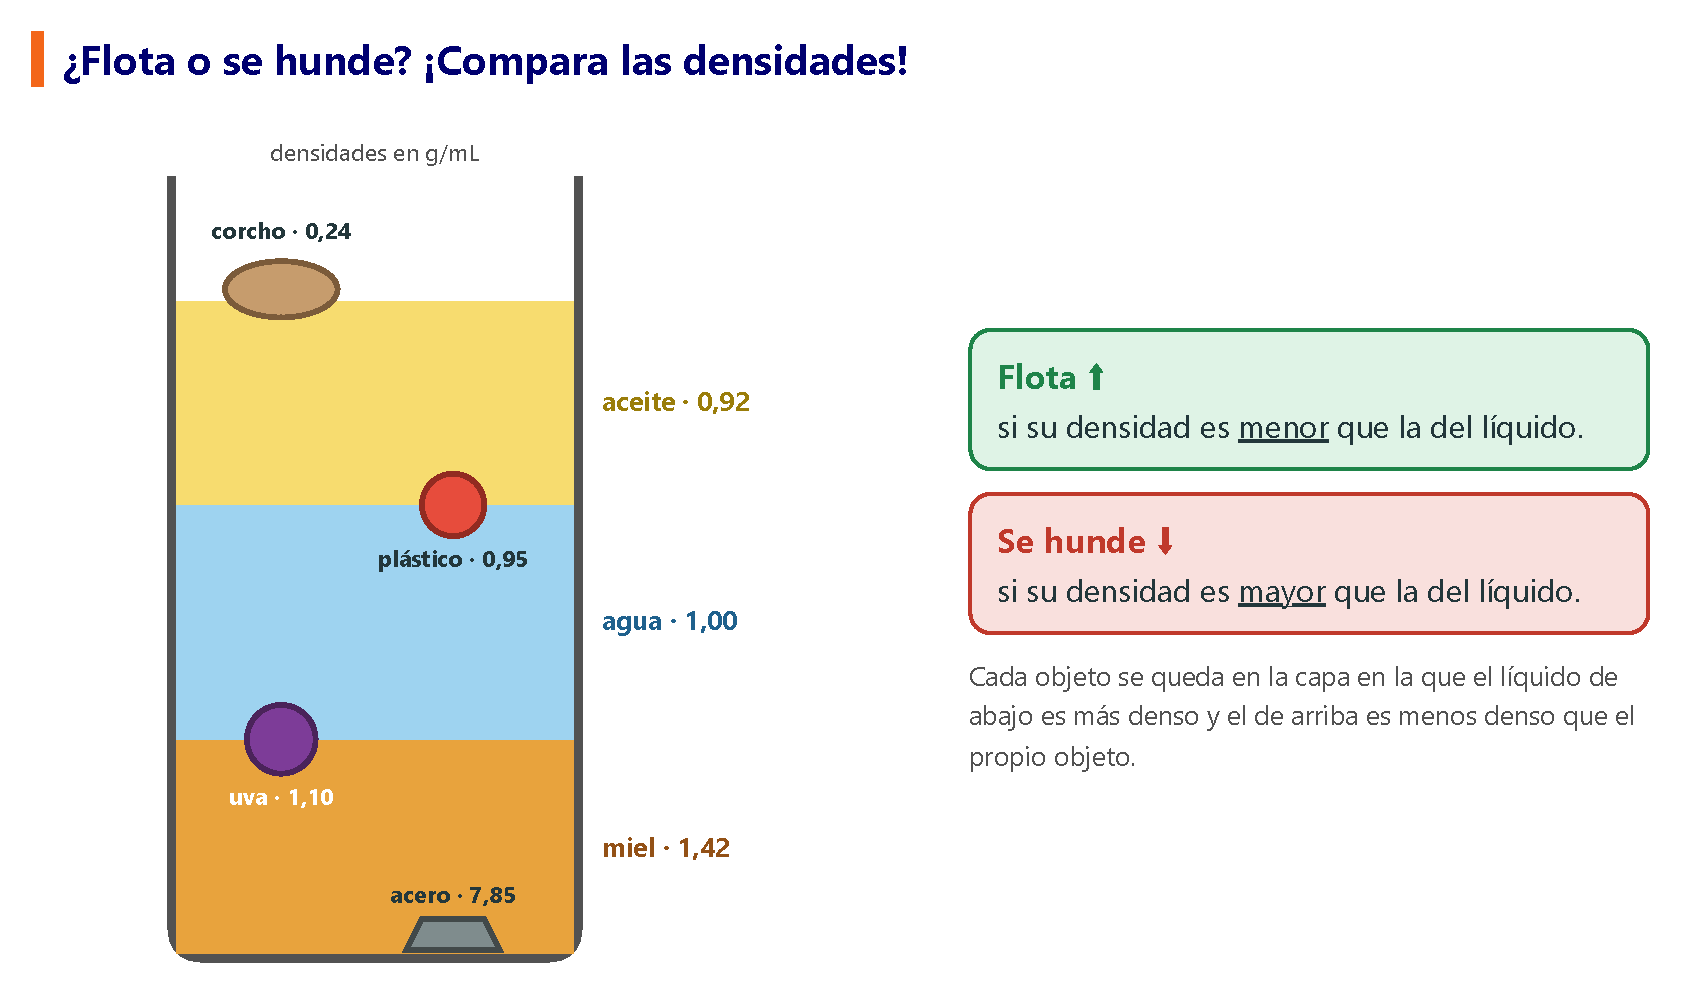
\includegraphics[width=0.95\textwidth]{FigurasSVG/Unit_1_Matter_Measurement/pdf/density_column_es.pdf}
    \caption{Una columna de densidades: cada objeto flota o se hunde según su densidad.}
    \label{fig:u1_density_column}
\end{figure}

\begin{impt}
    En el agua (\(d = \qty{1.00}{\g\per\mL}\)):
    \begin{itemize}
        \item \(d_{\text{objeto}} < \qty{1.00}{\g\per\mL}\) \(\to\) \textbf{flota}.
        \item \(d_{\text{objeto}} > \qty{1.00}{\g\per\mL}\) \(\to\) \textbf{se hunde}.
    \end{itemize}
\end{impt}

\begin{didyouknow}
    El hielo (\qty{0.92}{\g\per\mL}) es menos denso que el agua líquida, así que los icebergs flotan\ldots{} pero cerca del \textbf{90\,\%} de un iceberg está escondido bajo la superficie. ¡De ahí viene la expresión «la punta del iceberg»!
\end{didyouknow}

\begin{exercise}
    Las densidades del corcho, el aluminio y la glicerina son \qty{0.24}{\g\per\mL}, \qty{2.70}{\g\per\mL} y \qty{1.26}{\g\per\mL}, respectivamente.
    \begin{enumerate}[label=\letraminuscula]
        \item ¿Cuáles flotan en el agua (\(d = \qty{1.00}{\g\per\mL}\))?
        \item El mercurio tiene una densidad de \qty{13.6}{\g\per\mL}. ¿Cuáles de los tres materiales flotarían sobre el mercurio?
    \end{enumerate}
    \begin{solu}
        \begin{enumerate}[label=\alph*)]
            \item El corcho flota en el agua (\(0.24 < 1.00\)). El aluminio y la glicerina se hunden (\(2.70 > 1.00\) y \(1.26 > 1.00\)).
            \item Los tres tienen una densidad menor que la del mercurio, así que \textbf{el corcho, el aluminio y la glicerina flotarían sobre el mercurio}.
        \end{enumerate}
    \end{solu}
\end{exercise}

\begin{exercise}
    Un bloque de madera tiene una masa de \qty{45}{\g} y un volumen de \qty{60}{\cubic\cm}.
    \begin{enumerate}[label=\letraminuscula]
        \item Calcula su densidad.
        \item ¿Flotará o se hundirá en el agua? Justifica tu respuesta.
    \end{enumerate}
    \begin{solu}
        \begin{enumerate}[label=\alph*)]
            \item \(d = \dfrac{m}{V} = \dfrac{\qty{45}{\g}}{\qty{60}{\cubic\cm}} = \qty{0.75}{\g\per\cubic\cm}\).
            \item Como \(\qty{0.75}{\g\per\mL} < \qty{1.00}{\g\per\mL}\) (agua), el bloque \textbf{flota}.
        \end{enumerate}
    \end{solu}
\end{exercise}

\begin{exercise}
    Un barco está hecho de acero, que tiene una densidad de unos \qty{7.85}{\g\per\mL}, mucho mayor que la del agua. Explica, usando la idea de densidad, por qué un bloque macizo de acero se hunde y, en cambio, un barco de acero flota.
    \begin{solu}
        Un barco está casi todo hueco (lleno de aire), así que su volumen total es mucho mayor que el de un bloque macizo de acero de la misma masa. Por eso la \textbf{densidad media de todo el barco} es menor que la del agua y flota, aunque el acero por sí solo sea más denso que el agua.
    \end{solu}
\end{exercise}


%----------------------------------------------------------------------------------------

\section{Los instrumentos de medida}

\subsection{Medida de la masa}

\begin{figure}[H]
    \centering
    % [FIGURA ORIGINAL] \includegraphics[width=\textwidth]{Unit_1/balances}
    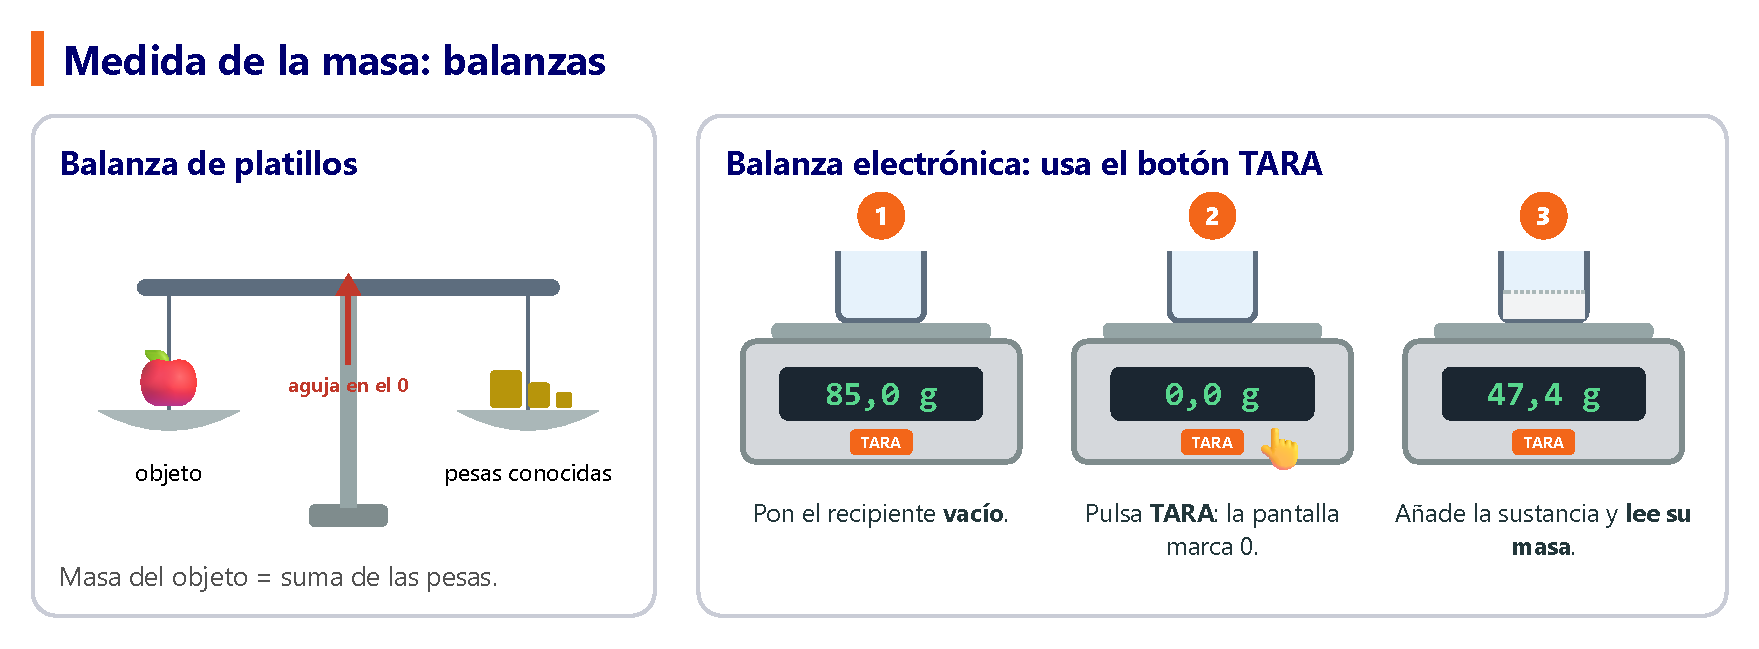
\includegraphics[width=\textwidth]{FigurasSVG/Unit_1_Matter_Measurement/pdf/balances_es.pdf}
    \caption{Una balanza de platillos y una balanza electrónica con su botón TARA.}
    \label{fig:u1_balances}
\end{figure}

\begin{itemize}
    \item \negsubro{Balanza de platillos}: se pone el objeto en un platillo y se añaden pesas conocidas en el otro hasta que la aguja marca 0. Masa del objeto = suma de las pesas.
    \item \negsubro{Balanza electrónica}: se pone el recipiente vacío, se pulsa \textbf{TARA} (la pantalla marca 0) y se añade la sustancia. La pantalla muestra solo la masa de la sustancia.
\end{itemize}

\begin{impt}
    \negsubro{La masa no es el peso}. La \textbf{masa} es la cantidad de materia (\unit{\kg}) y es la misma en todas partes. El \textbf{peso} es la fuerza con la que un planeta atrae a un cuerpo (\unit{\N}): en la Luna pesarías seis veces menos, pero tu masa no cambiaría.
\end{impt}

\begin{exercise}
    Explica por qué pulsamos «tara» antes de añadir una sustancia en una balanza electrónica, en lugar de pesar simplemente el recipiente con la sustancia dentro y restar a mano.
    \begin{solu}
        Al pulsar «tara», la pantalla se pone a cero con el recipiente vacío ya encima de la balanza, así que la masa que se muestra después es directamente la masa de la sustancia sola. Así se ahorra tiempo y se evitan errores de cálculo.
    \end{solu}
\end{exercise}

\begin{exercise}
    Un alumno pone un vaso de precipitados vacío en una balanza electrónica sin pulsar la tara: marca \qty{85.0}{\g}. Después añade algo de sal, y la balanza marca ahora \qty{132.4}{\g}.
    \begin{enumerate}[label=\letraminuscula]
        \item Calcula la masa de la sal.
        \item Explica cómo habría hecho la tara más directa esta medida.
    \end{enumerate}
    \begin{solu}
        \begin{enumerate}[label=\alph*)]
            \item Masa de sal \(= \qty{132.4}{\g} - \qty{85.0}{\g} = \qty{47.4}{\g}\).
            \item Con la tara, la balanza habría marcado \qty{0}{\g} con el vaso vacío, así que la lectura final habría sido directamente \qty{47.4}{\g}.
        \end{enumerate}
    \end{solu}
\end{exercise}


\subsection{Medida del volumen}

\begin{itemize}
    \item \negsubro{Cuerpos regulares} (cubo, prisma, cilindro, esfera\ldots): medimos sus longitudes y usamos una fórmula.
    \item \negsubro{Líquidos y cuerpos irregulares}: usamos una \textbf{probeta}, una \textbf{bureta} o una \textbf{pipeta}.
\end{itemize}

\begin{definition}[Menisco]
    Es la superficie curva de un líquido dentro de un tubo estrecho. El volumen se lee en la \textbf{parte de abajo} del menisco, con los ojos a la misma altura que el líquido.
\end{definition}

\begin{figure}[H]
    \centering
    % [FIGURA ORIGINAL] \includegraphics[width=\textwidth]{Unit_1/meniscus}
    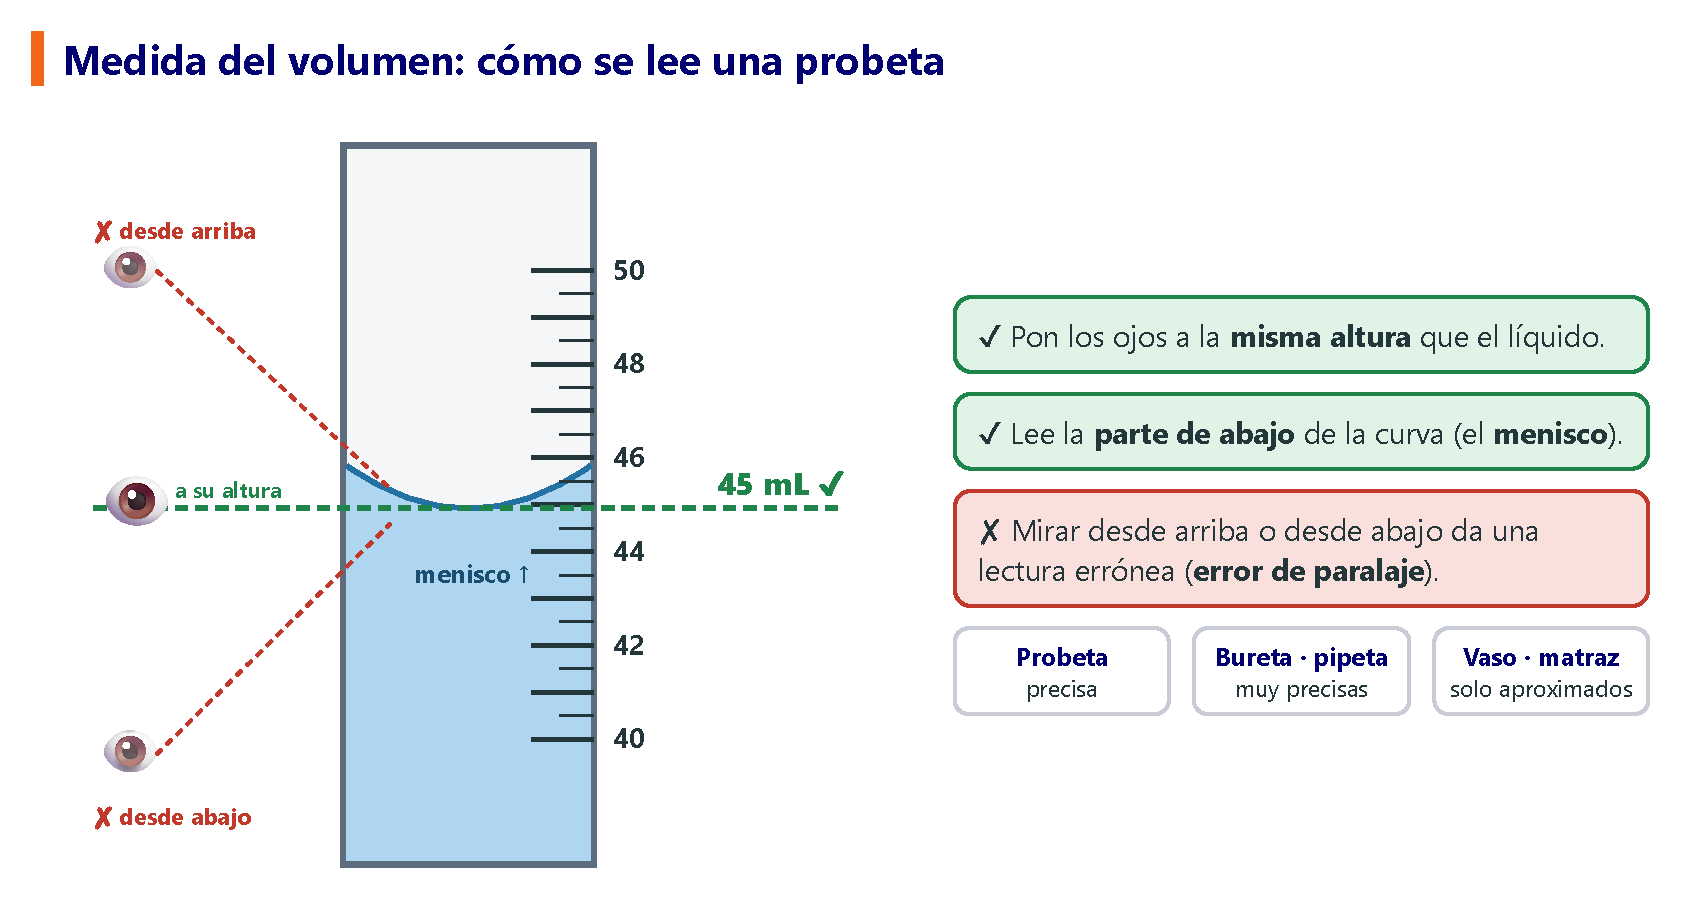
\includegraphics[width=\textwidth]{FigurasSVG/Unit_1_Matter_Measurement/pdf/meniscus_es.pdf}
    \caption{La forma correcta de leer una probeta.}
    \label{fig:u1_meniscus}
\end{figure}

\begin{exercise}
    Una probeta de \qty{25}{\mL} permite medir \qty{0.5}{\mL}, y una de \qty{250}{\mL} permite medir \qty{5}{\mL}. ¿Cuál de las dos da una medida más precisa? ¿Por qué elegirías la pequeña para medir \qty{18}{\mL} de un líquido?
    \begin{solu}
        La probeta de \qty{25}{\mL} es más precisa, porque su división más pequeña (\qty{0.5}{\mL}) es menor. \\
        Para \qty{18}{\mL}, la probeta de \qty{25}{\mL} es la adecuada: el líquido ocupa casi toda la probeta y la lectura es más precisa.
    \end{solu}
\end{exercise}

\begin{exercise}
    Indica qué usarías (la fórmula de un cuerpo regular, una probeta o un matraz Erlenmeyer) para medir el volumen de cada una de estas cosas, y explica por qué:
    \begin{enumerate}[label=\letraminuscula]
        \item Un cubo de madera de \qty{4}{\cm} de arista.
        \item \qty{35}{\mL} de vinagre para una receta.
        \item Una piedra pequeña de forma irregular.
        \item Más o menos cuánta agua queda en una botella.
    \end{enumerate}
    \begin{solu}
        \begin{enumerate}[label=\alph*)]
            \item Es un cuerpo regular: medimos la arista con una regla y usamos \(V = \text{arista}^3\).
            \item Una probeta, porque da una lectura precisa del volumen de un líquido.
            \item Una probeta, midiendo cuánto sube el nivel del agua, ya que la piedra es irregular.
            \item Un matraz Erlenmeyer o un vaso de precipitados, porque solo hace falta un volumen aproximado.
        \end{enumerate}
    \end{solu}
\end{exercise}

\begin{exercise}
    Al leer el volumen de agua en una probeta, ¿por qué tenemos que poner los ojos a la misma altura que la superficie del líquido, y por qué leemos la \textbf{parte de abajo} del menisco y no la de arriba?
    \begin{solu}
        Si miramos desde arriba o desde abajo, la lectura sale demasiado alta o demasiado baja (\textbf{error de paralaje}). Mirando a la altura de los ojos evitamos este error. \\
        Leemos la parte de abajo del menisco porque el agua se pega a las paredes de vidrio y sube un poco por los bordes; la parte de abajo de la curva es el punto que corresponde de verdad al volumen de líquido.
    \end{solu}
\end{exercise}

%----------------------------------------------------------------------------------------

\section{Medidas indirectas}

\begin{definition}[Medida indirecta]
    Es una medida que \textbf{calculamos} a partir de otras magnitudes que hemos medido directamente.
\end{definition}

La masa y la longitud se pueden leer directamente en un instrumento, pero la superficie, la densidad o los grosores muy pequeños normalmente hay que \textbf{calcularlos}.

\subsection{Medida de la densidad}

\begin{itemize}
    \item \negsubro{Líquido}: se tara una probeta en la balanza, se echa el líquido, se leen su volumen \(V\) y su masa \(m\), y se calcula \(d = m/V\).
    \item \negsubro{Sólido que no se disuelve en agua}: se pesa y se mide su volumen por \textbf{desplazamiento de agua}, como muestra la figura.
\end{itemize}

\begin{figure}[H]
    \centering
    % [FIGURA ORIGINAL] \includegraphics[width=\textwidth]{Unit_1/density_lab}
    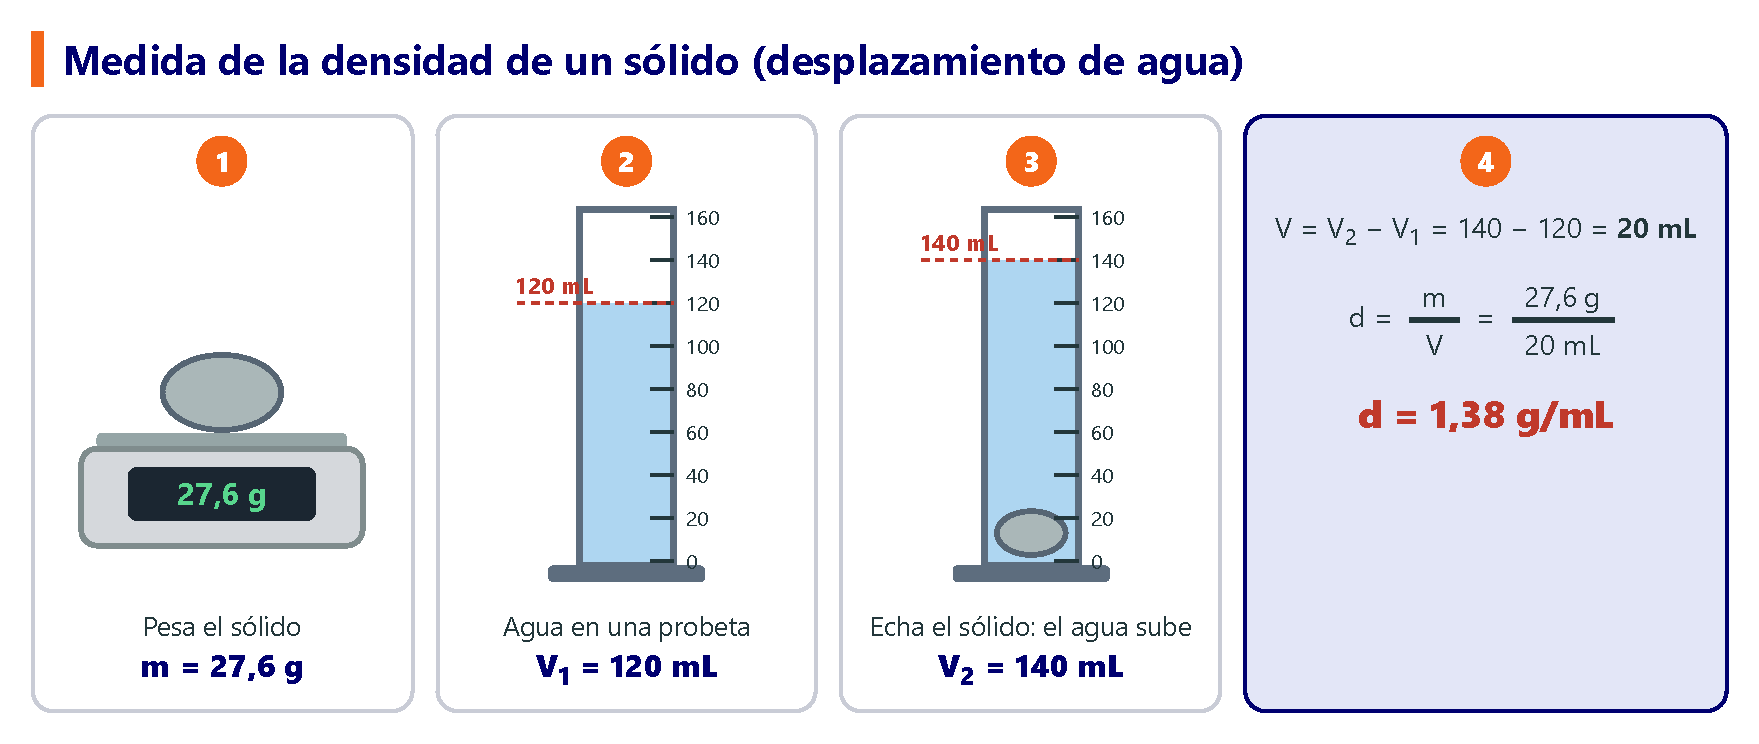
\includegraphics[width=\textwidth]{FigurasSVG/Unit_1_Matter_Measurement/pdf/density_lab_es.pdf}
    \caption{Medida de la densidad de un sólido: el volumen del sólido es lo que sube el nivel del agua.}
    \label{fig:u1_density_lab}
\end{figure}

\begin{didyouknow}
    Según la leyenda, Arquímedes descubrió este método en el baño: al meterse, el nivel del agua subió. Se dio cuenta de que podía usarlo para medir el volumen de la corona del rey y comprobar si era de oro puro. Se emocionó tanto que salió corriendo a la calle gritando «¡Eureka!» («¡Lo he encontrado!»).
\end{didyouknow}

\begin{exercise}
    Un bloque de plastilina tiene una masa de \qty{27.6}{\g}. Al meterlo en una probeta con \qty{120}{\mL} de agua, el nivel sube hasta \qty{140}{\mL}.
    \begin{enumerate}[label=\letraminuscula]
        \item Calcula la densidad de la plastilina.
        \item Si un segundo bloque de la misma plastilina tuviera la mitad de volumen, ¿cuáles serían su masa y su densidad?
    \end{enumerate}
    \begin{solu}
        \begin{enumerate}[label=\alph*)]
            \item \(V = \qty{140}{\mL} - \qty{120}{\mL} = \qty{20}{\mL}\); \(d = \dfrac{\qty{27.6}{\g}}{\qty{20}{\mL}} = \qty{1.38}{\g\per\mL}\).
            \item La mitad de volumen (\qty{10}{\mL}) significa la mitad de masa (\qty{13.8}{\g}). La \textbf{densidad no cambia} (\qty{1.38}{\g\per\mL}), porque es una propiedad característica.
        \end{enumerate}
    \end{solu}
\end{exercise}

\begin{exercise}
    Para medir la densidad del azúcar: masa de la probeta vacía = \qty{130}{\g}; masa de la probeta con el azúcar = \qty{198.5}{\g}; al echar el azúcar en una probeta con \qty{100}{\mL} de un líquido en el que no se disuelve, el nivel sube hasta \qty{130}{\mL}. ¿Cuál es la densidad del azúcar?
    \begin{solu}
        Masa de azúcar \(= \qty{198.5}{\g} - \qty{130}{\g} = \qty{68.5}{\g}\). \\
        Volumen de azúcar \(= \qty{130}{\mL} - \qty{100}{\mL} = \qty{30}{\mL}\). \\
        Densidad: \(d = \dfrac{\qty{68.5}{\g}}{\qty{30}{\mL}} \approx \qty{2.28}{\g\per\mL}\).
    \end{solu}
\end{exercise}

\begin{exercise}
    Las densidades de la leche, el agua y el aceite son \qty{1.04}{\g\per\mL}, \qty{1.00}{\g\per\mL} y \qty{0.92}{\g\per\mL}, respectivamente. Calcula la masa de \qty{1}{\litre} de cada uno.
    \begin{solu}
        Usando \(m = d \cdot V\) con \(V = \qty{1000}{\mL}\): \\
        Leche: \(m = \qty{1.04}{\g\per\mL} \cdot \qty{1000}{\mL} = \qty{1040}{\g}\). \\
        Agua: \(m = \qty{1000}{\g}\). \\
        Aceite: \(m = \qty{920}{\g}\).
    \end{solu}
\end{exercise}

%----------------------------------------------------------------------------------------

\section{El material de laboratorio y las normas de seguridad}

El laboratorio es el lugar donde hacemos experimentos. Es muy divertido\ldots{} pero solo si conocemos el material y cumplimos las normas de seguridad.

\subsection{Material de laboratorio habitual}

\begin{figure}[H]
    \centering
    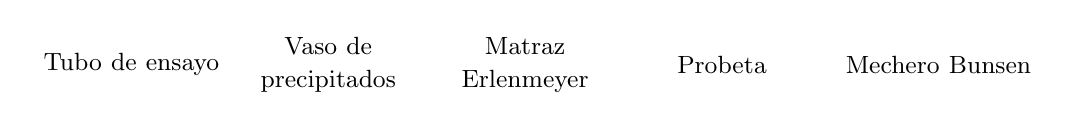
\begin{tikzpicture}[scale=0.5]
        \begin{scope}
            \tkzTestTube[glassType=tube,liquidLevel1=40]
            \node[align=center, text width=2.4cm] at (0,-1) {\small Tubo de ensayo};
        \end{scope}
        \begin{scope}[xshift=5cm]
            \tkzTestTube[glassType=beaker,liquidLevel1=40]
            \node[align=center, text width=2.4cm] at (0,-1) {\small Vaso de precipitados};
        \end{scope}
        \begin{scope}[xshift=10cm]
            \tkzTestTube[glassType=erlenmeyer,liquidLevel1=30]
            \node[align=center, text width=2.4cm] at (0,-1) {\small Matraz Erlenmeyer};
        \end{scope}
        \begin{scope}[xshift=15cm]
            \tkzGraduatedCylinder[liquidLevel1=60]
            \node[align=center, text width=2.4cm] at (0,-1) {\small Probeta};
        \end{scope}
        \begin{scope}[xshift=20.5cm]
            \tkzBunsenBurner
            \node[align=center, text width=2.4cm] at (0,-1) {\small Mechero Bunsen};
        \end{scope}
    \end{tikzpicture}
    \caption{Material de vidrio habitual en el laboratorio y un mechero Bunsen, dibujados con el paquete \texttt{tikz-chemlab}.}
    \label{fig:glassware}
\end{figure}

\begin{table}[H]
    \centering
    \small
    \renewcommand{\arraystretch}{1.35}
    \begin{tabular}{p{3.3cm}p{9.5cm}}
        \toprule
        \textbf{Material} & \textbf{Para qué lo usamos} \\
        \midrule
        Tubo de ensayo & contener, calentar o mezclar cantidades \textbf{pequeñas} de sustancias \\
        Vaso de precipitados & mezclar o calentar líquidos; medir volúmenes \textbf{aproximados} \\
        Matraz Erlenmeyer & mezclar o calentar líquidos sin que se derramen (cuello estrecho) \\
        Probeta & medir el volumen de un líquido con \textbf{precisión} \\
        Mechero Bunsen & fuente de calor (llama de gas) \\
        \bottomrule
    \end{tabular}
    \caption{Material básico de laboratorio y sus usos.}
    \label{tab:u1_lab_material}
\end{table}

\subsection{La seguridad en el laboratorio}

\begin{figure}[H]
    \centering
    % [FIGURA ORIGINAL] \includegraphics[width=\textwidth]{Unit_1/lab_safety}
    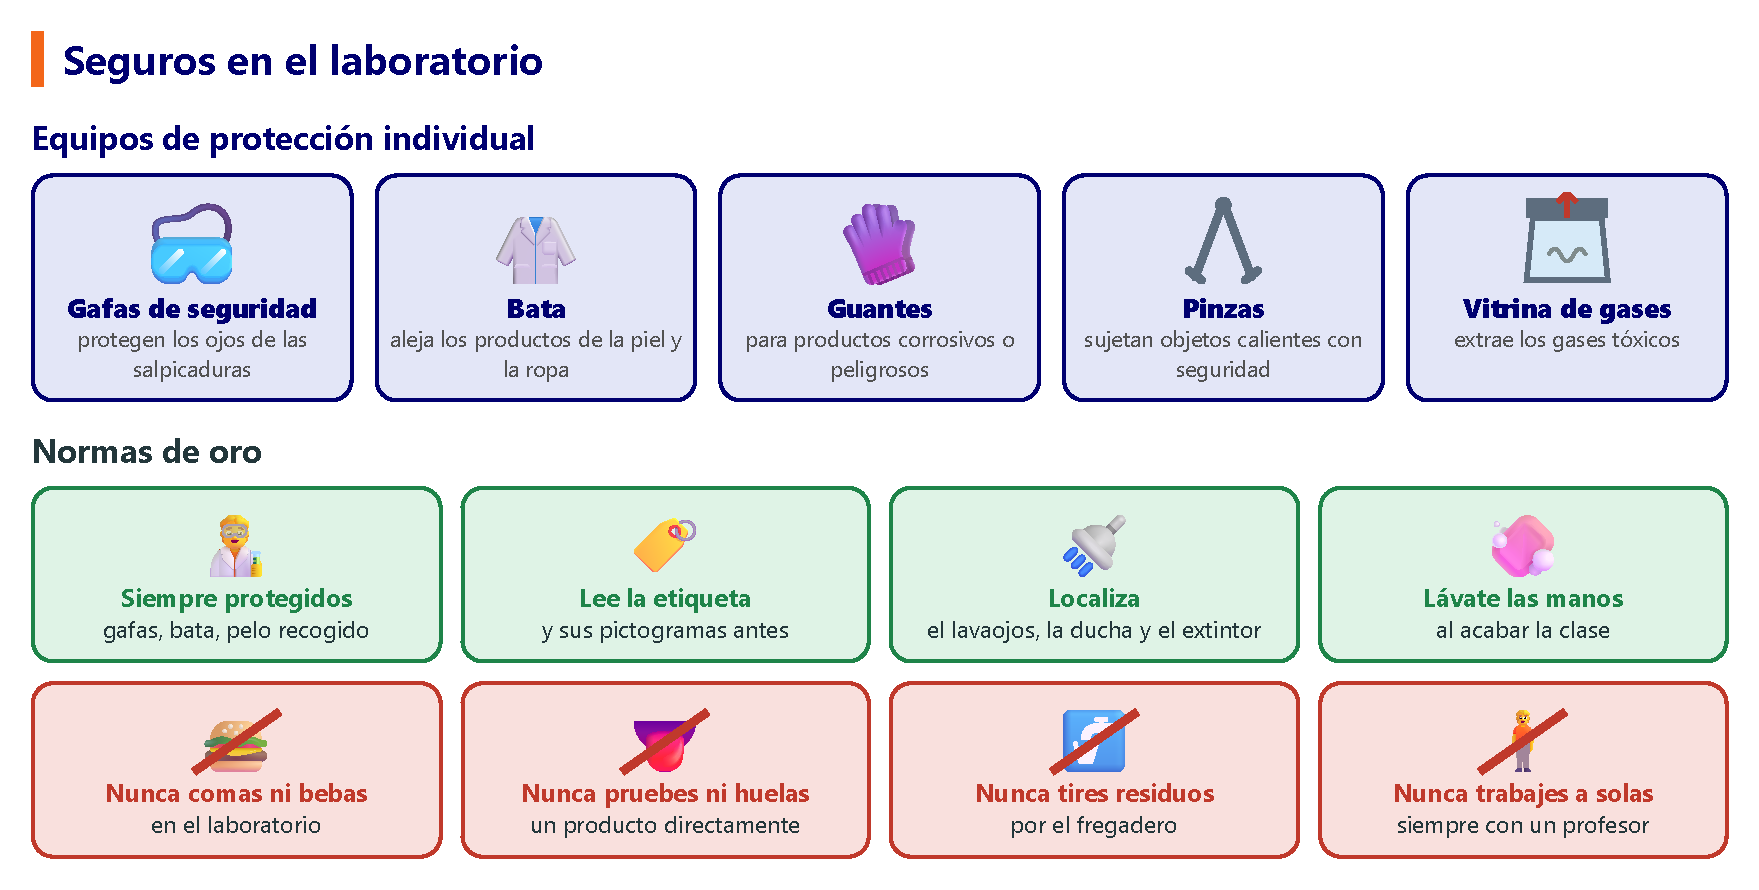
\includegraphics[width=\textwidth]{FigurasSVG/Unit_1_Matter_Measurement/pdf/lab_safety_es.pdf}
    \caption{Equipos de protección individual y normas de oro del laboratorio.}
    \label{fig:u1_lab_safety}
\end{figure}

Dos normas más que se olvidan con facilidad:
\begin{enumerate}[label=\numberballmDarkTeal]
    \item Apunta un tubo de ensayo que se está calentando \textbf{lejos} de ti y de las demás personas.
    \item Mantén ordenada tu mesa y usa solo el material y las cantidades que te indique tu profesor o profesora.
\end{enumerate}


\subsection{Pictogramas de peligrosidad (SGA)}

\begin{definition}[Pictograma de peligrosidad]
    Es un símbolo normalizado, negro sobre fondo blanco dentro de un rombo rojo, que aparece en la etiqueta de un producto químico para avisarnos, de un vistazo, del tipo de peligro que presenta. El conjunto actual lo fija el \negsubro{Sistema Globalmente Armonizado (SGA)}, que se usa en todo el mundo.
\end{definition}

\begin{figure}[H]
    \centering
    \begin{tabular}{@{}p{5.0cm}p{5.0cm}p{5.0cm}@{}}
        \begin{minipage}{5.0cm}
            \centering
            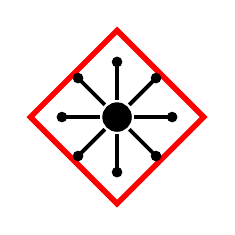
\begin{tikzpicture}
                \draw[draw=red, line width=2pt, fill=white] (0,-1.1) -- (1.1,0) -- (0,1.1) -- (-1.1,0) -- cycle;
                \filldraw[black] (0,0) circle (0.18);
                \foreach \a in {0,45,90,135,180,225,270,315}{
                    \draw[line width=1.4pt] (\a:0.22) -- (\a:0.65);
                    \filldraw[black] (\a:0.7) circle (0.06);
                }
            \end{tikzpicture}\\[2pt]
            \textbf{Explosivo}\\[2pt]
            {\small Puede explotar con el calor, un golpe o el rozamiento. Ejemplo: fuegos artificiales.}
        \end{minipage}
        &
        \begin{minipage}{5.0cm}
            \centering
            
\begin{tikzpicture}
                \draw[draw=red, line width=2pt, fill=white] (0,-1.1) -- (1.1,0) -- (0,1.1) -- (-1.1,0) -- cycle;
                \fill[black] plot [smooth cycle] coordinates {(0,-0.75) (0.32,-0.35) (0.22,0.05) (0.42,0.35) (0.12,0.75) (-0.15,0.35) (-0.32,0.0) (-0.18,-0.35)};
                \fill[white] plot [smooth cycle] coordinates {(0,-0.4) (0.14,-0.1) (0.05,0.15) (0.14,0.35) (0,0.55) (-0.1,0.3) (-0.14,0.0) (-0.05,-0.2)};
            \end{tikzpicture}\\[2pt]
            \textbf{Inflamable}\\[2pt]
            {\small Arde con facilidad. Ejemplo: alcohol, gasolina.}
        \end{minipage}
        &
        \begin{minipage}{5.0cm}
            \centering
            
\begin{tikzpicture}
                \draw[draw=red, line width=2pt, fill=white] (0,-1.1) -- (1.1,0) -- (0,1.1) -- (-1.1,0) -- cycle;
                \draw[line width=1.6pt] (0,-0.85) circle (0.2);
                \begin{scope}[yshift=0.15cm]
                    \fill[black] plot [smooth cycle] coordinates {(0,-0.75) (0.32,-0.35) (0.22,0.05) (0.42,0.35) (0.12,0.75) (-0.15,0.35) (-0.32,0.0) (-0.18,-0.35)};
                \end{scope}
            \end{tikzpicture}\\[2pt]
            \textbf{Comburente}\\[2pt]
            {\small Aviva el fuego y hace que arda con más fuerza. Ejemplo: lejía, botellas de oxígeno.}
        \end{minipage}
        \\[9mm]
        \begin{minipage}{5.0cm}
            \centering
            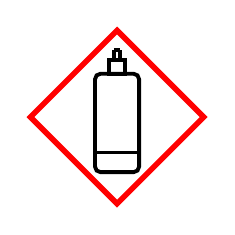
\begin{tikzpicture}
                \draw[draw=red, line width=2pt, fill=white] (0,-1.1) -- (1.1,0) -- (0,1.1) -- (-1.1,0) -- cycle;
                \draw[line width=1.4pt, rounded corners=2pt] (-0.28,-0.7) rectangle (0.28,0.55);
                \draw[line width=1.4pt] (-0.1,0.55) rectangle (0.1,0.72);
                \draw[line width=1.4pt] (-0.04,0.72) -- (-0.04,0.85);
                \draw[line width=1.4pt] (0.04,0.72) -- (0.04,0.85);
                \draw[line width=1.4pt] (-0.04,0.85) -- (0.04,0.85);
                \draw[line width=1pt] (-0.28,-0.45) -- (0.28,-0.45);
            \end{tikzpicture}\\[2pt]
            \textbf{Gas a presión}\\[2pt]
            {\small Gas guardado a presión; puede explotar si se calienta. Ejemplo: bombonas de gas.}
        \end{minipage}
        &
        \begin{minipage}{5.0cm}
            \centering
            
\begin{tikzpicture}
                \draw[draw=red, line width=2pt, fill=white] (0,-1.1) -- (1.1,0) -- (0,1.1) -- (-1.1,0) -- cycle;
                \begin{scope}[rotate=20, shift={(-0.35,0.55)}]
                    \draw[line width=1.2pt] (-0.1,-0.35) -- (-0.1,0.35) arc (180:0:0.1) -- (0.1,-0.35) -- cycle;
                \end{scope}
                \begin{scope}[rotate=-20, shift={(0.35,0.55)}]
                    \draw[line width=1.2pt] (-0.1,-0.35) -- (-0.1,0.35) arc (180:0:0.1) -- (0.1,-0.35) -- cycle;
                \end{scope}
                \draw[line width=1pt] (-0.15,0.15) -- (-0.05,-0.05);
                \draw[line width=1pt] (0.15,0.15) -- (0.05,-0.05);
                \fill[black] (-0.45,-0.15) -- (0.45,-0.15) -- (0.4,-0.3) -- (0.3,-0.18) -- (0.2,-0.32) -- (0.1,-0.16) -- (0,-0.3) -- (-0.1,-0.16) -- (-0.2,-0.3) -- (-0.3,-0.16) -- (-0.4,-0.28) -- cycle;
                \draw[line width=1.2pt] (-0.4,-0.55) .. controls (-0.2,-0.75) and (0.2,-0.75) .. (0.4,-0.55) -- (0.4,-0.85) -- (-0.4,-0.85) -- cycle;
                \draw[line width=0.8pt] (-0.05,-0.6) -- (-0.02,-0.75);
                \draw[line width=0.8pt] (0.1,-0.62) -- (0.13,-0.78);
            \end{tikzpicture}\\[2pt]
            \textbf{Corrosivo}\\[2pt]
            {\small Quema la piel y los ojos, y puede destruir los metales. Ejemplo: lejía, desatascadores.}
        \end{minipage}
        &
        \begin{minipage}{5.0cm}
            \centering
            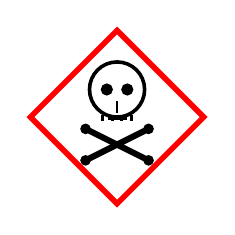
\begin{tikzpicture}
                \draw[draw=red, line width=2pt, fill=white] (0,-1.1) -- (1.1,0) -- (0,1.1) -- (-1.1,0) -- cycle;
                \draw[line width=1.3pt] (0,0.35) circle (0.35);
                \filldraw[black] (-0.13,0.35) circle (0.07);
                \filldraw[black] (0.13,0.35) circle (0.07);
                \draw[line width=1pt] (0,0.2) -- (0,0.05);
                \draw[line width=1pt] (-0.12,-0.02) -- (0.12,-0.02);
                \draw[line width=1pt] (-0.18,-0.05) -- (-0.18,0.02);
                \draw[line width=1pt] (-0.06,-0.05) -- (-0.06,0.02);
                \draw[line width=1pt] (0.06,-0.05) -- (0.06,0.02);
                \draw[line width=1pt] (0.18,-0.05) -- (0.18,0.02);
                \draw[line width=2.2pt] (-0.4,-0.55) -- (0.4,-0.15);
                \draw[line width=2.2pt] (-0.4,-0.15) -- (0.4,-0.55);
                \filldraw[black] (-0.4,-0.55) circle (0.06);
                \filldraw[black] (0.4,-0.15) circle (0.06);
                \filldraw[black] (-0.4,-0.15) circle (0.06);
                \filldraw[black] (0.4,-0.55) circle (0.06);
            \end{tikzpicture}\\[2pt]
            \textbf{Tóxico}\\[2pt]
            {\small Puede matar o causar daños graves, incluso en cantidades pequeñas. Ejemplo: algunos pesticidas.}
        \end{minipage}
        \\[9mm]
        \begin{minipage}{5.0cm}
            \centering
            
\begin{tikzpicture}
                \draw[draw=red, line width=2pt, fill=white] (0,-1.1) -- (1.1,0) -- (0,1.1) -- (-1.1,0) -- cycle;
                \draw[line width=5pt, line cap=round] (0,-0.05) -- (0,0.65);
                \filldraw[black] (0,-0.45) circle (0.1);
            \end{tikzpicture}\\[2pt]
            \textbf{Nocivo / Irritante}\\[2pt]
            {\small Irrita la piel o los ojos, o es nocivo si se traga. Ejemplo: algunos detergentes.}
        \end{minipage}
        &
        \begin{minipage}{5.0cm}
            \centering
            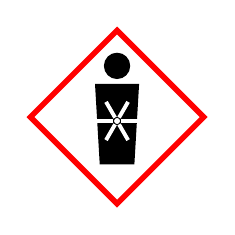
\begin{tikzpicture}
                \draw[draw=red, line width=2pt, fill=white] (0,-1.1) -- (1.1,0) -- (0,1.1) -- (-1.1,0) -- cycle;
                \filldraw[black] (0,0.65) circle (0.16);
                \fill[black] (-0.28,0.42) -- (0.28,0.42) -- (0.22,-0.6) -- (-0.22,-0.6) -- cycle;
                \begin{scope}[shift={(0,-0.05)}]
                    \foreach \a in {0,60,120,180,240,300}{
                        \draw[white, line width=1.4pt] (\a:0.05) -- (\a:0.28);
                    }
                \end{scope}
                \filldraw[white] (0,-0.05) circle (0.03);
            \end{tikzpicture}\\[2pt]
            \textbf{Peligro para la salud}\\[2pt]
            {\small Puede causar daños graves a largo plazo (por ejemplo, en los pulmones). Ejemplo: humo del tabaco, amianto.}
        \end{minipage}
        &
        \begin{minipage}{5.0cm}
            \centering
            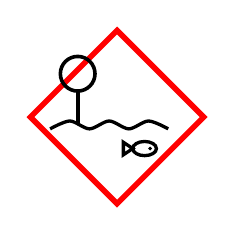
\begin{tikzpicture}
                \draw[draw=red, line width=2pt, fill=white] (0,-1.1) -- (1.1,0) -- (0,1.1) -- (-1.1,0) -- cycle;
                \draw[line width=1.4pt] (-0.5,-0.1) -- (-0.5,0.35);
                \draw[line width=1.3pt] (-0.5,0.55) circle (0.22);
                \draw[line width=1.2pt] plot[smooth] coordinates {(-0.85,-0.15) (-0.6,-0.05) (-0.35,-0.15) (-0.1,-0.05) (0.15,-0.15) (0.4,-0.05) (0.65,-0.15)};
                \draw[line width=1.2pt] (0.35,-0.4) ellipse (0.15 and 0.09);
                \draw[line width=1.2pt] (0.2,-0.4) -- (0.08,-0.32) -- (0.08,-0.48) -- cycle;
                \filldraw[black] (0.42,-0.4) circle (0.015);
            \end{tikzpicture}\\[2pt]
            \textbf{Peligro para el medio ambiente}\\[2pt]
            {\small Venenoso para las plantas, los peces u otros seres vivos. Ejemplo: algunos pesticidas y disolventes.}
        \end{minipage}
    \end{tabular}
    \caption{Los nueve pictogramas de peligrosidad del SGA: un símbolo negro sobre fondo blanco, dentro de un rombo rojo.}
\end{figure}

\begin{impt}
    Un mismo producto puede llevar más de un pictograma a la vez (por ejemplo, un desatascador puede ser corrosivo y tóxico). Lee siempre \textbf{todos} los pictogramas de una etiqueta antes de usar un producto.
\end{impt}

\begin{exercise}
    Una botella de ácido clorhídrico concentrado lleva el pictograma de \negsubro{corrosivo}, y una botella de etanol lleva el de \negsubro{inflamable}. Explica con tus palabras de qué peligro avisa cada pictograma y di una medida de seguridad que debes tomar con cada producto.
    \begin{solu}
        El pictograma de \textbf{corrosivo} avisa de que el ácido puede quemar la piel y los ojos y dañar los materiales al entrar en contacto con ellos, así que debemos usar guantes y gafas y evitar cualquier contacto con la piel. \\
        El pictograma de \textbf{inflamable} avisa de que el etanol arde con facilidad, así que debemos mantenerlo lejos de llamas y de fuentes de calor, como un mechero Bunsen encendido.
    \end{solu}
\end{exercise}

\begin{exercise}
    Un alumno va a calentar con un mechero Bunsen un tubo de ensayo que contiene un líquido y, cuando se enfríe, va a medir su volumen.
    \begin{enumerate}[label=\letraminuscula]
        \item Enumera el material y los equipos de seguridad que debe usar durante toda la actividad.
        \item Explica por qué el tubo de ensayo tiene que apuntar lejos de las personas mientras se calienta.
    \end{enumerate}
    \begin{solu}
        \begin{enumerate}[label=\alph*)]
            \item Gafas de seguridad, bata, pinzas para sujetar el tubo de ensayo caliente, un mechero Bunsen, un tubo de ensayo y una probeta para medir el volumen del líquido cuando se haya enfriado.
            \item Los líquidos calientes pueden salpicar o el contenido del tubo puede salir disparado de golpe; si el tubo apunta lejos de las personas, nadie se quema si eso ocurre.
        \end{enumerate}
    \end{solu}
\end{exercise}

\begin{exercise}
    En una sesión de laboratorio, una alumna se come un bocadillo mientras espera a que termine un experimento, no se recoge el pelo largo antes de encender el mechero Bunsen y, al final de la clase, tira por el fregadero el producto químico que le ha sobrado.
    \begin{enumerate}[label=\letraminuscula]
        \item Identifica las tres normas de seguridad que no se han cumplido.
        \item Para cada una, explica brevemente qué tendría que haber hecho.
    \end{enumerate}
    \begin{solu}
        \begin{enumerate}[label=\alph*)]
            \item Comer en el laboratorio; trabajar con una llama con el pelo largo suelto; tirar residuos químicos por el fregadero.
            \item Nunca se puede entrar comida ni bebida en el laboratorio; el pelo largo hay que recogerlo siempre antes de usar una llama, para que no se prenda; los residuos químicos se echan en el recipiente de residuos correcto y etiquetado, nunca por el fregadero.
        \end{enumerate}
    \end{solu}
\end{exercise}

%----------------------------------------------------------------------------------------

\section*{Resumen}

\begin{itemize}
    \item \textbf{Materia}: todo lo que tiene masa y ocupa un espacio. Forma \textbf{cuerpos} (límites definidos) o \textbf{sistemas materiales} (sin límites definidos).
    \item \textbf{Propiedades}: cuantitativas/cualitativas, extensivas/intensivas, generales/características (densidad, temperaturas de fusión y de ebullición, solubilidad, conductividad, dureza).
    \item \textbf{Densidad y flotación}: una sustancia flota en un líquido si su densidad es menor que la del líquido, y se hunde si es mayor.
    \item \textbf{Despejar una magnitud}: hacemos la misma operación en los dos lados de la ecuación: \(d = m/V\), \(m = d \cdot V\), \(V = m/d\).
    \item \textbf{Magnitud, unidad, medida}: una magnitud se mide comparándola con una unidad; el SI fija las unidades, los múltiplos y los submúltiplos de cada magnitud.
    \item \textbf{Magnitudes fundamentales y derivadas}: el SI tiene siete magnitudes fundamentales (longitud, masa, tiempo, temperatura, cantidad de sustancia, intensidad de corriente e intensidad luminosa); todas las demás (superficie, volumen, densidad, velocidad, presión, energía\ldots) se derivan de ellas.
    \item \textbf{Múltiplos y submúltiplos}: prefijos (giga, mega, kilo, hecto, deca, deci, centi, mili, micro, nano) que valen una potencia de 10 y permiten escribir las medidas con números sencillos.
    \item \textbf{Factor de conversión}: fracción de dos cantidades iguales en unidades distintas, que vale 1 y sirve para cambiar la unidad de una cantidad sin cambiar su valor. El 1 va siempre con la unidad mayor, y usamos potencias de 10.
    \item \textbf{Longitud, masa y capacidad}: escalones de \(10\); \textbf{superficie}: el factor de la longitud se eleva al cuadrado (escalones de \(10^{2}\)); \textbf{volumen}: el factor de la longitud se eleva al cubo (escalones de \(10^{3}\)).
    \item \textbf{Volumen--capacidad}: \(\qty{1}{\cubic\metre} = \qty{1}{\kilo\litre}\); \(\qty{1}{\cubic\dm} = \qty{1}{\litre}\); \(\qty{1}{\cubic\cm} = \qty{1}{\mL}\).
    \item \textbf{Tiempo}: \(\qty{1}{\minute} = \qty{60}{\s}\), \(\qty{1}{\hour} = \qty{3600}{\s}\), \(\qty{1}{\day} = \qty{24}{\hour}\), 1 semana = 7 días, 1 año = 365 días. La \textbf{velocidad} y la \textbf{densidad} necesitan dos factores de conversión.
    \item \textbf{Notación científica}: \(a \cdot 10^{n}\), con una sola cifra distinta de cero delante de la coma. Números grandes \(\to\) la coma salta a la izquierda, exponente positivo; números pequeños \(\to\) la coma salta a la derecha, exponente negativo.
    \item \textbf{Presión y energía}: \(\qty{1}{\atmospher} = \qty{760}{\mmhg} = \qty{101325}{\Pa}\); \(\qty{1}{\calorie} = \qty{4.18}{\J}\).
    \item \textbf{Instrumentos}: balanzas para la masa; probetas, buretas y pipetas para el volumen (se lee en la parte de abajo del menisco).
    \item \textbf{Medida indirecta}: una magnitud que se calcula a partir de otras medidas directamente (superficie, densidad, grosores pequeños\ldots).
    \item \textbf{Material de laboratorio}: tubos de ensayo, vasos de precipitados, matraces Erlenmeyer, probetas y mecheros Bunsen, que se usan junto con gafas de seguridad, bata y vitrina de gases.
    \item \textbf{Normas de seguridad}: usa siempre el equipo de protección, no comas ni trabajes nunca a solas, conoce dónde están el lavaojos y el extintor, y desecha los residuos correctamente.
    \item \textbf{Pictogramas de peligrosidad (SGA)}: nueve símbolos normalizados, negros sobre fondo blanco dentro de un rombo rojo, que avisan de los peligros de un producto químico (explosivo, inflamable, comburente, gas a presión, corrosivo, tóxico, nocivo/irritante, peligro para la salud, peligro para el medio ambiente).
\end{itemize}

\section{Vocabulario}

\begin{vocabulary}[Materia (\textit{matter})]
    Todo lo que ocupa un espacio y tiene masa.
\end{vocabulary}

\begin{vocabulary}[Cuerpo (\textit{body})]
    Materia con límites definidos.
\end{vocabulary}

\begin{vocabulary}[Sistema material (\textit{material system})]
    Materia sin límites definidos.
\end{vocabulary}

\begin{vocabulary}[Propiedad (\textit{property})]
    Aspecto de la materia que se puede evaluar.
\end{vocabulary}

\begin{vocabulary}[Magnitud (\textit{quantity})]
    Propiedad de la materia que se puede medir.
\end{vocabulary}

\begin{vocabulary}[Magnitud fundamental (\textit{fundamental quantity})]
    Magnitud que se define por sí misma, sin usar otras magnitudes (longitud, masa, tiempo\ldots).
\end{vocabulary}

\begin{vocabulary}[Magnitud derivada (\textit{derived quantity})]
    Magnitud que se obtiene combinando magnitudes fundamentales (superficie, volumen, velocidad\ldots).
\end{vocabulary}

\begin{vocabulary}[Prefijo (\textit{prefix})]
    Palabra o símbolo que se pone delante de una unidad para formar un múltiplo o un submúltiplo de ella (kilo-, centi-\ldots).
\end{vocabulary}

\begin{vocabulary}[Múltiplo / Submúltiplo (\textit{multiple / submultiple})]
    Unidad mayor / menor que la unidad básica en una potencia de 10.
\end{vocabulary}

\begin{vocabulary}[Unidad (\textit{unit})]
    Cantidad conocida de una magnitud que se usa como referencia para medir.
\end{vocabulary}

\begin{vocabulary}[Densidad (\textit{density})]
    Masa por unidad de volumen.
\end{vocabulary}

\begin{vocabulary}[Solubilidad (\textit{solubility})]
    Cantidad máxima de un soluto que se puede disolver en \qty{100}{\g} de disolvente.
\end{vocabulary}

\begin{vocabulary}[Flotación (\textit{floating})]
    Situación en la que una sustancia colocada en un líquido se queda en la superficie porque su densidad es menor que la del líquido.
\end{vocabulary}

\begin{vocabulary}[Menisco (\textit{meniscus})]
    Curva que forma la superficie de un líquido dentro de un tubo estrecho.
\end{vocabulary}

\begin{vocabulary}[Medida indirecta (\textit{indirect measurement})]
    Medida que se obtiene mediante cálculos a partir de otras medidas directas.
\end{vocabulary}

\begin{vocabulary}[Factor de conversión (\textit{conversion factor})]
    Fracción de dos cantidades iguales expresadas en unidades distintas, que se usa para cambiar de unidades.
\end{vocabulary}

\begin{vocabulary}[Notación científica (\textit{scientific notation})]
    Forma de escribir un número como un coeficiente (del 1 al 9,99\ldots) multiplicado por una potencia de 10.
\end{vocabulary}

\begin{vocabulary}[Exponente (\textit{exponent})]
    Número pequeño que se escribe arriba a la derecha de una potencia; nos dice cuántas veces multiplicamos (o dividimos) por 10.
\end{vocabulary}

\begin{vocabulary}[Despejar una magnitud (\textit{to isolate a quantity})]
    Dejar una magnitud sola en un lado de una ecuación, haciendo la misma operación en los dos lados.
\end{vocabulary}

\begin{vocabulary}[Pictograma de peligrosidad (\textit{hazard pictogram})]
    Símbolo normalizado de la etiqueta de un producto químico que avisa del tipo de peligro que presenta.
\end{vocabulary}

\begin{vocabulary}[Corrosivo (\textit{corrosive})]
    Que puede quemar la piel y los ojos y destruir los materiales al entrar en contacto con ellos.
\end{vocabulary}

\begin{vocabulary}[Inflamable (\textit{flammable})]
    Que arde con facilidad.
\end{vocabulary}

\begin{vocabulary}[Vitrina de gases (\textit{fume hood})]
    Armario ventilado que extrae del laboratorio los gases o vapores peligrosos.
\end{vocabulary}

\begin{vocabulary}[Gafas de seguridad (\textit{safety goggles})]
    Gafas que protegen los ojos de salpicaduras, polvo y vapores.
\end{vocabulary}

\begin{vocabulary}[Mechero Bunsen (\textit{Bunsen burner})]
    Quemador de gas que se usa como fuente de calor en el laboratorio.
\end{vocabulary}

